\documentclass[10pt, oneside]{article}

\input ./combined_macros.sty

\newcommand{\BV}{\mathrm{BV}}
\newcommand{\Cl}{\mathrm{Cl}}
\newcommand{\Dens}{\mathrm{Dens}}
\newcommand{\gauge}{\mathrm{gauge}}
\newcommand{\matter}{\mathrm{matter}}
\renewcommand{\Re}{\mathrm{Re}}
\newcommand{\U}{\mathrm{U}}

\newcommand{\defterm}[1]{\textbf{\emph{#1}}}

\addbibresource{Twist.bib}

\usepackage{pdflscape}
\usetikzlibrary{shapes.geometric, arrows, positioning}

\tikzstyle{s16} = [rectangle, rounded corners, minimum width=1.8cm, minimum height=1cm,text centered, draw=black,fill=red!30]
\tikzstyle{s16chiral} = [s16, dashed]
\tikzstyle{s8} = [rectangle, rounded corners, minimum width=1.8cm, minimum height=1cm,text centered, draw=black,fill=orange!30]
\tikzstyle{s4} = [rectangle, rounded corners, minimum width=1.8cm, minimum height=1cm,text centered, draw=black,fill=yellow!30]
\tikzstyle{s2chiral} = [rectangle, dashed, rounded corners, minimum width=1.8cm, minimum height=1cm,text centered, draw=black,fill=green!30]
\tikzstyle{dimension} = [circle, text centered, text width=0.7cm, minimum height=0.7cm, draw=black]
\tikzstyle{arrow} = [thick,->,>=stealth]

\title{Twists of supersymmetric gauge theories}
\author{Chris Elliott\and Pavel Safronov \and Brian Williams}

\date{\today}

\begin{document}

\maketitle

\tableofcontents

\section*{Introduction}

\part{Supersymmetric Gauge Theory}

\section{The BV-BRST Formalism}

Throughout the paper we will mostly work with a $\ZZ\times\ZZ/2$-grading. \emph{Degree} will refer to the first (cohomological) grading and \emph{odd} or \emph{even} to the second (fermionic) grading. For an element $x$ we denote by $|x|\in\ZZ/2$ the total degree.

Given a vector bundle $E\rightarrow M$ we denote by $\cE$ the topological vector space of smooth sections of $E$ and $\cE_c$ the topological vector space of smooth compactly supported sections.
We denote by $\cO(\cE)$ (respectively $\cO(\cE_c)$) the completed algebra of functions on $\cE$ (respectively $\cE_c)$. 
For conventions on functions on topological vector spaces we refer to Appendix \ref{appx: top}. 
We denote by $\oloc(\cE)$ the space of local functionals on $\cE$ (see \cite[Definition 4.5.1.1]{Book2}). An element of $\oloc(\cE)$ will be denoted by
\[\int_M f (\phi, \phi', \dots),\]
where $f$ is a density on $M$ depending on infinite jets of sections of $E$. Note, however, that the integral here is a formal symbol. 
The space of local functionals can be viewed as a subspace
\[
\oloc(\cE) \subset \cO(\cE_c)
\]
where we the integral symbol makes sense in earnest on sections which are compactly supported.
We denote by $\oloc^+(\cE)\subset \oloc(\cE)$ the subspace of local functionals which are at least cubic.

Given two vector bundles $E, F$ on $M$ we can also make sense of the space of local functionals from $E$ to $F$.
By definition, this is 
\[
{\rm Fun}_{\rm loc}(\cE, \cF) = \prod_{n \geq 0} {\rm PolyDiff}(\cE^{\times n}, \cF)_{S_n}
\]
where ${\rm PolyDiff}(\cE^{\times n}, \cF)$ denotes the space of polydifferential operators, and we take coinvariants for the obvious symmetric group action.
When $\cF = \cE$, we refer to ${\rm Fun}_{\rm loc}(\cE, \cE)$ as the space of local vector fields on $E$. 
There is a natural Lie bracket on ${\rm Fun}_{\rm loc}(\cE, \cE)$ and a canonical action of this Lie algebra on local functionals. 

\subsection{Classical BV Theories}

\begin{definition}
A \defterm{free BV theory} on a manifold $M$ is the data:
\begin{itemize}
\item a finite rank $\ZZ\times\ZZ/2$-graded vector bundle $E \to M$ equipped with an even differential operator of cohomological degree $+1$
\[
Q_{\mr{BV}} \colon \cE \to \cE [1] 
\]
such that $(1)$: $Q_{\mr{BV}}^2 = 0$ and $(2)$: the pair $(\cE , Q_{\mr{BV}})$ is an elliptic complex;
\item a map of bundles
\[
\omega\colon E \otimes E \to \Dens_M [-1]
\]
that is
\begin{enumerate}
\item[$(1)$] fiberwise nondegenerate,
\item[$(2)$] graded skew symmetric, and
\item[$(3)$] satisfies $\int_M \omega(e_0, Q_{\mr{BV}} e_1) = (-1)^{|e_0|} \int_M \omega(Q_{\mr{BV}} e_0, e_1)$ where $e_i$ are compactly supported sections of $E$ .
\end{enumerate}
\end{itemize}
\end{definition}

We call $\cE$ the \defterm{space of BV fields}. The pairing $\omega$ equips the algebra of local functionals on $E$ with a \defterm{BV bracket} (see \cite[Chapter 5.3]{CostelloBook}) 
\[
\{-,-\}\colon \oloc(\cE) \times \oloc(\cE) \to \oloc(\cE) .
\]
This bracket is of cohomological degree $+1$. 
To define the bracket, first note that there is a linear map
\[
\d_{dR} : \oloc(\cE) \to {\rm Fun}_{\rm loc}(\cE, \cE^!) 
\]
defined as follows. 
A local functional $F \in  \oloc(\cE)$ can be written as an equivalence class of a sum of densities of the form
\[
D_1(-) \cdots D_n(-) \Omega
\]
where $D_i$ is a differential operator $D_i : \cE \to C^\infty_M$ and $\Omega$ is a density on $M$. 
Without loss of generality, suppose $F$ is of this form. 
Then, we can view $F$ as a functional in $\cO(\cE_c)$ by the assignment
\[
\phi \mapsto \int_M D_1(\phi) \cdots D_n(\phi) \Omega
\]
where $\phi$ denotes a compactly supported section. 
Define the symmetric multilinear map
\[
\begin{array}{ccccl}
\d_{dR} F & : & \cE_c^{\times (n-1)} & \to & \cE^\vee \\
& & (\phi_1, \ldots, \phi_{n-1}) & \mapsto & D_1(\phi_1) \cdots D_{n-1}(\phi_{n-1}) D_{n} (-) + \{{\rm symmetric\;terms}\} .
\end{array}
\]
Integrating by parts, we see that for any $(n-1)$-tuple $\phi_1, \ldots, \phi_{n-1} \in \cE_c$ that the linear functional $(\d_{dR} F) (\phi_1,\ldots, \phi_{n-1})$ is an element of $\cE^!$. 
This implies that $\d_{dR} F \in {\rm Fun}_{\rm loc}(\cE, \cE^!)$.

The non-degenerate pairing $\omega$ determines a bundle isomorphism $\omega : E \cong E^! [-1]$ and hence an isomorphism of local functions
\[
\omega : {\rm Fun}_{\rm loc}(\cE, \cE^!) \cong {\rm Fun}_{\rm loc}(\cE, \cE[1]) .
\]
We recognize the right hand side as the space of local vector fields placed in a shifted cohomological degree.
In total, we see that a local functional $F$ determines a local vector field by applying this isomorphism to $\d_{dR}F$:
\[
X_F := \omega \circ \d_{dR} (F) \in  {\rm Fun}_{\rm loc}(\cE, \cE[1])  .
\]
This is the Hamiltonian vector field corresponding to $F$. 
Finally, the BV bracket between local functionals $F, G$ is defined by
\[
\{F, G\} = X_F (G) .
\]

The BV bracket enjoys the graded skew symmetry property
\[
\{F, G\} = (-1)^{|F| |G|} \{G, F\}
\]
as well as the graded Jacobi identity.
This bracket together wtih $Q_{\mr{BV}}$ endows $\oloc(\cE)[-1]$ with the structure of a dg Lie algebra. 
Since the space of local functionals is not an algebra, the bracket does not satisfy any type of Leibniz rule. 


\begin{definition}
A \defterm{classical BV field theory} (or simply, classical field theory) is a free BV theory $(E, Q, \omega)$ equipped with an even functional
\[I \in \oloc^+(\cE)\]
of cohomological degree zero satisfying the Maurer-Cartan equation
\[Q_{\mr{BV}} I + \frac{1}{2} \{I,I\} = 0 .\]
\end{definition}

Given a classical field theory $(E, Q_{\mr{BV}}, \omega, I)$ we denote by
\[S = \frac{1}{2} \int_M \omega(e, Q_{\mr{BV}} e) + I\in \oloc(E)\]
the BV action of the theory.

The local functional $S$ satisfies the {\em classical master equation} \[\{S, S\} = 0.\] 
In fact, given a degree $(-1)$ nondegenerate pairing $\omega$ on $E$, prescribing the data of a classical field theory (namely $Q, I$ satisfying the Maurer-Cartan equation) is equivalent to prescribing a local functional $S \in \oloc(\cE)$ satisfying the classical master equation.
The operator $Q_{\mr{BV}}$ is the BV bracket with the quadratic part of the BV action $S$, and the cubic and higher terms in $S$ coincide with $I$.
Because of this, we will sometimes refer to $(E, S, \omega)$ as the data of a classical field theory.

\begin{remark}
We will also consider \defterm{$\ZZ/2$-graded classical field theories} which are defined as before, but where $E$ has only a single $\ZZ/2$-grading and, correspondigly, $Q_{\mr{BV}}$ is simply an odd operator.
\end{remark}

\begin{remark}
The data of a classical BV theory can be equivalently encoded in an elliptic $L_\infty$ algebra $L=E[-1]$ equipped with a cyclic structure, i.e. a symplectic isomorphism $L\cong L^![-3]$.
\end{remark}

\begin{definition}
A \defterm{morphism} $F\colon (E, Q_{\mr{BV}}, \omega, I) \rightsquigarrow (E', Q_{\mr{BV}}', \omega', I')$ of classical field theories over the same manifold $M$ is a nonlinear map of vector bundles $E\rightsquigarrow E'$, i.e. a collection $F=\sum_{n\geq 1}^\infty F$ of poly-differential operators $F_n\colon \Sym^n(E)\rightarrow E'$, that intertwines the differentials $Q_{\mr{BV}}, Q_{\mr{BV}}'$, the pairings $\omega, \omega'$, and the interactions $I,I'$. A morphism is a \defterm{perturbative equivalence} if the map $F_1\colon (\cE, Q_{\mr{BV}})\rightarrow (\cE', Q_{\mr{BV}}')$ is a quasi-isomorphism. A classical field theory is \defterm{perturbatively trivial} if it is perturbatively equivalent to the zero theory ($E = 0$).
\end{definition}

We will now describe two primitive examples of equivalences of classical field theories which will be useful in simplifying twisted theories. First, we consider the process of integrating out an auxiliary field.

\pavel{Chris, I think your diagrams of BV complexes would fit well here, can you insert them?} \chris{I'm not sure exactly which diagrams you mean.  Can you clarify?}

\begin{prop}
Fix a volume form $\dvol_M$ on $M$. Suppose $(E, Q, \omega, I)$ is a classical field theory, where $E\cong E_0\oplus (\cO_M\oplus \Dens_M[-1])$ with the symplectic pairing $\omega$ given by a sum of a symplectic pairing $\omega_0$ on $E_0$ and the standard symplectic pairing on the second summand. Denote by $\phi$ a section of $\cO_M$ and by $\phi^*$ a section of $\Dens_M[-1]$. Suppose the BV action is
\[S = S_0 + \frac{1}{2} \int \dvol_M (\phi^2 - 2\phi S_1),\]
where $S_0$ and $S_1$ are independent of $\phi$. Then the theory $(E, Q, \omega, I)$ is perturbatively equivalent to the theory $(E_0, Q_0, \omega_0, I')$ with the BV action $S_0 - S_1^2/2$, where we set $\phi^* = 0$ and $\phi = S_1$.
\label{prop:integrateoutfield}
\end{prop}

\begin{proof}
Concretely, suppose that the linear part of $S_1$ is given by an operator $Q_1$, and the interacting part of $Q_1$ is given by a functional $I_1 = \sum_{n=1}^\infty I_1^n$.  Then we define the required perturbative equivalence as follows.  First $F_1(e) = (e, Q_1(e), 0) \in E$.  Then, for $n > 1$, define
\begin{align*}
F_n \colon \sym^n(E_0) &\to E \\
e_1 \otimes \cdots \otimes e_n &\mapsto (0, I_1^n(e_1, \ldots, e_n), 0).
\end{align*}
These $F_n$ manifestly intertwine the pairings $\omega$ and $\omega'$.  To see that they intertwine the action functionals, we observe that 
\begin{align*}
S(F(e)) &= S(e, S_1(e), 0) \\
&= S_0(e) + \frac 12 \dvol_M \int (S_1(e)^2 - 2 S_1(e)^2) \\
&= S_0(e) - \frac 12 S_1(e)^2 \\
&= S'(e).
\end{align*}
Finally, $F_1$ is a quasi-isomorphism with quasi-inverse given by the projection $(E,Q) \to (E_0,Q_0)$, therefore our specified morphism is an equivalence.
\end{proof}

We may also remove a trivial BRST doublet.

\begin{prop}
Suppose $(E, Q, \omega, I)$ is a classical field theory, $F\rightarrow M$ is a graded vector bundle, such that $E\cong E_0\oplus E_1\oplus E_1^![-1]\oplus E_1^!\oplus E_1[-1]$. Denote by $\phi, \phi^*$ sections of $E_1,E_1^![-1]$ and by $\psi, \psi^*$ sections of $E_1^!, E_1[-1]$. Suppose
\[Q\phi + \{I, \phi\} = \phi - f_\psi \in E_1[-1] ,\qquad Q\psi + \{I, \psi\} = \psi - f_{\phi} \in E_1^![-1],\]
where $f_\phi$ is independent of $\psi$ and $f_{\psi}$ is independent of $\phi$. Then the theory $(E, Q, \omega, I)$ is perturbatively equivalent to the theory $(E_0, Q_0, \omega_0, I_0)$ with the BV action obtained by setting $\phi = f_\psi, \phi^* = 0,  \psi = f_\phi, \psi^* = 0$ in the original BV action.
\label{prop:BRSTdoublet}
\end{prop}

\begin{proof}
Again, concretely, we'll write $\sum_{n \ge 1} f^{(n)}_\phi$ and $\sum_{n \ge 1} f^{(n)}_{\psi}$ for the Taylor expansions of $f_\phi$ and $f_{\psi}$ respectively.  We can write out a morphism of classical BV theories $F \colon E_0 \to E$ by defining $F_1(e) = (e, f^{(1)}_{\phi}(e),0,f^{(1)}_\psi(e),0)$, and for $n > 1$ defining 
\[F_n(e_1\otimes e_n) = (0, f^{(n)}_{\phi}(e_1, \ldots, e_n), 0, f^{(n)}_{\psi}(e_1, \ldots, e_n)).\]
Again, these $F_n$ manifestly intertwine the pairings on $E_0$ and $E$, since the image of $F_n$ lands in an isotropic summand of the $E_1\oplus E_1^![-1]\oplus E_1^!\oplus E_1[-1]$ part of $E$.  Also, by construction, the $F_n$ intertwine the action functionals, since
\begin{align*}
S(F(e)) &= S_0(e) + \frac{1}{2} \int_M \omega(f_\psi(e), f_\phi(e) - f_\phi(e)) + \omega(f_\phi(e), f_\psi(e) - f_\psi(e)) \\
&= S_0(e).
\end{align*}
Again, $F_1$ is a quasi-isomorphism between the classical BV complexes with quasi-inverse given by the projection onto the summand $E_0$.
\end{proof}

\subsection{Symmetries in the Classical BV Formalism} \label{symmetry_section}

In this section we define what it means for a (super) Lie algebra to act on a classical field theory. Let $(E, Q_{\mr{BV}},\omega, I)$ be a classical field theory and $\fg$ a super Lie algebra. Consider the graded vector space
\[C^\bullet(\fg, \oloc(\cE)) = \bigoplus_n \hom(\wedge^n \fg, \oloc(\cE))[-n]\]
\brian{not crazy about the notation $C^\bu(\fg, \oloc(\cE))$ for just the graded vector space before knowing that $\oloc$ is a module.}
parametrizing multilinear maps $f\colon \fg^{\otimes n}\rightarrow \oloc(\cE)$ which satisfy the antisymmetry property
\[f(x_1, \dots, x_i, x_{i+1}, \dots, x_n) = -(-1)^{|x_1||x_2|} f(x_1, \dots, x_{i+1}, x_i, \dots, x_n)\]
where $x_j \in \fg$. 
We follow the sign conventions of \cite{SafronovCoisoInt}, so the Chevalley--Eilenberg differential on $C^\bullet(\fg, \oloc(\cE))$ is given by the formula
\[(\d_{CE} f)(x_1, \dots, x_n) = \sum_{i < j}(-1)^{|x_i| \sum_{p=1}^{i-1} |x_p| + |x_j| \sum_{p=1,p\neq i}^{j-1} |x_p| +i+j+|f|} f([x_i, x_j], x_1, \dots, \widehat{x}_i, \dots, \widehat{x}_j, \dots, x_n)\]
and the degree $+1$ BV bracket by the formula
\[\{f, g\}(x_1, \dots, x_{k+l}) = \sum_{\sigma\in S_{k, l}} \mathrm{sgn}(\sigma) (-1)^{\epsilon+\epsilon_1} \{f(x_{\sigma(1)}, \dots, x_{\sigma(k)}), g(x_{\sigma(k+1)}, \dots, x_{\sigma(k+l)})\},\]
where $S_{k, l}$ is the set of $(k, l)$-shuffles, $\epsilon$ is the usual Koszul sign and
\[\epsilon_1 = |g|k + \sum_{i=1}^k |x_{\sigma(i)}|(l+|g|).\]
The operator $Q_{\mr{BV}}$ on $\oloc(\cE)$ extends $C^\bu(\fg)$-linearly to an operator on $C^\bullet(\fg, \oloc(\cE))$ by the rule
\[
(Q_{\mr{BV}} f)(x_1,\ldots, x_n) = Q_{\mr{BV}} f(x_1,\ldots, x_n) 
\]
where $f : \fg^{\otimes n} \to \oloc(\cE)$. 
The differentials $\d_{CE}$ and $Q_{\mr{BV}}$ are compatible in the sense that $(\d_{CE} + Q_{\mr{BV}})^2 = 0$ making $C^\bu(\fg, \oloc(\cE))$ into a cochain complex with total differential $\d_{CE} + Q_{\mr{BV}}$. 
Via the BV bracket, the shift of this cochain complex $C^\bu(\fg, \oloc(\cE))[-1]$ is a dg Lie algebra.

\begin{definition}
\label{infinitesimal_action_def}
Let $(E, Q_{\mr{BV}},\omega, I)$ be a classical field theory. 
\begin{itemize}
\item[(1)]
An \defterm{action} of a super Lie algebra $\fg$ on $(E, Q_{\mr{BV}}, \omega, I)$ is an element of cohomological degree zero 
\[I_\fg = \sum_{k\geq 0} I_{\fg}^{(k)} \in C^\bullet(\fg, \oloc(\cE)),\]
where $I_\fg^{(k)} : \fg^{\otimes k} \to \oloc(\cE)$, that satisfies the following three conditions:
\begin{itemize}
\item[(a)] $I_\fg^{(0)} = I$;
\item[(b)] for each $k \geq 1$ and $x_1, \ldots, x_k \in \fg$ the local functional $I^{(k)}_\fg (x_1,\ldots, x_k)$ is at least quadratic in the fields;
\item[(c)] $I_\fg$ satisfies the Maurer--Cartan equation:
\[(\d_{CE} + Q_{\mr{BV}}) I_\fg + \frac{1}{2} \{I_\fg, I_\fg\} = 0.\]
\end{itemize}
\item[(2)]
For each $k \geq 1$ there is a decomposition $I_\fg^{(k)} = \sum_{\ell} I_\fg^{(k),\ell}$ where $ I_\fg^{(k),\ell}(x_1,\ldots,x_k) \in \oloc(\cE)$ is $\ell$-linear in the fields $\cE$ for all $x_1,\ldots,x_k \in \fg$.
An action $I_\fg$ is \defterm{elliptic} if the induced linear differential operator
\[
Q_{\mr{BV}} + \sum_{k \geq 1} \{I_\fg^{(k),2}, -\}
\]
is elliptic as a $C^\bu(\fg)$-linear differential operator.
\end{itemize}
\end{definition}

\begin{rmk}
\brian{Explain $C^\bu(\fg)$-linear elliptic}
\end{rmk}

\begin{rmk}
We have seen that a classical BV theory can also be presented in terms of a BV action $S \in \oloc(\cE)$ satisfying the classical master equation $\{S, S\} = 0$. 
One can also formulate actions of a Lie algebra on a classical theory in these terms. 
The data of an action of a Lie algebra $\fg$ on a classical field theory $(E, \omega, S)$ is equivalent to the choice of a local functional $\fS_\fg = \sum_k \fS_\fg^{(k)}\in C^\bu(\fg, \oloc(\cE))$, at least quadratic in the fields, such that $\fS^{(0)}_\fg = S$ and such that the classical master equation
\[
\d_{CE} \fS_\fg + \frac{1}{2} \{\fS_\fg, \fS_\fg\} = 0 
\]
is satisfied.
\end{rmk}

\begin{rmk}
We have defined an action of a Lie algebra on a classical field theory in terms of a Noether current $I_\fg$.
Such data gives rise to an $L_\infty$ action of $\fg$ on the space of fields $\cE$ in the following way.
By the Maurer-Cartan equation, the operator $\d_{CE} + Q_{\mr{BV}} + \{I_\fg, -\}$ 
defines a differential on the graded vector space $\cO(\fg[1] \oplus \cE)$. 
By assumption that the Noether current is at least quadratic in the fields, we see that this differential defines a family of maps
\[
\fg^{\otimes k} \otimes \cE^{\otimes \ell} \to \cE
\]
combining to give $\cE$ the structure of an $L_\infty$-module for $\fg$.
\end{rmk}

We may also define actions of supergroups on classical field theories.

\begin{definition}
\label{group_action_def}
Let $(E, Q_{\mr{BV}}, \omega, I)$ be a classical field theory and $G$ is a supergroup acting on spacetime $M$. An \defterm{action} of $G$ on $(E, Q_{\mr{BV}}, \omega, I)$ is given by the following data:
\begin{itemize}
\item An action of $G$ on $\cE$ compatible with the $G$-action on $M$.

\item An action $I_\fg$ of its super Lie algebra $\fg$ with $I^{(k)}_\fg = 0$ for $k\geq 2$.
\end{itemize}
These are required to satisfy the following conditions:
\begin{itemize}
\item The $G$-action on $\cE$ preserves the symplectic pairing $\omega$, differential $Q$ and the interaction term $I$.

\item For every $x\in\fg$, the vector field $X_{{I^{(1)}_\fg}(x)}$ on $\cE$ coincides with the infinitesimal action on $\cE$.
\end{itemize}
\end{definition}

\begin{remark}
While we allow for $L_\infty$ actions of Lie algebras, we only consider strict actions of Lie groups.
\end{remark}

\subsection{From BRST to BV}

\begin{definition}
A \defterm{classical BRST theory} on a manifold $M$ consists of the following data:
\begin{itemize}
\item a $\ZZ\times\ZZ/2$-graded vector bundle $F$ together with the structure of a local $L_\infty$ algebra on the shift $F[-1]$;
\item A local functional $S_{\mr{BRST}} \in \oloc(\cF)$ of polynomial degree $\geq 2$.
\end{itemize}
Together, these data must satisfy the equation
\[Q_{\mr{BRST}} S_{\mr{BRST}} = 0,\]
where $Q_{\mr{BRST}}$ is the Chevalley--Eilenberg differential defined by the $L_\infty$ structure on $F[-1]$. 
\end{definition}

We call $\cF$ the \defterm{space of BRST fields}.

From a classical BRST theory $(\cF, S_{\mr{BRST}})$, one can construct a classical BV theory as follows. Let $\{\ell_k\}_{k\geq 1}$ be the $L_\infty$ structure maps underlying the local Lie algebra $F[-1]$.

First, we define the free BV theory. Split $S_{\mr{BRST}} = S^{\mr{free}}_{\mr{BRST}} + I_{\mr{BRST}}$, where $I_{\mr{BRST}}\in\oloc^+(\cF)$ and $S^{\mr{free}}_{\mr{BRST}}$ is a quadratic local functional which we may view as defining a map
\[S^{\mr{free}}_{\mr{BRST}}\colon F\rightarrow F^!.\]
The underlying bundle of the BV theory is
\[
E = F \oplus F^! [-1].
\]
The differential of the free BV theory is
\[Q_{\mr{BV}} = \ell_1 + S^{free}_{BRST}.
\]
The BV pairing $\omega$ on $E$ is defined in terms of the natural pairing between $F$ and $F^!$.

The interacting theory is constructed as follows. First, note that for $k \geq 2$ the $L_\infty$ structure maps $\{\ell_k\}_{k \geq 2}$ on $\cF$ pull back to multilinear maps on $\cE$ via the obvious projection $p\colon \cE\rightarrow \cF$. These structure maps assemble into a local functional $I_F \in \oloc^+(\cE)$ defined by
\[
I_F (e) = \sum_{k \geq 2} \frac{1}{(k+1)!} \int_M \omega_F(e, (p^*\ell_k) (e, \ldots, e))
\] 
which is linear along $\cF^!$. Likewise, the BRST action $I_{\mr{BRST}}$ pulls back to $\cE$, and we define the BV interaction as the sum
\[
I_{\mr{BV}} = I_{F} + p^* I_{\mr{BRST}} \in \oloc^+(\cE) .
\]

\begin{lemma}
Suppose $(F, S_{\mr{BRST}})$ is a classical BRST theory such that $(\cE, Q)$ defined above is an elliptic complex. Then $(E, Q_{\mr{BV}}, \omega, I)$ is a classical BV theory.
\end{lemma}

We refer to the classical BV theory $(E, Q_{\mr{BV}}, \omega, I)$ from the above statement as the \defterm{$(-1)$-shifted cotangent bundle} of $\cF$ and by abuse of notation we often denote it simply by $\cE = T^*[-1] \cF$. In the case $S_{BRST} = 0$ we refer to the theory $T^*[-1] \cF$ as a theory of \defterm{cotangent type}.

If the fields of the classical BRST theory are denoted by $\phi$, we denote their antifields in the classical BV theory by $\phi^*$, so that
\[\{\phi(x), \phi^*(y)\} = \{\phi^*(y), \phi(x)\} = \delta(x-y).\]

\subsection{Examples of Classical Field Theories}

In this section we give some examples of classical field theories we will use. All theories we consider in this section are $\ZZ$-graded, i.e. all fields are considered even with respect to the $\ZZ/2$-grading.

\subsubsection{Generalized BF theory} \label{gen_BF_section}

\begin{definition}
Let $X$ and $Y$ be complex manifolds and $M$ a smooth manifold. Fix an $L_\infty$ algebra $\fg$. The \defterm{generalized $BF$ theory} is the $(-1)$-shifted cotangent bundle of the following classical BRST theory:
\begin{itemize}
\item The spacetime is the smooth manifold $X\times Y\times M$.

\item The bundle of BRST fields is the $\ZZ$-graded bundle $F = \Omega^{0,\bu}_X \otimes \Omega^{\bu,\bu}_Y \otimes \Omega^\bu_M \otimes \fg[1]$. $F[-1]$ is equipped with a natural local $L_\infty$ algebra structure from $\fg$.

\item The BRST action is $S_{\mr{BRST}} = 0$.
\end{itemize}
We denote the space of BV fields by $\cE = \map(X\times Y_{\mr{Dol}}\times M_{\mr{dR}}, T^*[d] B\fg)$, where $d = \dim_\CC(X) + 2\dim_\CC(Y) + \dim(M) - 1$.
\label{def:generalizedBF}
\end{definition}

\begin{remark}
We do not provide any interpretation for the above mapping space and simply view it as a compact way of referring to the theory above.
\end{remark}

Let us unpack the definition. Let $d = \dim_\CC(X) + 2\dim_\CC(Y) + \dim(M)$. Then the bundle of BV fields is
\[E = \Omega^{0,\bu}_X \otimes \Omega^{\bu,\bu}_Y \otimes \Omega^\bu_M \otimes \fg[1]\oplus \Omega^{\dim(X),\bu}_X \otimes \Omega^{\bu,\bu}_Y \otimes \Omega^\bu_M\otimes \fg^*[d-2],\]
where we denote the two fields by $A$ and $B$. The BV action is
\[S = \int_{X\times Y\times M} \langle B\wedge (\dbar_X + \dbar_Y + \d_{\dR, M}) A\rangle + \sum_{k\geq 1}\frac{1}{k!} \int_{X\times Y\times M} \langle B\wedge \ell_k(A, \dots, A)\rangle,\]
where $\langle -, -\rangle$ is the natural pairing between $\fg^*$ and $\fg$ and $\ell_k$ denote the components of the $L_\infty$ structure on $\fg$.

\begin{example}
For $X=Y=\pt$ and $\fg$ an ordinary Lie algebra we recover the usual topological $BF$ theory with the BV action
\[S = \int_M \left\langle B\wedge \left(\d_\dR A+ \frac{1}{2}[A\wedge A]\right)\right\rangle.\]
\end{example}

Generally speaking, $BF$ theories will be the output of twisting a supersymmetric gauge theory. 
In fact, a special case also applies to twisting theories of matter, which we will refer to as a $\beta\gamma$ system. 

\begin{definition}
Let $X$ and $Y$ be complex manifolds and $M$ a smooth manifold. Fix a complex vector space $V$. The \defterm{generalized $\beta\gamma$ system} is the BV theory given by the $(-1)$-shifted cotangent bundle of the following classical BRST theory:
\begin{itemize}
\item The spacetime is the smooth manifold $X\times Y\times M$.

\item The bundle of BRST fields is the $\ZZ$-graded bundle $F = \Omega^{0,\bu}_X \otimes \Omega^{\bu,\bu}_Y \otimes \Omega^\bu_M \otimes V$. $F[-1]$ is equipped with an $L_\infty$ structure with $\ell_{k} = 0$ for $k \geq 2$. 

\item The BRST action is $S_{\mr{BRST}} = 0$.
\end{itemize}
\end{definition}

\begin{rmk}
This is a special case of generalized BF theory:
the generalized $\beta\gamma$ system is generalized $BF$ theory in the case that the $L_\infty$ aglebra is $\fg = V[-1]$, with trivial $L_\infty$ structure. 
\end{rmk}

\brian{Symplectic, non-polarized version.}


\subsubsection{Generalized Chern--Simons theory} \label{gen_CS_section}

The next class of examples of classical BV theories we give are generalizations of Chern-Simons theory. Unlike the example of the generalized BF theory, these theories are not of cotangent type.

\begin{definition}
Let $X$ and $Y$ be complex manifolds and $M$ a smooth manifold. Fix an $L_\infty$ algebra $\fg$. We assume $X$ is equipped with a holomorphic volume form $\Omega_X \in\Omega^{\dim(X), 0}(X)$ and $\fg$ is equipped with a nondegenerate invariant symmetric pairing $\langle-, -\rangle\colon \fg\otimes\fg\rightarrow \CC[\dim_\CC(X) + 2\dim_\CC(Y) + \dim(M) - 3]$. The \defterm{generalized Chern--Simons theory} is the following classical BV theory:
\begin{itemize}
\item The spacetime is the smooth manifold $X\times Y\times M$.

\item The bundle of BV fields is the $\ZZ$-graded bundle $E = \Omega^{0,\bu}_X \otimes \Omega^{\bu,\bu}_Y \otimes \Omega^\bu_M \otimes \fg[1]$.

\item $Q = \dbar_X + \dbar_Y + \d_{\dR, M} + \ell_1$.

\item The pairing $\omega\colon E\otimes E\rightarrow \Dens_M[-1]$ is given by the combination of the wedge product of differential forms, integration $\int_{X\times Y\times M} \Omega_X\wedge (-)$ and the pairing $\langle -, -\rangle$ on $\fg$.

\item The interaction term is
\[I = \sum_{k\geq 2}\frac{1}{(k+1)!} \int_{X\times Y\times M} \Omega_X\wedge \langle A\wedge \ell_k(A, \dots, A)\rangle.\]
\end{itemize}
We denote the space of BV fields by $\cE = \map(X\times Y_{\mr{Dol}}\times M_{\mr{dR}}, B \fg)$.
\label{def:generalizedCS}
\end{definition}

We may also consider a $\ZZ/2$-graded version of the above theory where $\fg$ is merely $\ZZ/2$-graded.

\begin{example}
For $X=Y=\pt$, $M$ a 3-manifold and $\fg$ an ordinary Lie algebra we recover the usual 3-dimensional Chern--Simons theory with the BV action
\[S = \int_M \left(\frac{1}{2}\langle A\wedge \d_{\dR} A\rangle + \frac{1}{6}\langle A\wedge [A\wedge A]\rangle\right).\]
\end{example}

\begin{example}
For $Y=M=\pt$, $X$ a Calabi-Yau 3-fold and $\fg$ an ordinary Lie algebra we recover the holomorphic Chern--Simons theory with the BV action
\[S = \int_X \Omega_X\wedge \left(\frac{1}{2}\langle A\wedge \dbar A\rangle + \frac{1}{6}\langle A\wedge [A\wedge A]\rangle\right).\]
\end{example}

\begin{example}
If $\fh$ is an $L_\infty$ algebra, $\fg = \fh \oplus \fh^*[d-3]$ carries a natural $L_\infty$ structure given by combining the original $L_\infty$ structure on the first term and the coadjoint action of the first term on the second term. The $L_\infty$ algebra $\fg$ carries a natural symmetric pairing of degree $d-3$ given by the obvious pairing between $\fh$ and $\fh^*$. Generalized Chern--Simons theory for $\fg$ in this case recovers the generalized BF theory from Definition \ref{def:generalizedBF}.
\end{example}

\subsection{Dimensional Reduction} \label{dim_red_section}

In this section we formulate the procedure of dimensional reduction of a classical field theory. Fix a submersion $p\colon M\rightarrow N$ equipped with a fiberwise volume form, i.e. an isomorphism $p^*\Dens_N\cong \Dens_M$.  The idea is that the \emph{dimensional reduction} of a classical field theory on $M$ along the submersion $p$ is the theory obtained by restricting to those fields which are constant along the fibers of $p$.  We will begin with an abstract definition of dimensional reduction, then prove that if $M = N \times \RR^k$, and we consider field theories which are translation invariant along the fiber, then this procedure is well-defined.

\begin{definition}
We say that a classical field theory $(E_N, Q_N, \omega_N, I_N)$ on $N$ is a \defterm{dimensional reduction} along $p$ of the classical field theory $(E_M, Q_M, \omega_M, I_M)$ on a manifold $M$ if one is given the data of an isomorphism $p^* E_N\cong E_M$ of the bundles of BV fields satisfying the following conditions:
\begin{itemize}
\item The diagram
\[
\xymatrix{
p^* E_N\otimes p^* E_N \ar^{\omega_N}[r] \ar^{\sim}[d] & p^*\Dens_N[-1] \ar^{\sim}[d] \\
E_M\otimes E_M \ar^{\omega_M}[r] & \Dens_M[-1]
}
\]
is commutative.

\item The diagram
\[
\xymatrix{
\cE_N \ar^{Q_N}[r] \ar^{p^*}[d] & \cE_N[1] \ar^{p^*}[d] \\
\cE_M \ar^{Q_M}[r] & \cE_M[1]
}
\]
is commutative.

\item Under the map $p^*\colon \cE_N\rightarrow \cE_M$ we have $p^* I_M = I_N$.
\end{itemize}
\end{definition}

We have an obvious notion of isomorphisms of dimensional reductions: these are isomorphisms of classical field theories on $N$ which are compatible with the isomorphisms $p^* E_N\cong E_M$. Thus, the collection of dimensional reductions of a given classical field theory on $M$ forms a groupoid.  In fact, when dimensional reduction makes sense, this groupoid is always contractible.

\begin{prop}
Suppose $(E_M, Q_M, \omega_M, I_M)$ is a classical field theory on $M$ and $p\colon M\rightarrow N$ is a homotopy equivalence. Then the groupoid of dimensional reductions of $(E_M, Q_M, \omega_M, I_M)$ is either contractible or empty.

Suppose $M=N\times \RR$ and choose a translation-invariant density along the $\RR$ direction. If the original classical field theory is translation-invariant along the $\RR$ direction, dimensional reductions exist.
\label{prop:dimensionalreductionunique}
\end{prop}
\begin{proof} \textbf{Uniqueness}. We begin by showing that any two dimensional reductions are isomorphic and moreover such an isomorphism is unique if it exists. Since $p\colon M\rightarrow N$ is a homotopy equivalence, the functor $p^*$ establishes an isomorphism between the category of graded vector bundles on $N$ and on $M$. In a similar way, $p^*$ establishes an equivalence between the category of graded vector bundles $E_N$ on $N$ equipped with a nondegenerate pairing $E_N\otimes E_N\rightarrow \Dens_N[-1]$ and a similar category for $M$.

Since $\cE_N\rightarrow \cE_M$ is injective, the diagram
\[
\xymatrix{
\cE_N \ar^{Q_N}[r] \ar^{p^*}[d] & \cE_N[1] \ar^{p^*}[d] \\
\cE_M \ar^{Q_M}[r] & \cE_M[1]
}
\]
uniquely determines $Q_N$ from $Q_M$. Moreover, the condition $p^* I_M = I_N$ uniquely determines $N$.

\textbf{Existence}. Now suppose $(E_M, Q_M, \omega_M, I_M)$ is translation-invariant along the $\RR$ direction. Translation invariance provides the descent datum to construct the bundle of fields $E_N$ on $N$ equipped with a nondegenerate pairing $\omega_N$. Moreover, it shows that the differential $Q_M$ preserves the subspace $\cE_N\hookrightarrow \cE_M$. The restriction of $I_M$ under the same embedding is independent of the $\RR$ factor by translation invariance, so $I_N=p^* I_M$ is again a local functional.
\end{proof}

\begin{remark}
Therefore, it makes sense to talk about ``the'' dimensional reduction of a classical field theory along the projection $p \colon N \times \RR \to N$: there exists a dimensional reduction which is unique up to a canonical isomorphism.
\end{remark}

We will now describe dimensional reductions of the classical Chern--Simons theory.

\begin{prop} \label{CS_to_BF_diml_red_prop}
Let $X$ and $Y$ be complex manifolds and $M$ a smooth manifold. Fix an $L_\infty$ algebra $\fg$ equipped with a nondegenerate invariant pairing and consider the generalized Chern--Simons theory
\[\map(X\times Y_{\mr{Dol}}\times (M\times \RR)_{\mr{dR}}, B\fg).\]
Its dimensional reduction along the projection $p\colon X\times Y\times (M\times \RR)\rightarrow X\times Y\times M$ is isomorphic to the generalized BF theory
\[\map(X\times Y_{\mr{Dol}}\times M_{\mr{dR}}, T^*[\dim_\CC(X) + 2\dim_\CC(Y) + \dim(M) - 1] B\fg).\]
\end{prop}

\begin{proof}
To simplify the proof, we assume $X=Y=M=\pt$. Then $\fg$ carries a $(-2)$-shifted pairing $\langle-,-\rangle$. In particular, the generalized BF theory
\[\map(\pt, T^*[-1] B \fg)\]
has the bundle of BV fields $\fg[1] \oplus \fg^*[-2]$. We may identify it with $\fg[1]\oplus \fg$, where the pairing $\omega_N$ pairs the two factors using $\langle-,-\rangle$.

We may identify $p^*(\fg[1]\oplus \fg)\cong \Omega^\bullet_{\RR}\otimes \fg[1]$. Under this identification the integration pairing $\omega_M$ on differential forms reduces to the pairing $\omega_N$. The de Rham differential vanishes on translation-invariant forms which shows a compatibility of dimensional reduction with the differentials $Q$. Finally, in both cases the interaction term comes from the $L_\infty$ structure on $\fg$.
\end{proof}

\begin{prop} \label{CS_diml_red_prop}
Let $X,Y,M,\fg$ be as before. Equip $\CC$ with a holomorphic volume form $\d z$ and consider the generalized Chern--Simons theory
\[\map((X\times \CC)\times Y_{\mr{Dol}}\times M_{\mr{dR}}, B\fg).\]
Its dimensional reduction along the projection $p\colon (X\times \CC)\times Y\times M\rightarrow X\times Y\times (M\times \RR)$ induced by the projection $\CC\rightarrow \RR$ given by $(x, y)\mapsto x$ is isomorphic to the generalized Chern--Simons theory
\[\map(X\times Y_{\mr{Dol}}\times (M\times \RR)_{\mr{dR}}, B\fg).\]
\end{prop}

\begin{proof}
We may assume $X,Y,M=\pt$ as in the previous proof.

We have
\[\Omega^{0, \bullet}_{\CC}\cong \underline{\CC}\oplus \underline{\CC}\d \overline{z}[-1]\]
and
\[\Omega^\bullet_{\RR}\cong \underline{\CC}\oplus \underline{\CC} \d x[-1].\]
Under the pullback map
\[\Omega^\bullet(\RR; \CC)\rightarrow \Omega^\bullet(\CC)\rightarrow \Omega^{0, \bullet}(\CC)\]
the integration map $\int_\CC \d z\wedge (-)\colon \Omega^{0, \bullet}(\CC)\rightarrow \CC$ reduces to the integration map $\int_\RR (-)\colon \Omega^{\bullet}(\RR;\CC)\rightarrow \CC$.
\end{proof}

\section{Supersymmetry} \label{sec: susy}

In this section we recall the framework for supersymmetry following \cite{ElliottSafronov} and \cite{DeligneSpinors}, we refer there for more details.

\subsection{Supersymmetry algebras}

Let $V_\RR = \RR^n$ endowed with a nondegenerate symmetric bilinear form and $V=V_\RR\otimes_\RR\CC$ its complexification. Consider the Lie algebra $\so(V)$. Let us recall the following facts:
\begin{itemize}
\item If $n$ is odd, $\so(V)$ has a distinguished fundamental representation called the \defterm{spin} representation $S$.

\item If $n$ is even, $\so(V)$ has a pair of distinguished fundamental representations called the \defterm{semi-spin} representations $S_+, S_-$.
\end{itemize}

\begin{definition}
A \defterm{spinorial representation} $\Sigma$ is a sum of spin or semi-spin representations of $\so(V)$.
\end{definition}

So, in odd dimensions we have $\Sigma=S\otimes W$ and in even dimensions we have $\Sigma=S_+\otimes W_+\oplus S_-\otimes W_-$, where $W$ denotes a multiplicity space.

\begin{definition}
Fix a spinorial representation $\Sigma$ and a nondegenerate $\so(V)$-equivariant pairing $\Gamma\colon \sym^2(\Sigma)\rightarrow V$. The \defterm{supertranslation Lie algebra} is the $\so(V)$-equivariant super Lie algebra $T=\Pi\Sigma\oplus V$ whose only nontrivial bracket is given by $\Gamma$.
\end{definition}

For a given spinorial representation, the pairing $\Gamma$ is unique up to a scale, so a supertranslation Lie algebra is specified by fixing a spinorial representation. In turn, a spinorial representation is determined by the dimension of the multiplicity space, so we will talk about $\mc{N}$ or $(\mc{N}_+, \mc{N}_-)$ supertranslation Lie algebras, where the numbers are specified as follows:
\begin{itemize}
\item If $n\equiv 0, 1, 3, 4\pmod 8$, we let $\mc{N} = \dim(W)$.

\item If $n\equiv 2 \pmod 8$, we let $\mc{N}_{\pm}=\dim(W_{\pm})$.

\item If $n\equiv 5, 7\pmod 8$, we let $2\mc{N} = \dim(W)$.

\item If $n\equiv 6\pmod 8$, we let $2\mc{N}_{\pm} = \dim(W_{\pm})$.
\end{itemize}

Fix the following data:
\begin{itemize}
\item A spinorial representation $\Sigma$ of $\so(V)$.

\item An $\so(V)$-equivariant nondegenerate pairing $\Gamma\colon \sym^2(\Sigma)\rightarrow V$.

\item A complex Lie group $G_R$, the \defterm{group of $R$-symmetries}, which is a subgroup of $\so(V)$-equivariant automorphisms of $(\Sigma, \Gamma)$.
\end{itemize}

Note that the supertranslation Lie algebra $T$ is a $\Spin(V_\RR)\times G_R$-equivariant super Lie algebra.

Consider a spacetime manifold $M$ which is an affine space over $V_\RR$. Let $\ISO(V_\RR) = \Spin(V_\RR)\ltimes V_\RR$ be the \defterm{Poincar\'{e} group} which acts in the obvious way on $M$.

\begin{definition}
\label{dfn: super}
A classical field theory $(E, Q, \omega, I)$ is \defterm{supersymmetric} if $E\rightarrow M$ is an $\ISO(V_\RR)\times G_R$-equivariant vector bundle and the infinitesimal strict action of the translation Lie algebra $V$ on the classical theory is extended to a $\Spin(V_\RR)\times G_R$-equivariant elliptic $L_\infty$ action of the supertranslation Lie algebra $T$ on the classical theory.
\end{definition}

\subsection{Division algebras and minimal supersymmetry}
\label{sect:divisionalgebras}

We will now recall a relationship between certain ``minimal'' supersymmetry algebras and division algebras. Our treatment will essentially follow \cite{BaezHuerta}.

Let $A_\RR$ be a (possibly non-associative) real algebra equipped with an antiinvolution $\sigma\colon A_\RR\rightarrow A_\RR$. We make the following assumptions:
\begin{enumerate}
\item The map $\Re(x)=x\mapsto (x + \sigma(x))/2$ defines a projector onto the subspace of $A_\RR$ spanned by the unit.

\item By the previous assumption we have a quadratic form $x\sigma(x)\colon A_\RR\rightarrow \RR$. We assume that it is nondegenerate.
\end{enumerate}

For a $2\times 2$-matrix $M$ with entries in $A_\RR$ we define its hermitian adjoint $M^\dagger$ by transposing the matrix and applying $\sigma$ to the entries. We define $V_\RR$ to be the space of $2\times 2$ Hermitian matrices with values in $A_\RR$, so that $\dim(V_\RR) = \dim(A_\RR) + 2$. $V_\RR$ carries a nondegenerate quadratic form given by $M\mapsto -\det(M)$. Moreover, it carries an orthogonal involution $\widetilde{M} = M - \tr(M)\cdot 1$.

We denote the complexification of $A_\RR$ by $A=A\otimes_\RR \CC$ and extend $\sigma$ $\CC$-linearly to $A$. So, the complexification $V=V\otimes_\RR\CC$ is the space of $2\times 2$ Hermitian matrices with values in $A$.

Given a left $A$-module, we may turn it into a right $A$-module via the antiinvolution $\sigma\colon A\rightarrow A$. Since $A$ is a Frobenius algebra, we have the following basic construction 

\begin{lemma}
Suppose $M$ is a left $A$-module and $N$ a right $A$-module equipped with a nondegenerate pairing $(-, -)\colon M\otimes N\rightarrow \CC$ satisfying $(am, n) = (m, na)$ for every $a\in A$, $m\in M$ and $n\in N$. Then there is a unique map $(-, -)^A\colon M\otimes N\rightarrow A$ of $(A, A)$-bimodules whose real part is $(-, -)$.
\label{lm:extendpairing}
\end{lemma}

Let $\Sigma=A\oplus A$ and $\Sigma^* = A\oplus A$ \chris{it's a bit unclear here why they're notated differently}. We have action maps
\[V\otimes \Sigma\rightarrow \Sigma^*,\qquad V\otimes \Sigma^*\rightarrow \Sigma\]
given, respectively, by
\[\rho(M)Q = M Q,\qquad \rho(M)Q = \widetilde{M} Q.\]

The following is proved in \cite[Proposition 6]{BaezHuerta}.

\begin{prop}
The action maps $V\otimes \Sigma\rightarrow \Sigma^*$ and $V\otimes \Sigma^*\rightarrow \Sigma$ satisfy the Clifford relation
\[\rho(M)\rho(M) = -\det(M)\cdot 1.\]
\end{prop}

So, $\Sigma\oplus \Sigma^*$ forms a $\ZZ/2$-graded Clifford module.

We have a nondegenerate scalar spinorial pairing
\[\Sigma\otimes \Sigma^*\longrightarrow \CC\]
given by
\[(Q_1, Q_2) = \Re(Q_1^\dagger Q_2).\]
It obviously satisfies $(Q_1 \sigma(a), Q_2) = (Q_1, Q_2 a)$. The extension to an $A$-valued pairing provided by Lemma \ref{lm:extendpairing} is given by
\[(Q_1, Q_2)^A = Q_1^\dagger Q_2.\]

By duality we obtain maps $\Gamma\colon\Sym^2(\Sigma)\rightarrow V$ and $\Gamma\colon \Sym^2(\Sigma^*)\rightarrow V$ given, respectively, by
\[\Gamma(Q_1, Q_2) = \widetilde{Q_1Q_2^\dagger + Q_2Q_1^\dagger},\qquad \Gamma(Q_1, Q_2) = Q_1Q_2^\dagger + Q_2Q_1^\dagger.\]

We will now state two important properties of $\Gamma$ and the spinorial pairing. The following statement was proved in \cite[Theorem 11]{BaezHuerta} (see also \cite{Schray} for the case $\dim(V)=10$).

\begin{thm}
Suppose $A$ is alternative, i.e. $a\otimes b\otimes c\mapsto (ab)c - a(bc)$ is completely antisymmetric. For $Q_1, Q_2, Q_3\in\Sigma$ we have
\[\rho(\Gamma(Q_1, Q_2))Q_3 + \rho(\Gamma(Q_2, Q_3))Q_1 + \rho(\Gamma(Q_2, Q_3))Q_1 = 0.\]
\label{thm:3psi}
\end{thm}

If we moreover assume $A$ is associative, there is a relationship between the scalar spinorial pairing and $\Gamma$.

\begin{thm}
Suppose $A$ is associative. For $Q_1, Q_2\in\Sigma$ and $Q_3\in\Sigma^*$ we have
\[Q_1(Q_2, Q_3)^A + Q_2(Q_1, Q_3)^A = \rho(\Gamma(Q_1, Q_2)) Q_3.\]
\label{thm:matter3psi}
\end{thm}
\begin{proof}
The right-hand side is
\[(Q_1Q_2^\dagger + Q_2Q_1^\dagger)Q_3\]
which by associativity can be rewritten as
\[Q_1(Q_2^\dagger Q_3) + Q_2(Q_1^\dagger Q_3)\]
which is the left-hand side.
\end{proof}

We will be interested in the following four examples:
\begin{enumerate}
\item (\textbf{3d $\mc N=1$ supersymmetry}) $A_\RR = \RR$. We have $\dim(V) = 3$ and $\Sigma$ is the spin representation of $\Spin(3)$.

\item (\textbf{4d $\mc N=1$ supersymmetry}) $A_\RR = \CC$. We have $A = \CC[x]/(x^2+1)$ with $\sigma(x) = -x$. Moreover, $\dim(V) = 4$ and $\Sigma=S_+\oplus S_-$ is the sum of semi-spin representations.

\item (\textbf{6d $\mc N=(1, 0)$ supersymmetry}) $A_\RR = \mathbb{H}$. We have $A=\eend(W_+)$, where $W_+$ is a two-dimensional symplectic vector space with $\sigma$ given by the dual operator. Moreover, $\dim(V) = 6$ and $\Sigma = S_+\oplus W_+$.

\item (\textbf{10d $\mc N=(1, 0)$ supersymmetry}) $A_\RR = \mathbb{O}$. We have $\dim(V) = 10$ and $\Sigma = S_+$ is a semi-spin representation.
\end{enumerate}

All four examples are alternative, while the first three examples are moreover associative.

\subsection{Two-dimensional chiral supersymmetry}

In the previous section we have related division algebras to minimal supersymmetry algebras in dimensions 3, 4, 6 and 10. In this section we explain a different relationship between division algebras and supersymmetry algebras, this time in the case of 2d $\cN=(\cN_+, 0)$ supersymmetry.

Recall that in the case $\dim(V) = 2$ we have two one-dimensional semi-spin representations $S_+, S_-$. Moreover, we have an isomorphism
\[V\cong S_+^{\otimes 2}\oplus S_-^{\otimes 2}\]
and a pairing $( -, -)\colon S_+\otimes S_-\rightarrow \CC$, both of which are $\so(V)$-equivariant. We denote the embeddings $S_{\pm}^{\otimes 2}\subset V$ by $\Gamma_{\pm}$, so that
\begin{equation}
(\Gamma_+(s, s), \Gamma_-(f, f)) = 2(s, f)^2.
\label{eq:2dvectorpairing}
\end{equation}

Let $W$ be a complex vector space of dimension $\cN_+$ equipped with a nondegenerate symmetric bilinear pairing. We consider the spinorial representation
\[\Sigma = S_+\otimes W\]
and its dual
\[\Sigma^* = S_-\otimes W.\]
The Clifford action $V\otimes S_+\rightarrow S_-$ is defined so that
\[\rho(\Gamma_-(f, f)) s = 2(s, f) f\]
and similarly for $V\otimes S_-\rightarrow S_+$.

\begin{prop}
For $v,w\in V$ and $s\in S_+\oplus S_-$ we have
\[\rho(v)\rho(w)s + \rho(w)\rho(v) s = 2(v, w) s.\]
\end{prop}
\begin{proof}
It is enough to prove the claim for $s\in S_+$, $w\in S_+^{\otimes 2}$ and $v\in S_-^{\otimes 2}$. Assume $w=\Gamma_+(s, s)$ and $v = \Gamma_-(f, f)$ for $f\in S_-$. Then we have
\begin{align*}
\rho(\Gamma_+(s, s)) \rho(\Gamma_-(f, f)) s &= 2(s, f) \rho(\Gamma_+(s, s)) f \\
&= 4(s, f)^2 s.
\end{align*}
But by \eqref{eq:2dvectorpairing} we have
\[(\Gamma_+(s, s), \Gamma_-(f, f)) = 2(s, f)^2\]
which proves the claim.
\end{proof}

The Clifford action $V\otimes S_{\pm}\rightarrow S_{\mp}$ extends in an obvious way to a Clifford action $V\otimes \Sigma\rightarrow \Sigma^*$ and $V\otimes \Sigma^*\rightarrow \Sigma$ given by the identity on the $W$ component. Thus, $\Sigma\oplus \Sigma^*$ is a $\ZZ/2$-graded Clifford module.

The spaces $\Sigma, \Sigma^*$ are equipped with $\so(V)$-equivariant nondegenerate pairings $\Gamma\colon \Sym^2(\Sigma)\rightarrow V$ defined by
\[\Gamma(s\otimes q_1, s\otimes q_2) = \Gamma_+(s, s) (q_1, q_2)\]
and $\Gamma\colon \Sym^2(\Sigma^*)\rightarrow V$ defined similarly.

\begin{prop}
For any $v\in V$ and $Q_1, Q_2\in\Sigma$ or $Q_1, Q_2\in\Sigma^*$ we have
\[(v, \Gamma(Q_1, Q_2)) = (\rho(v) Q_1, Q_2).\]
\end{prop}
\begin{proof}
It is enough to prove the claim with $Q_1, Q_2\in\Sigma$. Assume $v = \Gamma_-(f, f)$ for some $f\in S_-$, $Q_1 = s\otimes q_1$ and $Q_2 = s\otimes q_2$. Then the left-hand side is
\[(\Gamma_-(f, f), \Gamma_+(s, s)) (q_1, q_2) = 2(s, f)^2 (q_1, q_2).\]
The right-hand side is
\begin{align*}
(\rho(\Gamma_-(f, f) s\otimes q_1, s\otimes q_2) &= (2(s, f) f\otimes q_1, s\otimes q_2) \\
&= 2(s, f)^2 (q_1, q_2).
\end{align*}
\end{proof}

An important property of two-dimensional chiral supersymmetry is the following analog of Theorem \ref{thm:3psi}.

\begin{thm}
For $Q_1, Q_2, Q_3\in\Sigma$ we have
\[\rho(\Gamma(Q_1, Q_2))Q_3 = 0.\]
\label{thm:2d3psi}
\end{thm}
\begin{proof}
Indeed, $\Gamma(Q_1, Q_2)$ lies in $S_+^{\otimes 2}\subset V$, but the nonzero Clifford action is given by
\[S_-^{\otimes 2}\otimes (S_+\otimes W)\longrightarrow S_-\otimes W.\]
\end{proof}

We will now fix an associative algebra $A$ with an antiinvolution $\sigma$ as in Section \ref{sect:divisionalgebras} and set $W = A$. The nondegenerate symmetric bilinear pairing $a_1, a_2\mapsto \Re(a_1\sigma(a_2))$ on $A$ endows $W$ with a pairing. Both $\Sigma$ and $\Sigma^*$ are right $A$-modules and the Clifford actions $V\otimes \Sigma\rightarrow \Sigma^*$ and $V\otimes \Sigma^*\rightarrow \Sigma$ are maps of right $A$-modules.

Since $\Sigma$ and $\Sigma^*$ are right $A$-modules, by Lemma \ref{lm:extendpairing} we may extend the scalar spinorial pairing to an $A$-valued pairing $\Sigma\otimes \Sigma^*\rightarrow A$ by
\[(s_1\otimes q_1, s_2\otimes q_2)^A = (s_1, s_2)\sigma(q_1) q_2.\]

\begin{thm}
For $Q_1, Q_2\in\Sigma$ and $Q_3\in\Sigma^*$ we have
\[Q_1(Q_2, Q_3)^A + Q_2(Q_1, Q_3)^A = \rho(\Gamma(Q_1, Q_2))Q_3.\]
\label{thm:2dmatter3psi}
\end{thm}
\begin{proof}
Pick basis elements $s\in S_+$ and $f\in S_-$, so that
\[Q_1 = s\otimes q_1,\qquad Q_2 = s\otimes q_2,\qquad Q_3 = f\otimes q_3.\]
The right-hand side is
\begin{align*}
(q_1, q_2) \rho(\Gamma_+(s, s)) f\otimes q_3 &= 2(s, f) s\otimes (q_1, q_2) q_3 \\
&= (s, f) s\otimes (q_1\sigma(q_2) + q_2\sigma(q_1)) q_3.
\end{align*}
We have
\[Q_1(Q_2, Q_3)^A = s\otimes q_1 (s, f) (\sigma(q_2)q_3),\]
so the left-hand side is
\[s(s, f)\otimes (q_1(\sigma(q_2) q_3) + q_2(\sigma(q_1)q_3)).\]
By associativity of $A$ the two expressions are equal.
\end{proof}

\subsection{Supersymmetric twisting}

\pavel{$Q$ denotes both the differential on fields and the supercharge.} 

\begin{definition}
A \defterm{square-zero supercharge} is a nonzero element $Q\in\Sigma$ such that $\Gamma(Q, Q)=0$.
\end{definition}

It is shown in \cite[Proposition 3.25]{ElliottSafronov} that the image of $\Gamma(Q, -)\colon \Sigma\rightarrow V$ has dimension at least $n/2$. We will use the following adjectives for square-zero supercharges depending on $d=\dim(\mathrm{im}\Gamma(Q, -))$:
\begin{itemize}
\item A supercharge $Q$ is \defterm{topological} if $d = n$.

\item A supercharge $Q$ is \defterm{holomorphic} if $n$ is even and $d=n/2$.
\end{itemize}

In the intermediate case we refer to $Q$ as a \defterm{holomorphic-topological} (alternatively, partially topological) supercharge. The collection of all square-zero supercharges in dimensions 2 through 10 (where one restricts to supersymmetries with at most 16 supercharges) was studied in \cite{ElliottSafronov} and \cite{EagerSaberiWalcher}. In particular, orbits of square-zero supercharges under the $R$-symmetry group, $\Spin(V)$ and the obvious scaling action of $\CC^\times$ are shown in Figure \ref{fig:superchargeorbits}:
\begin{itemize}
\item The color denotes the amount of supersymmetries: red denotes 16 supercharges, orange 8 supercharges, yellow 4 supercharges and green 2 supercharges. Dashed border denotes chiral supersymmetry (i.e. $(\cN_+, 0)$ in even dimensions).

\item $d$ denotes the dimension of the image of $\Gamma(Q, -)$.

\item Rank denotes the rank of the tensor $Q\in S\otimes W$ in odd dimensions or $Q\in S_+\otimes W_+\oplus S_-\otimes W_-$ in even dimensions.

\item Arrows denote compactifications from higher to lower dimensions.
\end{itemize}

\begin{definition}
A \defterm{twisting datum} is a pair $(Q, \alpha)$, where $Q\in\Sigma$ is a square-zero supercharge and $\alpha\colon U(1)\rightarrow G_R$ is a homomorphism under which $Q$ has weight $1$.
\end{definition}

We will call $\alpha$ in a twisting datum a \defterm{twisting homomorphism}.

\begin{definition} \label{def:twisting}
Suppose $(E, Q_{\mr{BV}}, \omega, I)$ is a supersymmetric classical field theory and $(Q, \alpha)$ is a twisting datum. The \defterm{$Q$-twisted classical field theory} is the classical field theory $(E^Q, Q_{\mr{BV}} + \{\rho_2(Q), -\}, \omega, I + \rho_3(Q) + \dots)$, where
\[E^Q = \bigoplus_{n=-\infty}^\infty \Pi^n E(n)[-n]\]
for $E(n)$ the component of $E$ which has $\alpha$-weight $n$.
\end{definition}

\begin{prop}
The collection $(E^Q, \d + \{\rho_2(Q), -\}, \omega, I + \rho_3(Q) + \dots)$ is a classical field theory.
\end{prop}

\begin{proof}
The original BV differential $\d$ has $\alpha$-weight zero, and hence descends to an operator of cohomological degree $+1$ on $E^Q$. 
Now, $Q$ has $\alpha$-weight $+1$ and the BV bracket has $\alpha$-weight zero. 
Hence, $\{\rho_{2}(Q), -\}$ also defines an operator of cohomological degree $+1$ on $E^Q$. 

Ellipticity of $(E^Q, \d + \{\rho_2 (Q), -\})$ follows from ellipticity of the original complex $(E, \d)$.
The operator 
\end{proof}

\pavel{Need to explain that the degrees work out and check that you still have an elliptic complex.}

\begin{remark}
Without a twisting homomorphism $\alpha$, we obtain a $\ZZ/2$-graded classical field theory
\[(E, \d + \{\rho_2(Q), -\}, \omega, I + \rho_3(Q) + \dots),\]
where the $\ZZ/2$-grading on $E$ is the total grading.
\end{remark}

\subsection{Dimensional Reduction of Supersymmetric Theories}

Suppose $V_\RR=\RR^n$ as before and choose a subspace $W_\RR\subset V_\RR$, so that $V_\RR = W_\RR\oplus W^\perp_\RR$. We denote $W=W_{\RR}\otimes_{\RR} \CC$.

Fix a spinorial representation $\Sigma$ of $\so(V)$, a nondegenerate pairing $\Gamma_V\colon \sym^2(\Sigma)\rightarrow V$ and a group of $R$-symmetries $G_V$.  This datum generates a supersymmetry algebra, which we'll denote by $\mf A$.  We have a natural embedding
\[\so(W)\oplus \so(W^{\perp})\subset \so(V),\]
so $\Sigma$ restricts to a spinorial $\so(W)$ representation. We define the dimensionally reduced $\Gamma$-pairing as the composite
\[\Gamma_W\colon \sym^2(\Sigma)\xrightarrow{\Gamma_V} V\rightarrow W,\]
where the last map is the orthogonal projection onto $W$. Finally, we have a new $R$-symmetry group
\[G_W = G_V\times \Spin(W^\perp_\RR).\]
This datum generates a supersymmetry algebra $\mf A'$ in dimension $\mr{dim}(W_\RR)$.

Recall from Proposition \ref{prop:dimensionalreductionunique} that the dimensional reduction of a classical field theory along the projection $p\colon V_\RR\rightarrow W_\RR$ exists and is unique. We have the following generalization of this statement to supersymmetric theories.

\begin{prop} \label{prop:susydimlred}
Suppose $(E, Q, \omega, I)$ is an $\mf A$-supersymmetric classical field theory on $V_\RR$. Then its dimensional reduction along the projection $p\colon V_\RR\rightarrow W_\RR$ has a unique $\mf A'$-supersymmetric structure, compatible with the supersymmetry on $V_\RR$ in the sense that $p^*I^{(i)}_{V_\RR} = I^{(i)}_{W_\RR}$.
\end{prop}

\begin{proof}
This follows from the proof of Proposition \ref{prop:dimensionalreductionunique} by coupling the theory $(E, Q, \omega, I)$ to auxiliary fields generated by the representation $\Sigma$.
\end{proof}

The following proposition is an immediate consequence of Proposition \ref{prop:susydimlred} and Definition \ref{def:twisting}.

\begin{prop}
Fix a twisting datum $(Q, \alpha)$, where $\Gamma_V(Q, Q) = 0$. Then the dimensional reduction of the twist of the classical field theory $E$ is isomorphic to the twist of the dimensional reduction of $E$.
\label{prop:twistdimensionalreduction}
\end{prop}

\subsection{Twisting Homomorphisms and Curved Backgrounds}

\subsection{A-Type Twists} \label{A_twist_section}
\chris{I think we should discuss these Hodge families somewhere, maybe not here though.}

\begin{landscape}
\begin{figure}
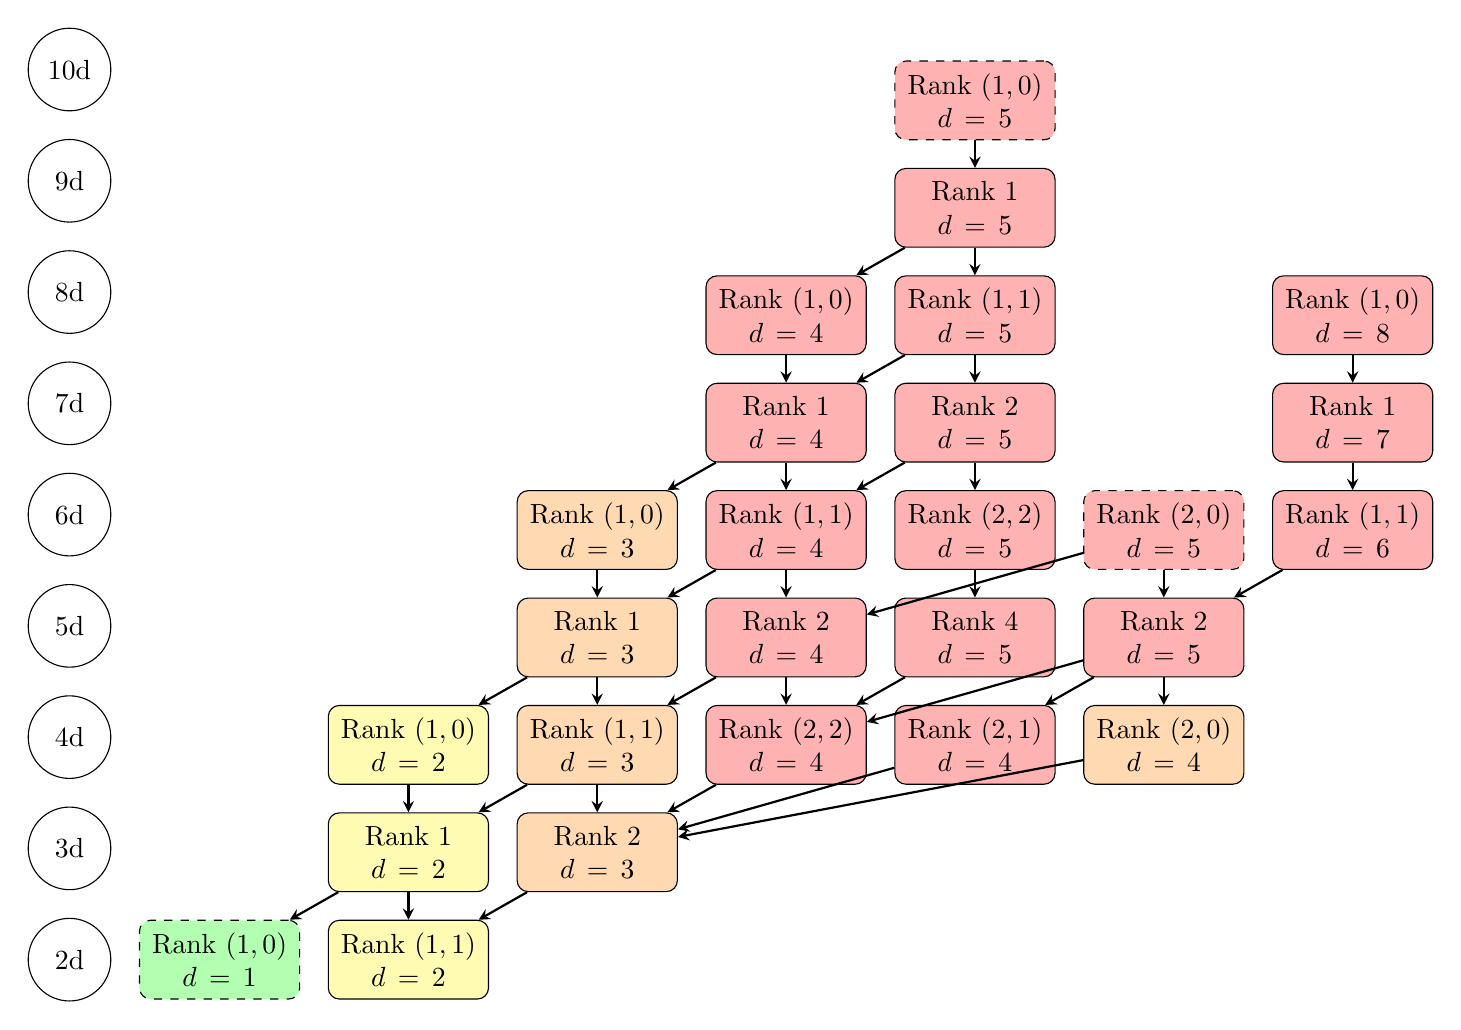
\begin{tikzpicture}[node distance=0.35cm and 0.35cm, text width=1.8cm]
\node (101) [s16chiral] {Rank $(1, 0)$ $d=5$};
\node (91) [s16, below=of 101] {Rank $1$ $d=5$};
\node (82) [s16, below=of 91] {Rank $(1, 1)$ $d=5$};
\node (81) [s16, left=of 82] {Rank $(1, 0)$ $d=4$};
\node (825) [right=of 82] {};
\node (83) [s16, right=of 825] {Rank $(1, 0)$ $d=8$};
\node (71) [s16, below=of 81] {Rank $1$ $d=4$};
\node (72) [s16, below=of 82] {Rank $2$ $d=5$};
\node (73) [s16, below=of 83] {Rank $1$ $d=7$};
\node (62) [s16, below=of 71] {Rank $(1, 1)$ $d=4$};
\node (61) [s8, left=of 62] {Rank $(1, 0)$ $d=3$};
\node (63) [s16, below=of 72] {Rank $(2, 2)$ $d=5$};
\node (64) [s16chiral, right=of 63] {Rank $(2, 0)$ $d=5$};
\node (65) [s16, below=of 73, right=of 64] {Rank $(1, 1)$ $d=6$};
\node (51) [s8, below=of 61] {Rank $1$ $d=3$};
\node (52) [s16, below=of 62] {Rank $2$ $d=4$};
\node (53) [s16, below=of 63] {Rank $4$ $d=5$};
\node (54) [s16, below=of 64] {Rank $2$ $d=5$};
\node (42) [s8, below=of 51] {Rank $(1, 1)$ $d=3$};
\node (41) [s4, left=of 42] {Rank $(1, 0)$ $d=2$};
\node (43) [s16, right=of 42] {Rank $(2, 2)$ $d=4$};
\node (44) [s16, right=of 43] {Rank $(2, 1)$ $d=4$};
\node (45) [s8, right=of 44] {Rank $(2, 0)$ $d=4$};
\node (31) [s4, below=of 41] {Rank $1$ $d=2$};
\node (32) [s8, below=of 42] {Rank $2$ $d=3$};
\node (22) [s4, below=of 31] {Rank $(1, 1)$ $d=2$};
\node (21) [s2chiral, left=of 22] {Rank $(1, 0)$ $d=1$};

\draw[arrow] (101) -- (91);
\draw[arrow] (91) -- (81);
\draw[arrow] (91) -- (82);
\draw[arrow] (81) -- (71);
\draw[arrow] (82) -- (71);
\draw[arrow] (82) -- (72);
\draw[arrow] (83) -- (73);
\draw[arrow] (71) -- (61);
\draw[arrow] (71) -- (62);
\draw[arrow] (72) -- (62);
\draw[arrow] (72) -- (63);
\draw[arrow] (73) -- (65);
\draw[arrow] (61) -- (51);
\draw[arrow] (62) -- (51);
\draw[arrow] (62) -- (52);
\draw[arrow] (63) -- (53);
\draw[arrow] (64) -- (52);
\draw[arrow] (64) -- (54);
\draw[arrow] (65) -- (54);
\draw[arrow] (51) -- (41);
\draw[arrow] (51) -- (42);
\draw[arrow] (52) -- (42);
\draw[arrow] (52) -- (43);
\draw[arrow] (53) -- (43);
\draw[arrow] (54) -- (43);
\draw[arrow] (54) -- (44);
\draw[arrow] (54) -- (45);
\draw[arrow] (41) -- (31);
\draw[arrow] (42) -- (31);
\draw[arrow] (42) -- (32);
\draw[arrow] (43) -- (32);
\draw[arrow] (44) -- (32);
\draw[arrow] (45) -- (32);
\draw[arrow] (31) -- (21);
\draw[arrow] (31) -- (22);
\draw[arrow] (32) -- (22);

\node (2d) [dimension, left=of 21] {2d};
\node (3d) [dimension, above=of 2d] {3d};
\node (4d) [dimension, above=of 3d] {4d};
\node (5d) [dimension, above=of 4d] {5d};
\node (6d) [dimension, above=of 5d] {6d};
\node (7d) [dimension, above=of 6d] {7d};
\node (8d) [dimension, above=of 7d] {8d};
\node (9d) [dimension, above=of 8d] {9d};
\node (10d) [dimension, above=of 9d] {10d};
\end{tikzpicture}
\caption{Orbits of square-zero supercharges.}
\label{fig:superchargeorbits}
\end{figure}
\end{landscape}

\section{Supersymmetric Yang--Mills theories}

In this section we construct supersymmetry action on super Yang--Mills theories. We have the following variants of the super Yang--Mills theory depending on $\dim(\Sigma)$:
\begin{itemize}
\item (16 supercharges). This theory exists in dimensions 2 through 10 and it depends on a Lie algebra $\fg$.

\item (8 supercharges). This theory exists in dimensions 2 through 6 and it depends on a Lie algebra $\fg$ together with a symplectic $\fg$-representation $U$.

\item (4 supercharges). This theory exists in dimensions 2 through 4 and it depends on a Lie algebra $\fg$ together with a $\fg$-representation $R$.

\item (2 supercharges). This theory exists in dimensions 2 through 3 and it depends on a Lie algebra $\fg$ together with an orthogonal $\fg$-representation $P$.
\end{itemize}

There are a few additional possibilities that occur in dimension 2.

\begin{itemize}
\item ($\cN_+$ supercharges, chiral supersymmetry). This theory exists in dimension 2 and depends on a Lie algebra $\fg$.

\item (4 supercharges, chiral supersymmetry). This theory exists in dimension 2 and depends on a Lie algebra $\fg$ together with a symplectic $\fg$-representation $U$.

\item (2 supercharges, chiral supersymmetry). This theory exists in dimension 2 and depends on a Lie algebra $\fg$ together with a $\fg$-representation $R$.

\item (1 supercharge, chiral supersymmetry). This theory exists in dimension 2 and depends on a Lie algebra $\fg$ together with an orthogonal $\fg$-representation $P$.
\end{itemize}

In each case the lower-dimensional theories are obtained by dimensional reduction from the theory in the highest dimension: for instance, 7d $\mc N=1$ super Yang--Mills (16 supercharges) is obtained by dimensional reduction from 10d $\mc N=(1, 0)$ super Yang--Mills. So, it will be enough to construct the supersymmetry action in these highest-dimensional theories.

\subsection{Pure super Yang--Mills theory}
\label{sect:gaugemultipletSUSY}

We begin with a description of certain pure supersymmetric Yang--Mills theories. Let $V_\RR$ be a real vector space equipped with a nondegenerate symmetric bilinear pairing and $V$ its complexification. Fix a $\ZZ/2$-graded Clifford module $\Sigma\oplus \Sigma^*\rightarrow \CC$ with the associated $\Gamma$-pairings
\[\Gamma\colon \Sym^2(\Sigma)\rightarrow V,\qquad \Gamma\colon \Sym^2(\Sigma^*)\rightarrow V\]
defined as in Appendix \ref{sect:spinors}. We make the following assumption on this setup.

\begin{assumption}
For $Q_1, Q_2, Q_3\in\Sigma$ we have
\[\rho(\Gamma(Q_1, Q_2))Q_3 + \rho(\Gamma(Q_2, Q_3))Q_1 + \rho(\Gamma(Q_3, Q_1))Q_2 = 0.\]
\label{assumption:3psi}
\end{assumption}

Explicitly, we consider the following cases:
\begin{itemize}
\item (\textbf{2d $\cN=(\cN_+, 0)$ supersymmetry}) We have $\dim(V) = 2$ and $\Sigma = S_+\otimes W$ for some complex vector space $W$ equipped with a nondegenerate symmetric bilinear pairing. Assumption \ref{assumption:3psi} is satisfied by Theorem \ref{thm:2d3psi}.

\item (\textbf{3d $\cN=1$ supersymmetry}) We have $\dim(V) = 3$ and $\Sigma = S$. Assumption \ref{assumption:3psi} is satisfied by Theorem \ref{thm:3psi}.

\item (\textbf{4d $\cN=1$ supersymmetry}) We have $\dim(V) = 4$ and $\Sigma = S_+\oplus S_-$. Assumption \ref{assumption:3psi} is satisfied by Theorem \ref{thm:3psi}.

\item (\textbf{6d $\cN=(1, 0)$ supersymmetry}) We have $\dim(V) = 6$ and $\Sigma = S_+\otimes W_+$ for a two-dimensional complex symplectic vector space $W_+$. Assumption \ref{assumption:3psi} is satisfied by Theorem \ref{thm:3psi}.

\item (\textbf{10d $\cN=(1, 0)$ supersymmetry}) We have $\dim(V) = 10$ and $\Sigma = S_+$. Assumption \ref{assumption:3psi} is satisfied by Theorem \ref{thm:3psi}.
\end{itemize}

Let $\fg$ be a Lie algebra equipped with a nondegenerate symmetric bilinear pairing. The fields of the Yang--Mills theory are as follows:
\begin{itemize}
\item A connection $A \in \Omega^1(V_\RR; \fg)$ on the trivial bundle.

\item A spinor $\lambda \in \Gamma(V_\RR; \Pi \Sigma \otimes \fg)$.

\item A ghost field $c\in\Gamma(V_\RR; \Pi\fg)$.
\end{itemize}
We also introduce their antifields $A^*\in\Omega^1(V_\RR; \Pi\fg)$, $\lambda\in\Gamma(V_\RR; \Sigma^*\otimes \fg)$ and $c^*\in\Gamma(V_\RR; \fg)$.
Let $\cE_{\rm SYM}$ denote the space of BV fields. 

Denote by $F_A = \d A + \frac{1}{2}[A\wedge A]$ the curvature of $A$ and let $\sd\d_A$ be the twisted Dirac operator obtained from $\Gamma$ (see Appendix \ref{sect:spinors}).

The BRST action is given by
\[S_{BRST}(A, \lambda) = \int_{V_\RR}\dvol \left( -\frac{1}{4} (F_A, F_A) + \frac{1}{2}(\lambda, \sd \d_A \lambda)\right).\]

We introduce gauge transformations
\[\delta A = -\d_A c,\qquad \delta \lambda = [c, \lambda],\qquad \delta c = \frac{1}{2}[c, c],\]
so that the BV action is given by
\begin{equation}
S_{\gauge} = \int_{V_\RR}\dvol \left( -\frac{1}{4} (F_A, F_A) + \frac{1}{2}(\lambda, \sd\d_A \lambda) + (\d_A c, A^*) + ([c, \lambda], \lambda^*) + \frac{1}{2}([c, c], c^*)\right).
\label{eq:YMBVaction}
\end{equation}

To simplify the notation, the pairing on $\fg$ from now on will be implicit.

The Poincar\'e group acts, in the sense of Definition \ref{group_action_def}, on Yang--Mills theory on $\RR^n$. Indeed, there is an obvious Poincar\'e action on fields where we use that $\Sigma$ is a representation of $\Spin(V_\RR)$. The corresponding Hamiltonian is given by
\begin{equation}
I_{\gauge}^{(1)}(v) = \int_{V_\RR}\dvol\left( (L_{v}A, A^*) - (v.\lambda, \lambda^*) - (v.c)c^*\right),
\label{eq:YMPoincareaction}
\end{equation}
for $v\in\mf{iso}(V)$, where $v.\lambda$ contains both a derivative and the $\so(V)$ action on $\Sigma$.

We will now construct an elliptic $L_\infty$ action of the super Lie algebra $\mf{A}$ on the theory. 
Following Definition \ref{infinitesimal_action_def}, we have to prescribe a collection of functionals $I_{\gauge}^{(1)}, I_{\gauge}^{(2)}, \dots$, where $I_{\gauge}^{(k)}\colon \mf{A}^{\otimes k}\rightarrow \oloc(\cE)$, satisfying the classical master equation. The supersymmetry action we construct will extend the Poincar\'{e} action from \eqref{eq:YMPoincareaction}, so we just have to specify the values of $I_{\gauge}^{(k)}$ on the supersymmetry generators in $\Sigma$. The action of supersymmetry is given by a linear and quadratic functionals
\begin{align*}
I_{\gauge}^{(1)}(Q) &= \int_{V_\RR}\dvol\left( -(\Gamma(Q, \lambda), A^*) + \frac{1}{2}(\rho(F_A)Q, \lambda^*)\right) \\
I_{\gauge}^{(2)}(Q_1, Q_2) &= \int_{V_\RR}\dvol\left( \frac{1}{4}(\Gamma(Q_1, Q_2), \Gamma(\lambda^*, \lambda^*)) - \frac{1}{2}(Q_1, \lambda^*)(Q_2, \lambda^*) - \iota_{\Gamma(Q_1, Q_2)} A c^*\right).
\end{align*}

The following theorem summarizes the fact that super Yang-Mills theory is indeed supersymmetric in the sense of Definition \ref{dfn: super}. 

\begin{thm}\label{thm:gaugemultipletSUSY}
The functional $\fS_{\gauge} = S_{\gauge} + I_{\gauge}^{(1)} + I_{\gauge}^{(2)} \in C^\bu(\mf{A}, \oloc(\cE_{\rm SYM}))$ defines satisfies the classical master equation
\[\d_{CE} \fS_{\gauge} + \frac{1}{2}\{\fS_{\gauge}, \fS_{\gauge}\} = 0.\]
Thus, $\fS_{\gauge}$ defines an elliptic $L_\infty$ action of the super Lie algebra $\fA$ on super Yang-Mills theory and so super Yang-Mills theory is supersymmetric.  
\end{thm}

The rest of the section will be devoted to the proof of the above theorem. The classical master equation decomposes into the following equations:
\begin{align*}
\{S_{\gauge}, I_{\gauge}^{(1)}\} &= 0 \\
\{S_{\gauge}, I_{\gauge}^{(2)}\} + \d_{CE} I_{\gauge}^{(1)} + \frac{1}{2}\{I_{\gauge}^{(1)}, I_{\gauge}^{(1)}\} &= 0 \\
\d_{CE} I_{\gauge}^{(2)} + \{I_{\gauge}^{(1)}, I_{\gauge}^{(2)}\} &= 0 \\
\{I_{\gauge}^{(2)}, I_{\gauge}^{(2)}\} &= 0.
\end{align*}

Note that the last equation is automatically satisfied since $I_{\gauge}^{(2)}$ is independent of $\lambda$ and $c$. The rest of the claims will be proved in a sequence of Lemmas. To simplify the expressions, we drop the integrals.

\begin{lemma}
One has $\{S_{\gauge}, I_{\gauge}^{(1)}(Q)\} = 0$.
\label{lm:gaugemultiplet1}
\end{lemma}
\begin{proof}
Let us decompose $S_{\gauge} = \sum_{i=1}^5 S_{\gauge}^i$ into individual summands.

The first term gives
\begin{align*}
\{S_{\gauge}^1, I_{\gauge}^{(1)}(Q)\} &= -\frac{1}{2} (\d_A \Gamma(Q, \lambda), F_A)\\
&= -\frac{1}{2}(-1)^{n-1} (\ast \d_A \ast F_A, \Gamma(Q, \lambda)).
\end{align*}

The second term gives
\begin{align*}
\{S_{\gauge}^2, I_{\gauge}^{(1)}(Q)\} &= -\frac{1}{2}(\lambda, \rho(\Gamma(Q, \lambda))\lambda) + \frac{1}{2}(\rho(F_A) Q, \sd{\d}_A\lambda) \\
&= -\frac{1}{2}(\Gamma(Q, \lambda), \Gamma(\lambda, \lambda))  - \frac{1}{2}(\lambda, \sd{\d}_A(\rho(F_A) Q)) \\
&= -\frac{1}{2}(\Gamma(Q, \lambda), \Gamma(\lambda, \lambda)) - \frac{1}{2} (-1)^n (\lambda, \rho(\ast \d_A\ast F_A) Q),
\end{align*}
where we have used Proposition \ref{prop:cliffordactionproperty3} and the Bianchi identity in the last line.

By \eqref{eq:Gammaspinorpairing} and Assumption \ref{assumption:3psi} we have $(\Gamma(Q, \lambda), \Gamma(\lambda, \lambda)) = 0$, so $\{S_{\gauge}^1 + S_{\gauge}^2, I_{\gauge}^{(1)}(Q)\} = 0$.

Finally, $\{S_{\gauge}^3 + S_{\gauge}^4 + S_{\gauge}^5, I_{\gauge}^{(1)}(Q)\} = 0$ due to gauge-invariance of $I^{(1)}(Q)$.
\end{proof}

\begin{remark}
The previous Lemma expresses the fact that the pure super Yang--Mills action is supersymmetric; our proof essentially follows \cite{BaezHuerta}.
\end{remark}

\begin{lemma}
One has
\[\{S_{\gauge}, I_{\gauge}^{(2)}\} + \d_{CE} I_{\gauge}^{(1)} + \frac{1}{2}\{I_{\gauge}^{(1)}, I_{\gauge}^{(1)}\} = 0.\]
\label{lm:gaugemultiplet2}
\end{lemma}
\begin{proof}
Evaluating the equation
\[\{S_{\gauge}, I_{\gauge}^{(2)}\} + \d_{CE} I_{\gauge}^{(1)} + \frac{1}{2}\{I_{\gauge}^{(1)}, I_{\gauge}^{(1)}\} = 0\]
on $v_1, v_2\in \mf{iso}(V)$, the claim reduces to the fact that \eqref{eq:YMPoincareaction} defines a strict Lie action. Evaluating it on $v\in\mf{iso}(V)$ and $Q\in\Sigma$, the claim reduces to the fact that $I_{\gauge}^{(1)}$ is Poincar\'{e}-invariant. So, the only nontrivial check is for $Q_1,Q_2\in\Sigma$.

The individual terms are
\begin{align*}
\frac{1}{2}\{I_{\gauge}^{(1)}, I_{\gauge}^{(1)}\}(Q_1, Q_2) = &-\{I_{\gauge}^{(1)}(Q_1), I_{\gauge}^{(1)}(Q_2)\} \\
= &-\frac{1}{2}(\rho(\d_A \Gamma(Q_1, \lambda)) Q_2, \lambda^*) + \frac{1}{2}(\Gamma(Q_2, \rho(F_A)Q_1), A^*) \\
&-\frac{1}{2}(\rho(\d_A \Gamma(Q_2, \lambda)) Q_1, \lambda^*) + \frac{1}{2}(\Gamma(Q_1, \rho(F_A)Q_2), A^*),
\end{align*}
\begin{align*}
(\d_{CE} I_{\gauge}^{(1)})(Q_1, Q_2) &= I_{\gauge}^{(1)}(\Gamma(Q_1, Q_2)) \\
&= (L_{\Gamma(Q_1, Q_2)}(A), A^*) -(\Gamma(Q_1, Q_2).\lambda, \lambda^*) - (\Gamma(Q_1, Q_2).c) c^*
\end{align*}
and
\begin{align*}
\{S_{\gauge}, I_{\gauge}^{(2)}(Q_1, Q_2)\} = &-\frac{1}{2}(Q_2, \lambda^*)(Q_1, \sd{\d}_A \lambda + [c, \lambda^*]) - \frac{1}{2}(Q_1, \lambda^*)(Q_2, \sd{\d}_A \lambda + [c, \lambda^*]) \\
&+\frac{1}{2}(\Gamma(Q_1, Q_2), \Gamma(\lambda^*, \sd{\d}_A \lambda + [c, \lambda^*])) + \iota_{\Gamma(Q_1, Q_2)}(\d_A c) c^* - (\d_A\iota_{\Gamma(Q_1, Q_2)} A, A^*) \\
&+ ([\lambda, \iota_{\Gamma(Q_1, Q_2)}A], \lambda^*) - [\iota_{\Gamma(Q_1, Q_2)} A, c] c^*
\end{align*}
The total coefficient in front of $A^*$ is
\[\frac{1}{2}\Gamma(Q_1, \rho(F_A)Q_2) + \frac{1}{2}\Gamma(Q_2, \rho(F_A) Q_1) + L_{\Gamma(Q_1, Q_2)} A - \d_A \iota_{\Gamma(Q_1, Q_2)} A.\]
Using Proposition \ref{prop:cliffordactionproperty1} we get that the sum of the first two terms is $-\iota_{\Gamma(Q_1, Q_2)}F_A$ which cancels the last two terms.

The total coefficient in front of $c^*$ is
\[-\Gamma(Q_1, Q_2).c + \iota_{\Gamma(Q_1, Q_2)}(\d_A c) - [\iota_{\Gamma(Q_1, Q_2)} A, c] = 0.\]

The total coefficient in front of $\lambda^*$ is
\begin{align*}
&-\frac{1}{2}\rho(\d_A \Gamma(Q_1, \lambda))Q_2 -\frac{1}{2}\rho(\d_A \Gamma(Q_2, \lambda))Q_1 - \Gamma(Q_1, Q_2).\lambda \\
&+ \frac{1}{2}\rho(\Gamma(Q_1, Q_2))\sd{\d}_A\lambda - \frac{1}{2}(Q_2, \sd{\d}_A\lambda) Q_1 -\frac{1}{2}(Q_1, \sd{\d}_A\lambda) Q_2 + [\lambda, (\Gamma(Q_1, Q_2), A)]
\end{align*}
Using Proposition \ref{prop:cliffordactionproperty2} the first, second, fifth and sixth terms combine to
\[-\frac{1}{2} \sd{\d}_A\rho(\Gamma(Q_1, \lambda))Q_2 - \frac{1}{2} \sd{\d}_A\rho(\Gamma(Q_2, \lambda)) Q_1\]
which is equal to $\frac{1}{2} \sd{\d}_A \rho(\Gamma(Q_1, Q_2))\lambda$ by Assumption \ref{assumption:3psi}. Using the Clifford relation this term cancels the rest of the terms.
\end{proof}

Evaluating the equation
\[\d_{CE} I_{\gauge}^{(2)} + \{I_{\gauge}^{(1)}, I_{\gauge}^{(2)}\} = 0\]
on $v_1, v_2, v_3\in\mf{iso}(V)$ or on $v_1, v_2\in\mf{iso}(V)$ and $Q\in\Sigma$ we automatically get zero. Evaluating it on $v\in\mf{iso}(V)$ and $Q_1, Q_2\in\Sigma$ we get Poincar\'{e}-invariance of $I_{\gauge}^{(2)}$.

\begin{lemma}
\[\{I_{\gauge}^{(1)}, I_{\gauge}^{(2)}\}(Q_1, Q_2, Q_3) = 0\]
for every $Q_1, Q_2, Q_3\in\Sigma$.
\label{lm:gaugemultiplet3}
\end{lemma}
\begin{proof}
We have
\begin{align*}
\{I_{\gauge}^{(1)}(Q_1), I_{\gauge}^{(2)}(Q_2, Q_3)\} = &-\iota_{\Gamma(Q_2, Q_3)}\Gamma(Q_1, \lambda) c^* - \frac{1}{2} (\Gamma(Q_2, Q_3), \Gamma(\rho(A^*) Q_1, \lambda^*)) \\
&+ \frac{1}{2}(Q_2, \rho(A^*)Q_1)(Q_3, \lambda^*) + \frac{1}{2}(Q_3, \rho(A^*) Q_1)(Q_2, \lambda^*).
\end{align*}

$\{I_{\gauge}^{(1)}, I_{\gauge}^{(2)}\}(Q_1, Q_2, Q_3)$ is obtained by cyclically symmetrizing the above expression. By Assumption \ref{assumption:3psi} the cyclic symmetrization of the term with $c^*$ is zero. The Clifford relation implies that
\begin{align*}
\frac{1}{2} (\Gamma(Q_2, Q_3), \Gamma(\rho(A^*) Q_1, \lambda^*)) &= -\frac{1}{2}(\Gamma(Q_2, Q_3), \Gamma(\rho(A^*)\lambda^*, Q_1)) + (\Gamma(Q_2, Q_3), A^*) (Q_1, \lambda^*) \\
&= -\frac{1}{2}(\rho(\Gamma(Q_2, Q_3)) Q_1, \rho(A^*)\lambda^*) + (\Gamma(Q_2, Q_3), A^*) (Q_1, \lambda^*).
\end{align*}
Therefore, again using Assumption \ref{assumption:3psi} we see that the cyclic symmetrization of the terms with $A^*$ vanishes.
\end{proof}

\begin{comment}
\pavel{This might go in the coupling section.}
We can deduce supersymmetry for other super Yang-Mills theories using dimensional reduction, specifically Proposition \ref{dim_red_SUSY_prop}.
\begin{corollary}
Let $n$ be one of the special dimensions $3,4,6$ or 10, and choose $m < n$.  Let $\Sigma'$ be the $\so(m)$ representation obtained by restriction of the $\so(n)$ representation $\Sigma$.  Then the super Poincar\'e algebra
\[\mf A' = \mf{iso}(m) \oplus \Pi \Sigma',\]
obtained by restricting the $n$-dimensional super Poincar\'e algebra associated to $\Sigma$, acts on the $m$-dimensional super Yang-Mills theory $\mf L'$ with matter representation $\Sigma'$.
\end{corollary}

\begin{proof}
This follows immediately by applying Proposition \ref{dim_red_SUSY_prop} to the $\mf A$-supersymmetric theory $\mf L$ on $\RR^n$.
\end{proof}

\begin{remark}
We can further include the action of at least a subalgebra of the algebra of R-symmetries in each example. \chris{quantify which}
\end{remark}
\end{comment}

\subsection{Matter multiplet}
\label{sect:mattermultipletSUSY}

In this section we describe the coupling of super Yang--Mills theory to matter valued in a $\fg$-representation $P$, i.e. the supersymmetric gauged linear $\sigma$-models. Our description of the supersymmetry of the matter multiplet is inspired by the presentation of the supersymmetric nonlinear $\sigma$-models in \cite[Chapter 3]{DeligneFreed}.

Consider as before $V_\RR$ and a Clifford module $\Sigma\oplus \Sigma^*$ satisfying Assumption \ref{assumption:3psi}. In addition, fix a real associative algebra $A_\RR$ equipped with an antiinvolution $\sigma$ as in Section \ref{sect:divisionalgebras} and denote its complexification by $A$. Suppose $\Sigma\oplus \Sigma^*$ carries a compatible right $A$-module structure. Let $(-, -)^A\colon \Sigma\otimes \Sigma^*\rightarrow A$ be the correspoding $A$-valued pairing given by Lemma \ref{lm:extendpairing}. We make the following additional assumption.

\begin{assumption}
For $Q_1, Q_2\in\Sigma$ and $Q_3\in\Sigma^*$ we have
\[Q_1(Q_2, Q_3)^A + Q_2(Q_1, Q_3)^A = \rho(\Gamma(Q_1, Q_2))Q_3.\]
\label{assumption:matter3psi}
\end{assumption}

Explicitly, we consider the following cases:
\begin{itemize}
\item (\textbf{2d $\cN=(1, 0)$ supersymmetry}) $A_\RR = \RR$. Assumption \ref{assumption:matter3psi} is satisfied by Theorem \ref{thm:2dmatter3psi}.

\item (\textbf{2d $\cN=(2, 0)$ supersymmetry}) $A_\RR = \CC$. Assumption \ref{assumption:matter3psi} is satisfied by Theorem \ref{thm:2dmatter3psi}.

\item (\textbf{2d $\cN=(4, 0)$ supersymmetry}) $A_\RR = \mathbb{H}$. Assumption \ref{assumption:matter3psi} is satisfied by Theorem \ref{thm:2dmatter3psi}.

\item (\textbf{3d $\cN=1$ supersymmetry}) $A_\RR = \RR$. Assumption \ref{assumption:matter3psi} is satisfied by Theorem \ref{thm:matter3psi}.

\item (\textbf{4d $\cN=1$ supersymmetry}) $A_\RR = \CC$. Assumption \ref{assumption:matter3psi} is satisfied by Theorem \ref{thm:matter3psi}.

\item (\textbf{6d $\cN=(1, 0)$ supersymmetry}) $A_\RR = \mathbb{H}$. Assumption \ref{assumption:matter3psi} is satisfied by Theorem \ref{thm:matter3psi}.
\end{itemize}

Let $P$ be a left $A$-module equipped with a $\CC$-valued nondegenerate symmetric bilinear pairing such that
\[(av, w) = (v, \sigma(a)w).\]
Moreover, assume $P$ carries a $\fg$-action commuting with the $A$-module structure and preserving the bilinear pairing. Explicitly, for $A_\RR=\RR, \CC, \mathbb{H}$ we get the following data:
\begin{itemize}
\item $A_\RR=\RR$, so $A=\CC$. We are looking for a $\fg$-representation $P$ equipped with a nondegenerate symmetric bilinear pairing.

\item $A_\RR=\CC$, so $A=\CC[x]/(x^2+1)$. A left $A$-module $P$ splits as $P=P_+\oplus P_-$, where $x$ acts as $\pm i$ on $P_{\pm}$. Note that with respect to the right $A$-action $x$ acts as $\mp i$ on $P_{\pm}$. So, the symmetric bilinear pairing identifies $P_+\cong P_-^*$. In other words, the data boils down to a $\fg$-representation $R$, so that $P = R\oplus R^*$.

\item $A_\RR=\mathbb{H}$, so $A=\eend(W_+)$. A left $A$-module is necessarily of the form $P\cong W_+\otimes U$, where $A$ just acts on $W_+$. Compatibility of the orthogonal pairing on $P$ with the $A$-action implies that it is given by a product of the symplectic pairing on $W_+$ and a symplectic pairing on $U$. So, the data boils down a symplectic $\fg$-representation $U$.
\end{itemize}

We are going to construct a theory on $V_\RR$ describing a matter multiplet valued in $P$. The BRST fields are given as follows:
\begin{itemize}
\item a scalar $\phi\in\Gamma(V_\RR; P)$;
\item a spinor $\psi\in\Gamma(V_\RR; \Pi \Sigma^*\otimes_A P)$.
\end{itemize}
As usual, we denote the antifields by $\phi^*\in\Gamma(V_\RR; \Pi P)$ and $\psi^*\in\Gamma(V_\RR; \Sigma\otimes_A P)$.

We extend the pairings on $P$ and between $\Sigma$ and $\Sigma^*$ to a pairing between $\Sigma\otimes_A P$ and $\Sigma^*\otimes_A P$ in the following way. Given $\sum_i \tilde{s}_i\otimes v_i\in \Sigma^*\otimes_A P$ and $\sum_j s_j\otimes w_j\in\Sigma\otimes_A P$, their pairing is
\begin{equation}
\sum_{i, j} \Re((v_i, w_j)^A (s_j, \tilde{s}_i)^A),
\label{eq:spinorialmatterpairing}
\end{equation}
where we extend both pairings to $A$-valued pairings using Lemma \ref{lm:extendpairing}. We may also extend the $\Gamma$-pairing to a map
\[\Gamma\colon \Sym^2(\Sigma^*\otimes_A P)\rightarrow V\]
defined by the property
\[(v, \Gamma(\psi_1, \psi_2)) = (\psi_1, \rho(v) \psi_2),\qquad v\in V,\ \psi_i\in \Sigma^*\otimes_A P.\]

The BV action for the matter multiplet is
\[
S_{\matter} = \int_{V_\RR} \dvol \left(\frac{1}{2}  (\d_A \phi, \d_A \phi) + (\psi , \sd \d_A \psi) + 2 (\lambda\phi, \psi) + (c\psi, \psi^*) - (c\phi, \phi^*)\right),
\]
where we use the pairing \eqref{eq:spinorialmatterpairing} in the second term.

It is Poincar\'{e}-invariant with the corresponding Hamiltonian
\begin{equation}
I_{\matter}^{(1)}(v) = \int_{V_\RR}\dvol\left( (L_{v}A, \phi^*) - (v.\psi, \psi^*)\right),
\label{eq:matterPoincareaction}
\end{equation}
for $v\in\mf{iso}(V)$.

The action of supersymmetry is given by a linear and quadratic functional:
\begin{align*}
I_{\matter}^{(1)} (Q) & = \int_{V_\RR}\dvol\left( ((Q, \psi), \phi^*) + \frac{1}{2}(\rho(\d_A \phi) Q, \psi^*)\right) \\
I_{\matter}^{(2)} (Q_1 , Q_2) & = \frac{1}{4}\int_{V_\RR} \dvol(\Gamma(Q_1, Q_2) , \Gamma(\psi^*, \psi^*))
\end{align*}
where $Q, Q_1,Q_2 \in \Sigma$.

We consider the full action of the super Yang--Mills theory
\[S_{\BV} = S_{\gauge} + S_{\matter}\]
together with a supersymmetry action functionals
\[I^{(1)} = I^{(1)}_{\gauge} + I^{(1)}_{\matter},\qquad I^{(2)} = I^{(2)}_{\gauge} + I^{(2)}_{\matter}.\]

The following result states that these functionals encode an off-shell action of the supersymmetry algebra.

\begin{thm}
The functional $\fS = S_{\BV} + I_{\BV}^{(1)} + I_{\BV}^{(2)}$ satisfies the classical master equation
\begin{equation}
\label{CMEYM}
\d_{CE} \fS + \frac{1}{2} \{\fS, \fS\} = 0 .
\end{equation}
\label{thm:YMSUSY}
\end{thm}

The rest of this section is devoted to the proof of Theorem \ref{thm:YMSUSY}. The classical master equation \eqref{CMEYM} decomposes into a sequence of equations
\begin{equation}
\label{CMEYM2}
\begin{array}{rrrrrr}
\{S_{\BV} , I^{(1)}\} & = & 0 \\ 
\{S_{\matter}, I^{(2)}\} + \d_{CE} I_{\matter}^{(1)} + \{I_{\gauge}^{(1)}, I_{\matter}^{(1)}\} + \frac{1}{2} \{I_{\matter}^{(1)}, I_{\matter}^{(1)}\} & = & 0 \\
\d_{CE} I_{\matter}^{(2)} + \{I_{\matter}^{(1)}, I_{\matter}^{(2)}\} & =& 0 \\
\{I_{\matter}^{(2)}, I_{\matter}^{(2)}\} & =& 0
\end{array}
\end{equation}

The last equation is automatically satisfied since $I^{(2)}$ is independent of the fields $\phi, \psi, A, \lambda$.

The first equation in \eqref{CMEYM2} states that the classical action is supersymmetric.

\begin{lemma} \label{lem:YM1}
One has $\{S_{\BV}, I^{(1)}\} (Q) = 0$ for all $Q \in \Sigma$. 
\end{lemma}
\begin{proof}
Let us decompose $S_{\matter}=\sum_{i=1}^5 S_{\matter}^i$ into individual summands.

The first term gives
\begin{align*}
\{S_{\matter}^1, I^{(1)}(Q)\} &= -(\d_A\phi, \d_A(Q, \psi)) + (\Gamma(Q, \lambda)\phi, \d_A\phi) \\
&= \d_A^* \d_A\phi (Q, \psi) + (\Gamma(Q, \lambda)\phi, \d_A\phi).
\end{align*}

The second term gives
\begin{align*}
\{S_{\matter}^2, I^{(1)}(Q)\} &= -(\psi, \sd \d_A \rho(\d_A \phi) Q) - (\psi, \rho(\Gamma(Q, \lambda))\psi) \\
&= -(\psi, \rho(F_A) Q)\phi - \d_A^*\d_A \phi(\psi, Q) - (\psi, \rho(\Gamma(Q, \lambda))\psi),
\end{align*}
where we have used Proposition \ref{prop:cliffordactionproperty3} in the second line.

The third term gives
\begin{align*}
\{S_{\matter}^3, I^{(1)}(Q)\} &= ((\rho(F_A)Q) \phi, \psi) + 2(\lambda(Q, \psi), \psi) - (\lambda\phi, \rho(\d_A \phi) Q) \\
&= ((\rho(F_A)Q) \phi, \psi) + (\rho(\Gamma(Q, \lambda))\psi, \psi) - (\Gamma(\lambda\phi, Q), \d_A \phi),
\end{align*}
where we have used Assumption \ref{assumption:matter3psi} in the middle term and \eqref{eq:Gammaspinorpairing} in the last term. It is then obvious that
\[\{S_{\matter}^1 + S_{\matter}^2 + S_{\matter}^3, I^{(1)}(Q)\} = 0.\]

Finally, the terms $\{S_{\matter}^4 + S_{\matter}^5 + S_{\gauge}^3, I^{(1)}(Q)\}$ are zero due to gauge-invariance of $I^{(1)}(Q)$ while the rest of the terms are zero by Lemma \ref{lm:gaugemultiplet1}.
\end{proof}

Next, we move on to the second equation in \eqref{CMEYM2}.

\begin{lemma} 
One has
\begin{equation}\label{CMEYM3}
\{S_{\matter}, I^{(2)}\} + \d_{CE} I_{\matter}^{(1)} + \{I_{\gauge}^{(1)}, I_{\matter}^{(1)}\} + \frac{1}{2} \{I_{\matter}^{(1)}, I_{\matter}^{(1)}\} = 0 .
\end{equation}
\end{lemma}
\begin{proof}
Evaluating expression \eqref{CMEYM3} on $v_1,v_2 \in \mf{iso}(V)$ reduces to the claim that \eqref{eq:matterPoincareaction} defines a strict Lie action. Evaluating on $v \in \mf{iso}(V)$ and $Q \in \Sigma$, the claim reduces to the fact that $I^{(1)}$ is Poincar\'{e}-invariant. So, the only nontrivial term to check is the evaluation on $Q_1,Q_2 \in \Sigma$. 

The individual terms are:
\begin{align*}
\frac{1}{2}\{I_{\matter}^{(1)}, I_{\matter}^{(1)}\}(Q_1, Q_2) =& -\{I_{\matter}^{(1)}(Q_1), I_{\matter}^{(1)}(Q_2)\} \\
=&-\frac{1}{2}(Q_1, \rho(\d_A \phi) Q_2)\phi^* - \frac{1}{2}(Q_2, \rho(\d_A \phi)Q_1)\phi^* \\ &  +\frac{1}{2}(\rho(\d(Q_1,\psi))Q_2, \psi^*) +\frac{1}{2} (\rho(\d(Q_2, \psi)) Q_1, \psi^*),
\end{align*}

\begin{align*}
\{I_{\gauge}^{(1)}, I_{\matter}^{(1)}\}(Q_1, Q_2) = &-\{I_{\gauge}^{(1)}(Q_1), I_{\matter}^{(1)}(Q_2)\} - \{I_{\gauge}^{(1)}(Q_2), I_{\matter}^{(1)}(Q_1)\} \\
=& -\frac{1}{2}(\rho(\Gamma(Q_1, \lambda))(\phi Q_2), \psi^*) - \frac{1}{2}(\rho(\Gamma(Q_2, \lambda))(\phi Q_1), \psi^*),
\end{align*}

\[
(\d_{CE}I_{\matter}^{(1)})(Q_1,Q_2) = L_{\Gamma(Q_1,Q_2)} (\phi)\phi^* - (\Gamma(Q_1,Q_2).\psi, \psi^*),
\]

and
\[
\{S_{\matter}, I^{(2)}(Q_1,Q_2)\} =  \frac{1}{2} \Gamma(Q_1,Q_2) \Gamma(\psi^*, \sd \d_A \psi - 2 \lambda\phi + c\psi^*) - ((\iota_{\Gamma(Q_1, Q_2)} A)\psi, \psi^*) + ((\iota_{\Gamma(Q_1, Q_2)} A)\phi, \phi^*)
\]

We first collect all terms in equation \eqref{CMEYM3} proportional to $\phi^*$:
\[
-\frac{1}{2} (Q_1, \rho(\d_A\phi) Q_2) - \frac{1}{2} (Q_2, \rho(\d_A \phi) Q_1) + L_{\Gamma(Q_1,Q_2)} \phi + (\iota_{\Gamma(Q_1, Q_2)} A)\phi.
\]

By \eqref{eq:Gammaspinorpairing} we observe that the first two terms cancel with the last two terms.

Next, we collect all terms in equation \eqref{CMEYM3} containing $\psi^*$ and $\psi$:
\begin{equation}\label{psistar}
\frac{1}{2} \sd \d_A Q_2(Q_1 \psi)^A + \frac{1}{2} \sd \d_A Q_1(Q_2, \partial_i\psi)^A - \Gamma(Q_1,Q_2) . \psi + \frac{1}{2} \rho(\Gamma(Q_1,Q_2)) \sd \d_A \psi - (\iota_{\Gamma(Q_1, Q_2)} A)\psi.
\end{equation}
Applying Assumption \ref{assumption:matter3psi} to $Q_3 = \psi$, the first two terms become $\frac{1}{2} \sd \d_A \rho(\Gamma(Q_1,Q_2) \psi)$. 
Finally, by the Clifford identity the sum of this term with the fourth term in \eqref{psistar} is precisely $\iota_{\Gamma(Q_1,Q_2)}\d_A \psi$ which cancels the remaining terms.
\end{proof}

\begin{lemma}
\[\{I_{\matter}^{(1)}, I_{\matter}^{(2)}\}(Q_1, Q_2, Q_3) = 0\]
for every $Q_1, Q_2, Q_3\in \Sigma$.
\end{lemma}
\begin{proof}
We have
\begin{align*}
\{I_{\matter}^{(1)}(Q_1), I_{\matter}^{(2)}(Q_2, Q_3)\} & = \frac{1}{2} (\Gamma(Q_2, Q_3), \Gamma(\psi^*, \phi^* Q_1)) \\ & = (\psi^*, \phi^* \rho(\Gamma(Q_2,Q_3)) Q_1)  .
\end{align*}
The expression
$\{I_{\matter}^{(1)}, I_{\matter}^{(2)}\}(Q_1,Q_2,Q_3)$ is obtained by cyclically symmetrizing the above expression. By Assumption \ref{assumption:3psi} the cyclic symmetrization is identically zero.
\end{proof}

\part{A Catalogue of Twists}

\section{Dimension 10}

The 10-dimensional supersymmetry algebra has odd part $\Sigma\cong S_+\otimes W_+\oplus S_-\otimes W_-$, where $S_+, S_-$ are the 16-dimensional semi-spin representations of $\Spin(10)$, and where $W_+$ and $W_-$ are complex vector spaces equipped with a nondegenerate symmetric bilinear pairing. There are Yang--Mills theories with $\cN=(1, 0)$ or $\cN=(0, 1)$ supersymmetries. We concentrate on the first case, the second case being identical. So, we fix $W_+=\CC$ and $W_- = 0$.

\subsection{$\cN=(1, 0)$ super Yang--Mills theory}

Let $\fg$ be a complex Lie algebra equipped with a symmetric bilinear invariant nondegenerate pairing. We consider $\cN=(1, 0)$ super Yang--Mills theory on $\RR^{10}$, where $\fg$ is the complexified Lie algebra of the gauge group.

The 10d $\cN=(1, 0)$ supersymmetry algebra admits a unique twist:
\begin{itemize}
\item A square-zero supercharge $Q\neq 0\in\Sigma$ has 5 invariant directions and does not admit a compatible homomorphism $\alpha$. So, it gives rise to a $\ZZ/2$-graded holomorphic theory. A way to construct such a supercharge is to choose a complex structure on $\RR^{10}$ together with complex half-density whose square is a holomorphic volume form $\Omega\in\Omega^{5, 0}(\CC^5)$. Such a supercharge is stabilized by $\SU(5)\subset \Spin(10)$.
\end{itemize}

We will now fix a nonzero square-zero supercharge $Q$ and rewrite the fields and the action in terms of the Calabi--Yau structure. Let $\omega\in\Omega^{1, 1}(\CC^5)$ be the K\"ahler form, $\Omega\in\Omega^{5, 0}(\CC^5)$ the holomorphic volume form and $\Lambda\colon \Omega^{p+1, q+1}(\CC^5)\rightarrow \Omega^{p, q}(\CC^5)$ the dual Lefschetz operator. The vector representation decomposes as
\[\Omega^1(\CC^5)\cong \Omega^{1, 0}(\CC^5)\oplus \Omega^{0, 1}(\CC^5),\]
the semi-spin representation $S_+$ decomposes as
\[\Omega^0(\CC^5; S_+)\cong \Omega^{1, 0}(\CC^5)\oplus \Omega^{0, 2}(\CC^5)\oplus \Omega^0(\CC^5)\]
and the semi-spin representation $S_-$ decomposes as
\[\Omega^0(\CC^5; S_-)\cong \Omega^{0, 1}(\CC^5)\oplus \Omega^{2, 0}(\CC^5)\oplus \Omega^0(\CC^5).\]
Under this decomposition the scalar pairing $S_+\otimes S_-\rightarrow \CC$ corresponds to the wedge product of individual components post-composed with $\Lambda$. Under the above decomposition the Clifford multiplication of a vector $A = A_{1, 0} + A_{0, 1}$ and a spinor $\lambda = \psi + B + \chi\in S_+$ is given by
\[\rho(A)\lambda = (A_{0, 1}\chi + \Lambda(A_{1, 0}\wedge B), A_{1, 0}\wedge \psi + \ast(A_{0, 1}\wedge B\wedge\Omega), \Lambda(A_{0, 1}\wedge \psi))\in S_-.\]

\vspace{-10pt}
\paragraph{Fields:} The BRST fields are given by:
\begin{itemize}
\item Gauge fields $A_{1, 0}\in\Omega^{1, 0}(\CC^5; \gg)$, $A_{0, 1}\in\Omega^{0, 1}(\CC^5; \gg)$.
\item Fermions $\psi\in\Omega^{1, 0}(\CC^5; \Pi\gg)$, $B\in\Omega^{0, 2}(\CC^5; \Pi\gg)$, $\chi\in\Omega^0(\CC^5; \Pi\gg)$.
\item A ghost field $c\in\Omega^0(\CC^5; \Pi\gg)$.
\end{itemize}
We denote their antifields by $A_{1, 0}^*, A_{0, 1}^*, \psi^*, B^*, \chi^*, c^*$.

The BV action of the theory is obtained from \eqref{eq:YMBVaction} by decomposing it in terms of the above fields. We will need an expression for the Hodge star operator on K\"{a}hler manifolds, see \cite[Proposition 1.2.31]{Huybrechts}.

\begin{prop}
Let $(M, \omega)$ be a K\"{a}hler $d$-fold and decompose
\[\Omega^2(M) = \Omega^{2, 0}(M)\oplus \Omega^{0, 2}(M)\oplus (\CC\omega\oplus \Omega^{1, 1}_\perp(M)).\]
Then
\begin{enumerate}
\item The spaces $\Omega^{2, 0}(M)\oplus \Omega^{0, 2}(M)$, $\CC\omega$ and $\Omega^{1, 1}_\perp(M)$ are mutually orthogonal.

\item For a form $\alpha\in\Omega^{2, 0}(M)\oplus \Omega^{0, 2}(M)$ we have
\[\ast \alpha = \frac{1}{(d-2)!} \alpha\wedge \omega^{d-2}.\]

\item For $\alpha\in \Omega^{1, 1}_\perp(M)$ we have
\[\ast\alpha = -\frac{1}{(d-2)!} \alpha\wedge \omega^{d-2}.\]

\item For $\alpha\in\CC\omega$ we have
\[\ast \alpha = \frac{1}{(d-1)!} \alpha\wedge \omega^{d-2}.\]
\end{enumerate}
\end{prop}

\begin{corollary}
Let $M$ be a K\"{a}hler $d$-fold and $F = F_{2, 0} + F_{1, 1} + F_{0, 2}$ a two-form. Then
\[F\wedge \ast F + \frac{1}{(d-2)!} F\wedge F\wedge \omega^{d-2} = \left(4(F_{2, 0}, F_{0, 2}) + (\Lambda F_{1, 1})^2\right) \frac{\omega^d}{d!}.\]
\end{corollary}

Since we are working near the trivial connection, the topological term $\int F\wedge F\wedge \omega^3$ is exact, so we will drop it. The BV action of the twisted theory $S_{\mr{BV}}$ is then the sum of the following terms:
\begin{align*}
S_{\mr{BRST}} &= \int \frac{\omega^5}{5!} \left(-(F_{2, 0}, F_{0, 2}) - \frac{1}{4}(\Lambda F_{1, 1})^2 + \chi \Lambda(\ol\dd_{A_{0, 1}}\psi) + (B, \dd_{A_{1, 0}} \psi)\right)  + \frac{1}{2}B\wedge \ol\dd_{A_{0, 1}} B\wedge\Omega \\
S_{\mr{anti}} &= \int \dd_{A_{1, 0}} c\wedge A_{1, 0}^* + \ol\dd_{A_{0, 1}} c\wedge A_{0, 1}^* + [\psi, c]\wedge \psi^* + [\chi, c]\chi^* + [B, c]\wedge B^* + \frac{1}{2}[c, c]c^* \\
I^{(1)} &= \int \psi\wedge A_{1, 0}^* + F_{0, 2}\wedge B^* + \frac{1}{2}\Lambda F_{1, 1} \chi^* \\
I^{(2)} &= -\frac{1}{4}\int \frac{\chi^*}{\omega^5/5!} \chi^*.
\end{align*}

\begin{thm}
The holomorphic twist of 10d $\mc N=(1, 0)$ super Yang--Mills is perturbatively equivalent to the holomorphic Chern--Simons theory on $\CC^5$ equipped with a Calabi--Yau structure $\Omega$ with the space of fields $\map(\CC^5, B\gg)$.
\label{thm:10dholomorphictwist}
\end{thm}

\begin{proof}
First, we may integrate out $\chi$ and $\chi^*$ using Proposition \ref{prop:integrateoutfield}. So, the above theory is perturbatively equivalent to the theory without $\chi$ and $\chi^*$ with the BV action
\begin{align*}
S_{\text{no }\chi} &= \int \frac{\omega^5}{5!} \left(-(F_{2, 0}, F_{0, 2}) + (B, \dd_{A_{1, 0}} \psi)\right)  + \frac{1}{2}B\wedge \ol\dd_{A_{0, 1}} B\wedge\Omega \\
&+ \int \dd_{A_{1, 0}} c\wedge A_{1, 0}^* + \ol\dd_{A_{0, 1}} c\wedge A_{0, 1}^* + [\psi, c]\wedge \psi^* + [B, c]\wedge B^* + \frac{1}{2}[c, c]c^* \\
&+ \int \psi\wedge A_{1, 0}^* + F_{0, 2}\wedge B^*
\end{align*}

Next, we have a term $\int \psi\wedge A_{1, 0}^*$ in the action, i.e. $(\psi, A_{1, 0})$ is a BRST doublet, so by Proposition \ref{prop:BRSTdoublet} we may remove it. The above theory then becomes perturbatively equivalent to the theory without fields $\psi,\psi^*,A_{1,0},A_{1,0}^*$ and with the BV action
\[
S_0 = \int \frac{1}{2}B\wedge \ol\dd_{A_{0, 1}} B\wedge\Omega + \ol\dd_{A_{0, 1}} c\wedge A_{0, 1}^* + [B, c]\wedge B^* + \frac{1}{2}[c, c]c^* + F_{0, 2}\wedge B^*
\]
Up to rescaling of the antifields, it coincides with the BV action for holomorphic Chern--Simons (see Section \ref{gen_CS_section}).
\end{proof}

\begin{remark}
A similar claim was previously proved by Baulieu \cite{Baulieu} by adding an auxiliary field to 10d $\mc N=(1, 0)$ super Yang--Mills.
\end{remark}

\section{Dimension 9}

The 9-dimensional supersymmetry algebra has odd part $\Sigma\cong S\otimes W$, where $S$ is the 16-dimensional spin representation of $\Spin(9)$ and $W$ is a complex vector space equipped with a nondegenerate symmetric bilinear pairing. There is a Yang--Mills theory with $\mc N=1$ supersymmetry. So, we fix $W = \CC$.

\subsection{$\cN=1$ super Yang--Mills theory}

Let $\fg$ be a complex Lie algebra equipped with a symmetric bilinear invariant nondegenerate pairing. We consider $\cN=1$ super Yang--Mills theory on $\RR^9$, where $\fg$ is the complexified Lie algebra of the gauge group.

The 9d $\cN=1$ supersymmetry algebra admits a unique twist:
\begin{itemize}
\item A square-zero supercharge $Q\neq 0\in\Sigma$ has 5 invariant directions and does not admit a compatible homomorphism $\alpha$. So, it gives rise to a $\ZZ/2$-graded holomorphic theory. A way to construct such a supercharge is to choose a splitting $\RR^9\cong \RR^8\times \RR$ with a complex structure on $\RR^8$ together with complex half-density whose square is a holomorphic volume form $\Omega\in\Omega^{4, 0}(\CC^4)$. Such a supercharge is stabilized by $\SU(4)\subset \Spin(9)$.
\end{itemize}

We may identify the odd part of the 9d $\mc N=1$ supersymmetry algebra with the odd part of the 10d $\mc N=(1, 0)$ supersymmetry algebra. Under this identification a supercharge $Q$ squares to zero in 9d iff it squares to zero in 10d.

Choose a splitting $\RR^9\cong\CC^4\times \RR$ together with a constant holomorphic volume form $\Omega\in\Omega^{4, 0}(\CC^4)$.

\begin{thm}
The holomorphic twist of 9d $\mc N=1$ super Yang--Mills is perturbatively equivalent to the generalized Chern--Simons theory on $\CC^4\times \RR$ with the space of fields $\map(\CC^4\times \RR_{\mr{dR}}, B\gg)$.
\end{thm}
\begin{proof}
By definition 9d $\mc N=1$ super Yang--Mills is obtained by a dimensional reduction of 10d $\mc N=(1, 0)$ super Yang--Mills along the projection $\RR^{10}\rightarrow \RR^9$. In complex coordinates, it is a dimensional reduction along the projection $\CC^4\times \CC\rightarrow \CC^4\times \RR$.

From Proposition \ref{prop:twistdimensionalreduction} we get that the holomorphic twist of 9d $\mc N=1$ super Yang--Mills is equivalent to a dimensional reduction of the holomorphic twist of 10d $\mc N=(1, 0)$ super Yang--Mills. By Theorem \ref{thm:10dholomorphictwist} the latter theory is equivalent to holomorphic Chern--Simons theory on $\CC^5$, so by Proposition \ref{CS_diml_red_prop} its dimensional reduction is equivalent to the generalized Chern--Simons theory on $\CC^4\times \RR$.
\end{proof}

%\begin{landscape}
\begin{figure}
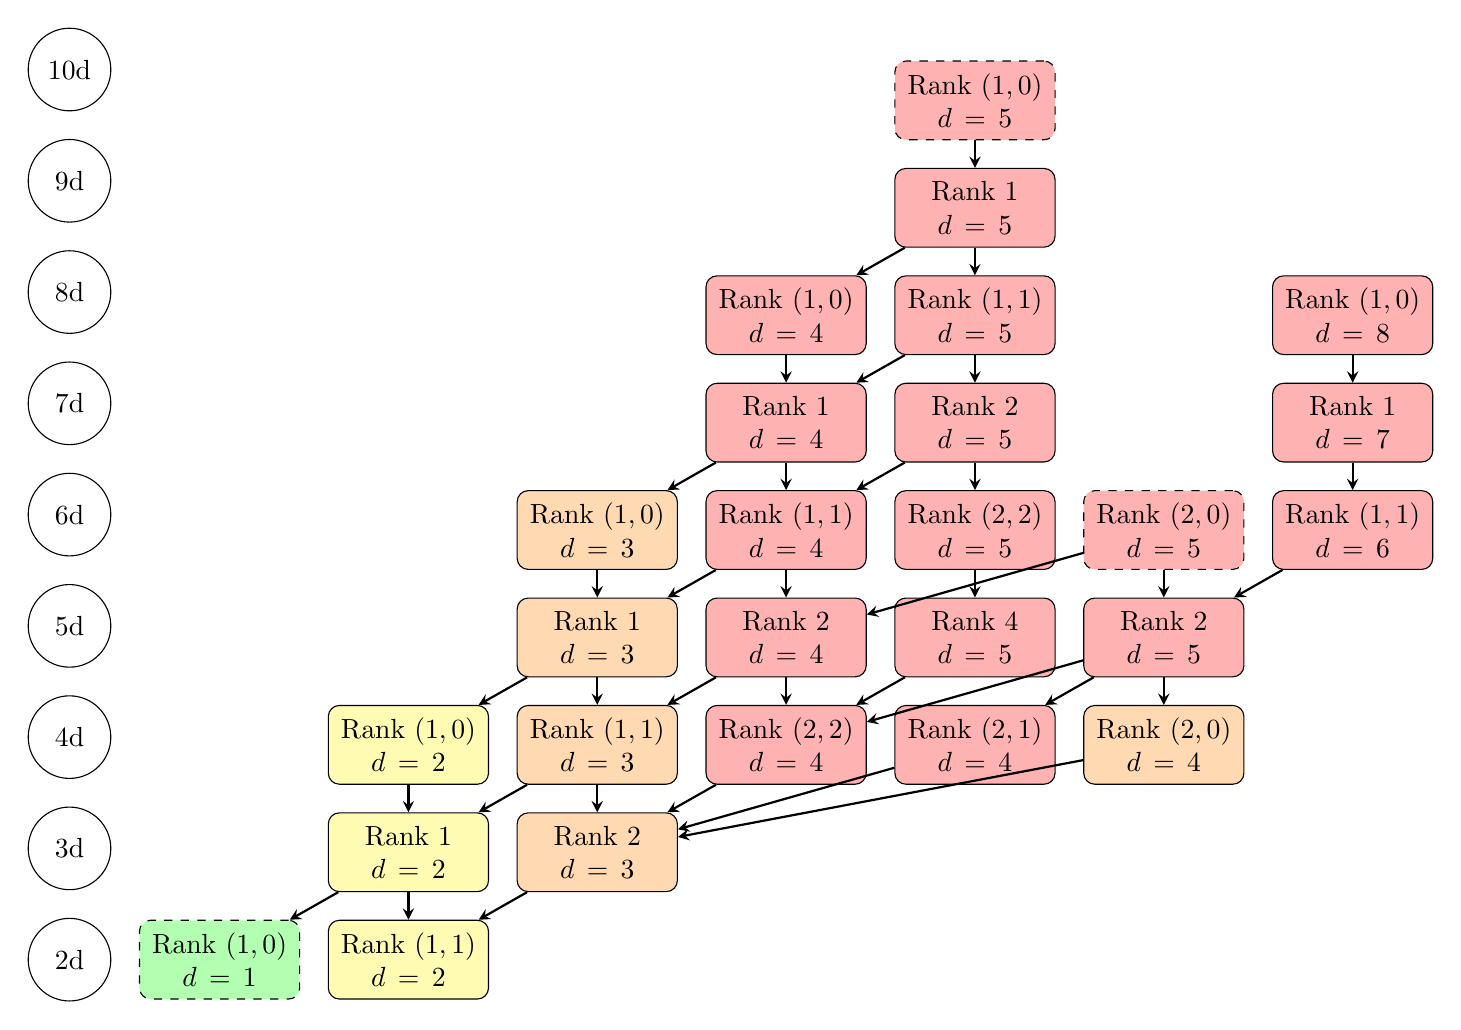
\begin{tikzpicture}[node distance=0.35cm and 0.35cm, text width=1.8cm]
\node (101) [s16chiral] {Rank $(1, 0)$ $d=5$};
\node (91) [s16, below=of 101] {Rank $1$ $d=5$};
\node (82) [s16, below=of 91] {Rank $(1, 1)$ $d=5$};
\node (81) [s16, left=of 82] {Rank $(1, 0)$ $d=4$};
\node (825) [right=of 82] {};
\node (83) [s16, right=of 825] {Rank $(1, 0)$ $d=8$};
\node (71) [s16, below=of 81] {Rank $1$ $d=4$};
\node (72) [s16, below=of 82] {Rank $2$ $d=5$};
\node (73) [s16, below=of 83] {Rank $1$ $d=7$};
\node (62) [s16, below=of 71] {Rank $(1, 1)$ $d=4$};
\node (61) [s8, left=of 62] {Rank $(1, 0)$ $d=3$};
\node (63) [s16, below=of 72] {Rank $(2, 2)$ $d=5$};
\node (64) [s16chiral, right=of 63] {Rank $(2, 0)$ $d=5$};
\node (65) [s16, below=of 73, right=of 64] {Rank $(1, 1)$ $d=6$};
\node (51) [s8, below=of 61] {Rank $1$ $d=3$};
\node (52) [s16, below=of 62] {Rank $2$ $d=4$};
\node (53) [s16, below=of 63] {Rank $4$ $d=5$};
\node (54) [s16, below=of 64] {Rank $2$ $d=5$};
\node (42) [s8, below=of 51] {Rank $(1, 1)$ $d=3$};
\node (41) [s4, left=of 42] {Rank $(1, 0)$ $d=2$};
\node (43) [s16, right=of 42] {Rank $(2, 2)$ $d=4$};
\node (44) [s16, right=of 43] {Rank $(2, 1)$ $d=4$};
\node (45) [s8, right=of 44] {Rank $(2, 0)$ $d=4$};
\node (31) [s4, below=of 41] {Rank $1$ $d=2$};
\node (32) [s8, below=of 42] {Rank $2$ $d=3$};
\node (22) [s4, below=of 31] {Rank $(1, 1)$ $d=2$};
\node (21) [s2chiral, left=of 22] {Rank $(1, 0)$ $d=1$};

\draw[arrow] (101) -- (91);
\draw[arrow] (91) -- (81);
\draw[arrow] (91) -- (82);
\draw[arrow] (81) -- (71);
\draw[arrow] (82) -- (71);
\draw[arrow] (82) -- (72);
\draw[arrow] (83) -- (73);
\draw[arrow] (71) -- (61);
\draw[arrow] (71) -- (62);
\draw[arrow] (72) -- (62);
\draw[arrow] (72) -- (63);
\draw[arrow] (73) -- (65);
\draw[arrow] (61) -- (51);
\draw[arrow] (62) -- (51);
\draw[arrow] (62) -- (52);
\draw[arrow] (63) -- (53);
\draw[arrow] (64) -- (52);
\draw[arrow] (64) -- (54);
\draw[arrow] (65) -- (54);
\draw[arrow] (51) -- (41);
\draw[arrow] (51) -- (42);
\draw[arrow] (52) -- (42);
\draw[arrow] (52) -- (43);
\draw[arrow] (53) -- (43);
\draw[arrow] (54) -- (43);
\draw[arrow] (54) -- (44);
\draw[arrow] (54) -- (45);
\draw[arrow] (41) -- (31);
\draw[arrow] (42) -- (31);
\draw[arrow] (42) -- (32);
\draw[arrow] (43) -- (32);
\draw[arrow] (44) -- (32);
\draw[arrow] (45) -- (32);
\draw[arrow] (31) -- (21);
\draw[arrow] (31) -- (22);
\draw[arrow] (32) -- (22);

\node (2d) [dimension, left=of 21] {2d};
\node (3d) [dimension, above=of 2d] {3d};
\node (4d) [dimension, above=of 3d] {4d};
\node (5d) [dimension, above=of 4d] {5d};
\node (6d) [dimension, above=of 5d] {6d};
\node (7d) [dimension, above=of 6d] {7d};
\node (8d) [dimension, above=of 7d] {8d};
\node (9d) [dimension, above=of 8d] {9d};
\node (10d) [dimension, above=of 9d] {10d};
\end{tikzpicture}
\caption{Orbits of square-zero supercharges.}
\label{fig:superchargeorbits}
\end{figure}
%\end{landscape}

% \subsection{Standard Equivalences Between Classical Field Theories}
% In this section, we will collect some standard lemmas that we'll use to simplify the descriptions of twisted supersymmetric field theories below.
% 
% \begin{lemma} \label{symplectomorphism_lemma}
% A linear symplectomorphism $F \colon \mc E^\bullet \to \mc E^\bullet$ induces an equivalence of theories between $(\mc E^\bullet, Q, \omega, I)$ and $(\mc E^\bullet, F^*Q, \omega, F^*I)$.
% \end{lemma}
% 
% \brian{I may be optimistic, but shouldn't the lemmas below all follow from the fact that the category we are working with is a Grothendieck abelian category? In any case, I do like that we've stated them clearly.} \chris{I'm not sure what you have in mind (for instance I'm not sure why you would need the Grothendieck condition there), but I think the lemmas below should be formally immediate in this dg category of differentiable cochain complexes setting (like the first one follows in any context where you have an exact sequence $0 \to A \to B \to C \to 0$ and the fact that if $C$ is equivalent to 0 then $A \to B$ is an equivalence, or the same with $A$ and $B \to C$.)}
% 
% \begin{lemma} \label{inclusion_and_projection_lemma}
% Let $(\mc E^\bullet, Q)$ be a cochain complex, and let $(\mc C^\bullet, Q')$ be a contractible cochain complex.
% \begin{enumerate}
%  \item Let $F \colon \mc C^\bullet \to \mc E^\bullet$ be a degree 1 map making $(\mc C^\bullet \overset F\to \mc E^\bullet)$ into a cochain complex.  Then the canonical inclusion $\mc E^\bullet \to (\mc C^\bullet \overset F\to \mc E^\bullet)$ is a quasi-isomorphism.
%  \item Let $F' \colon \mc E^\bullet \to \mc C^\bullet$ be a degree 1 map making $(\mc E^\bullet \overset {F'}\to \mc C^\bullet)$ into a cochain complex.  Then the canonical projection $(\mc E^\bullet \overset {F'}\to \mc C^\bullet) \to \mc E^\bullet$ is a quasi-isomorphism.
% \end{enumerate}
% \end{lemma}
% 
% \begin{lemma} \label{symplectic_composite_lemma}
% Let $(\mc E^\bullet,Q)$ be a cochain complex, let $(\mc C_1^\bullet, Q_1)$ and $(\mc C_2^\bullet, Q_2)$ be contractible cochain complexes, and let $\mc C_1^\bullet \overset{F_1}\to \mc E^\bullet \overset{F_2}\to \mc C_2^\bullet$ be a pair of degree 1 maps so that the differential $Q + Q_1 + Q_2 + F_1 + F_2$ on the total complex squares to 0.  Suppose the graded vector space $\mc E^\bullet \oplus \mc C_1^\bullet \oplus C_2^\bullet$ is equipped with a $-1$-shifted symplectic structure so that $\mc C_1^\bullet \oplus \mc C_2^\bullet$ is a symplectic subspace.  Then the cochain map 
% \begin{equation}
% \label{symp_composite_eqn}\mc E^\bullet \to (\mc C_1^\bullet \overset{F_1}\to \mc E^\bullet \overset{F_2}\to \mc C_2^\bullet)
% \end{equation}
% obtained as the composite of the projection from Lemma \ref{inclusion_and_projection_lemma} (2) with a quasi-inverse to the inclusion from Lemma \ref{inclusion_and_projection_lemma} (1) is a symplectomorphism.
% \end{lemma}
% 
% \begin{lemma} \label{interaction_pullback_lemma}
% In the set-up of Lemma \ref{symplectic_composite_lemma}, suppose we're given an interaction $I$ on the graded vector space $\mc E^\bullet \oplus \mc C_1^\bullet \oplus \mc C_2^\bullet$, which pulls back to $I'$ under the inclusion of $\mc E^\bullet$.  Suppose that all monomial summands of the interaction $I$ which depend on fields in $\mc C_2^\bullet$ also depend on fields in $\mc C_1^\bullet$. Then the map \ref{symp_composite_eqn} is compatible with the interactions $I$ and $I'$
% \end{lemma}
% 
% \begin{proof}
% We defined a quasi-isomorphism of cochain complexes in Lemma \ref{symplectic_composite_lemma} to be the composite $F$ of the inclusion $i$ of $\mc E^\bullet \oplus \mc C_2^\bullet$ with a quasi-inverse to the projection onto $\mc E^\bullet$: this composite map is a twisted inclusion $\mc E^\bullet \to \mc E^\bullet \oplus \mc C_1^\bullet \oplus \mc C_2^\bullet$ of the form $F \colon \phi \mapsto (\phi, 0, f(\phi))$ for some linear map $f$.  Because, by the hypothesis, all monomial summands of $I$ involving fields in $\mc C_2^\bullet$ also include fields in $\mc C_1^\bullet$, the pullback of $I$ under the map $F$ coincides with the pullback of $I$ under the inclusion map $\phi \mapsto (\phi, 0, 0)$ as required.
% \end{proof}
% 
% \subsection{A-Type Twists} \label{A_twist_section}
% \chris{...}
% 
% \subsection{Dimension 10}
% We'll begin our discussing of twists of super Yang-Mills theory by studying the twist of 10-dimensional $\mc N=(1,0)$ super Yang-Mills theory, with the supersymmetry action we analyzed in Section \ref{sect:gaugemultipletSUSY}.  In the 10d $\mc N=(1,0)$ supersymmetry algebra there is a unique $\Spin(10)$ orbit of non-trivial square-zero supercharges given by the locus of pure spinors.  These square-zero supercharges are holomorphic.
% 
% Fix a non-trivial pure spinor $Q$, or equivalently, fix a Calabi-Yau structure on $\RR^{10}$.  The stabilizer of $Q$ in $\Spin(10)$ is isomorphic to $\SU(5)$.  Let us first, therefore, decompose the component fields of 10d super Yang-Mills theory into sections of the associated bundles to irreducible representations of $\SU(5)$.  The BRST fields split as follows:
% \begin{align*}
% c &\mapsto c \in \Omega^0(\CC^5; \gg) \\
% A &\mapsto A_{0, 1} + A_{1, 0} \in \Omega^{0,1}(\CC^5; \gg) \oplus \Omega^{1,0}(\CC^5; \gg)\\
% \lambda &\mapsto \chi + \psi + B \in \Omega^0(\CC^5; \gg) \oplus \Omega^{1,0}(\CC^5; \gg) \oplus \Omega^{0,2}(\CC^5; \gg). 
% \end{align*}
% 
% In terms of these component fields, the BV action can be written in the following way.  We will split the BV action up into the BRST action and the antifield action.
% \begin{align*}
% S_{\mr{BRST}} &= \int \d^5z \left(\Lambda^2 \langle F_{0,2} \wedge F_{2,0}\rangle + \frac 12 |\Lambda F_{1,1}|^2 + \Lambda( \chi \wedge (\ol \dd_{A_{0,1}} \psi))  + \Lambda^2(B \wedge (\dd_{A_{1,0}} \psi))\right) \Omega + (B \wedge \ol \dd_{A_{0,1}} B) \\
% S_{\mr{anti}} &= \int \d^5z \langle \dd_{A_{1,0}}c, A_{1,0}^\vee \rangle +  \langle \ol \dd_{A_{0,1}}c, A_{0,1}^\vee \rangle + \langle [c,c], c^\vee \rangle + \langle [\chi,c], \chi^\vee \rangle + \langle [\psi,c], \psi^\vee \rangle + \langle [B,c], B^\vee \rangle,
% \end{align*}
% where $F_{i,j}$ is the $(i,j)$-form component of the curvature of the gauge field $A_{0, 1} + A_{1, 0}$, and $\Omega$ is the Calabi-Yau $(0,5)$-form.  Similarly, we can write explicitly the $L_\infty$ interaction functional associated to the action of the square 0 supercharge $Q$.  It has a quadratic and a cubic component given by
% \begin{align*}
% I^{(1)} &= \int \langle A_{1,0}^\vee, \psi \rangle + \langle \chi^\vee \Lambda F_{1,1} \rangle + \langle B^\vee, F_{0,2} \rangle \\
% I^{(2)} &= \frac 12 \int \d^5z \Omega |\chi^\vee|^2.
% \end{align*}
% The twisted action functional is obtained by adding these terms to the original BV action functional.
% 
% We can now calculate the 10d holomorphic twist.  This calculation is originally due to Baulieu \cite{Baulieu}.
% 
% \begin{theorem}\label{10d_twist_thm}
% The holomorphic twist of 10d super Yang-Mills theory on a Calabi-Yau 5-fold $X_5$ is equivalent to holomorphic Chern-Simons theory on $X_5$.
% \end{theorem}
% 
% \begin{remark}
% From the point of view of supersymmetry, the twisted theory is only $\ZZ/2\ZZ$-graded, because the R-symmetry group is trivial, so there is no possible R-charge with which to regrade the twisted theory to make it $\ZZ$-graded.  
% This is of course compatible with our conventions for holomorphic Chern-Simons: holomorphic Chern-Simons (with values in an ordinary Lie algebra) on an odd dimensional Calabi-Yau only defines a $\ZZ/2$-graded theory (unless $d=3$, where this can be lifted to a $\ZZ$-grading). 
% As a consequence, the twisted BV-BRST complex only has an odd symplectic pairing, not a $(-1)$-symplectic pairing.
% \end{remark}
% 
% \begin{proof}
% We'll prove this equivalence by first describing an equivalence of the underlying classical theories, as the composite of several maps, then showing that this equivalence is compatible with the two interaction functionals, and therefore defines a morphism of classical field theories, and finally observing that by Lemma \ref{free_int_ss_lemma} this morphism is automatically an equivalence.
% 
% \begin{enumerate}
%  \item The first part of our equivalence of classical field theories will be a simple change of variables.  Let $\chi'^\vee = \chi^\vee + \Lambda F_{1,1}$, and dually let $\chi' = \chi + \Lambda F_{1,1}^\vee$.  In terms of $\chi'$, the quadratic part of the twisted action functional becomes
%  \begin{align*}
%   S^Q &= \int \d^5z \left(\Lambda^2 \langle \ol \dd A_{0,1} \wedge \dd A_{1,0} \rangle + \frac 12 |\chi'^\vee|^2 + \Lambda( \chi' \wedge (\ol \dd \psi)) - \Lambda^2(\dd A_{0,1} \wedge \ol \dd \psi) + \Lambda^2(B \wedge (\dd \psi))\right) \Omega + (B \wedge \ol \dd B) \\
%   &\quad + \langle \dd c, A_{1,0}^\vee \rangle +  \langle \ol \dd c, A_{0,1}^\vee \rangle + \langle A_{1,0}^\vee, \psi \rangle + \langle B^\vee, \ol \dd A_{0,1} \rangle.
%  \end{align*}
%  The classical BV complex associated to the theory after performing this change of variables is quasi-isomorphic to the classical BV complex of the original theory according to Lemma \ref{symplectomorphism_lemma}.  However, after performing the change of variables, the classical BV complex takes the form $(\Omega^0(\CC^5; \gg)_{\chi'^\vee} \overset \id \to \Pi\Omega^0(\CC^5; \gg)_{\chi'}) \to \mc E^\bullet$, where $\mc E^\bullet$ is the part of the BV complex generated by all fields other than $\chi'$ and $\chi'^\vee$, and where the map into $\mc E^\bullet$ is given by the map $\ol \dd$ from $\chi$ to $\psi^\vee$.  Therefore the inclusion of the complex $\mc E^\bullet$ is a quasi-isomorphism by Lemma \ref{inclusion_and_projection_lemma}.  We think of this as ``integrating out'' the field $\chi'$ and its antifield.
%  
%  \item We'll now use a similar trick to integrate out the fields $\psi, A_{1,0}$ and their antifields.  We've argued in step 1 that the free part of the $Q$-twisted theory is equivalent to the theory with action functional 
%  \[  S^Q = \int \d^5z \left(\Lambda^2 \langle \ol \dd A_{0,1} \wedge \dd A_{1,0} \rangle + \Lambda^2(B \wedge (\dd \psi))\right) \Omega + (B \wedge \ol \dd B) + \langle \dd c, A_{1,0}^\vee \rangle +  \langle \ol \dd c, A_{0,1}^\vee \rangle + \langle A_{1,0}^\vee, \psi \rangle + \langle B^\vee, \ol \dd A_{0,1} \rangle.\]
%  We'll begin, as in step 1, by performing a linear change of variables, setting $A'_{1,0} = A_{1,0} - \ol{A_{0,1}}$, and performing the dual change of variables on the antifields.  This change of variables has the effect of eliminating the term $\langle \dd c, A_{1,0}^\vee \rangle$ from the quadratic part of the action. \chris{This isn't quite right I think.  We need to kill that term, however, for the below argument to work.  Can we fix it?}
%  
%  Observe that the classical BV complex associated to this action functional can now be written in the following form:
%  \[\xymatrix{
%  &&\Omega^{1,0}(\CC^5;\gg)_\psi \ar[dl] \ar[dr] \ar[r] &\Omega^{1,0}(\CC^5;\gg)_{{A'}_{1,0}} \ar[dr]\\
%  \Omega^0(\CC^5;\gg)_c \ar[r] &\Omega^{0,1}(\CC^5;\gg)_{A_{0,1}}  \ar[dl] \ar[r] &\Omega^{0,2}(\CC^5;\gg)_{B} \ar[dl]\ar[r] &\Omega^{0,3}(\CC^5;\gg)_{B^\vee} \ar[r] &\Omega^{0,4}(\CC^5;\gg)_{A_{0,1}^\vee} \ar[dlll] \ar[r] &\Omega^{0,5}(\CC^5;\gg)_{c^\vee} \\
%  \Omega^{4,0}(\CC^5;\gg)_{{A'}_{1,0}^\vee} \ar[r]   &\Omega^{4,0}(\CC^5;\gg)_{\psi^\vee},
%  }\]
%  where the first and third rows are dual under the symplectic pairing.  This is exactly in the form required to apply Lemma \ref{symplectic_composite_lemma}, so applying that result tells us that the underlying free theory of the twisted 10d super Yang Mills theory is equivalent to the middle row alone, i.e. the Dolbeault complex, which is exactly the free part of holomorphic Chern-Simons theory on $\CC^5$.
%  
%  \item Now, let's understand how the interaction functional behaves under this equivalence of classical field theories.  The morphism from step 1 is just given by an inclusion, so the interaction on twisted 10d Yang-Mills theory is compatible with the interaction evaluated at $\chi'=\chi'^\vee=0$.  In order to make the same observation for the fields $\psi$ and $A_{1,0}$, we'll use Lemma \ref{interaction_pullback_lemma}, which we can apply using the observation that the antifields $A_{1,0}^\vee$ and $\psi^\vee$ only appear in the action together with the corresponding fields.  Take our original action functional after the change of variables from step 1, and set the fields $\chi, \psi, A_{1,0}$ and their antifields to zero (i.e, in the notation of Lemma \ref{interaction_pullback_lemma}, restrict the interaction to the complex $\mc E^\bullet$).  The resulting interaction is 
%  \[
%   I^Q = \int \d^5z (B \wedge [A_{0,1} \wedge B]) + \langle B^\vee, [A_{0,1} \wedge A_{0,1}] \rangle + \langle [c,c], c^\vee \rangle + \langle [A_{0,1}, c], A_{0,1}^\vee \rangle + \langle [B,c], B^\vee \rangle,
%  \]
%  which is, indeed, the interaction functional for holomorphic Chern-Simons theory.  The composite of the morphisms in steps 1 and 2 therefore defines a morphism of classical field theories from holomorphic Chern-Simons theory to twisted 10d super Yang-Mills theory.
%  
%  \item To conclude the proof, we only need to apply Lemma \ref{free_int_ss_lemma}.  The morphism of classical field theories that we've constructed induces an equivalence of the $E_1$ pages of the free-to-interacting spectral sequences associated to holomorphically twisted 10d super Yang-Mills theory and holomorphic Chern-Simons theory.  Because the spectral sequences are convergent, there is likewise an equivalence of the $E_\infty$ pages, i.e. an equivalence of classical field theories.
% \end{enumerate}
% \end{proof}
% 
% The above argument can be applied identically on a general Calabi-Yau 5-fold $X$.
% \brian{How do we place 10d YM on an arbitrary 5-fold? 
% Are you using something about sugra?
% } \chris{Not an arbitrary 5-fold, but just Calabi-Yau.  I'm not thinking of using sugra.  Instead I want to say that a Calabi-Yau 5-fold has a principal $\SU(5)$ frame bundle.  Take the fields to be sections of the associated vector bundles under the appropriate representations, then use the same action functional: the Lagrangian density is $\SU(5)$ invariant and so will define a density on the 5-fold.}
% 
% 
% \subsection{Dimension 9}
% The 9-dimensional $\mc N=1$ super Yang-Mills theory is obtained by dimensional reduction of $\mc N=1$ super Yang-Mills from $\RR^{10}$ to $\RR^9$.  It has BRST fields given by a ghost, a 9d gauge field $A$, a $\gg$-valued scalar field $\phi$, and a Dirac spinor field $\lambda$.
% 
% There is a single non-zero equivalence class of square zero supercharges in 9 dimensions. Such supercharges are minimal (i.e. have 5d image).  They are stabilized by $\SU(4)$.  Like in 10 dimensions, the R-symmetry group is trivial, and so the twisted theory by such a supercharge is only $\ZZ/2\ZZ$-graded.
% 
% Let's describe the twist of 9-dimensional $\mc N=1$ theory with respect to such a supercharge.  The relevant fields for this calculation are those component fields which survived the 10d holomorphic twist of Theorem \ref{10d_twist_thm}.  These fields, in the BRST formalism, decompose, under the action of $\SU(4)$ into the following component fields:
% \begin{align*}
% B^{10} &= B + A \wedge \d \ol z^5 \in (\Omega^{0,2}(\CC^4; \gg) \oplus \Omega^{0,1}(\CC^4; \gg)) \otimes \Omega^0(\RR_{x^9}) \\
% A^{10}_{0,1} &= A' + \phi \d \ol z^5 \in (\Omega^{0,1}(\CC^4; \gg) \oplus \Omega^0(\CC^4; \gg)) \otimes \Omega^0(\RR_{x^9})
% \end{align*}
% along with the ghost $c$.  We'll describe the twisted action functional using dimensional reduction.
% 
% \brian{Where is the one-form in the $\RR$-direction? Are we identifying that with $\phi$?}
% 
% \begin{theorem} \label{9d_twist_thm}
% The minimal twist of 9d super Yang-Mills theory on the product of a Calabi-Yau 4-fold $X_4$ and an oriented 1-manifold $L = \RR$ or $S^1$ is equivalent to mixed Chern-Simons theory on $X_4 \times L_\mr{dR}$.
% \end{theorem}
% 
% \begin{proof}
% Let's apply Lemma \ref{commuting_twist_and_reduction_lemma} -- the fact that twisting commutes with dimensional reduction.  Choose a representative element $Q$ in the equivalence class of square-zero supercharges which also squares to zero in the 10d $\mc N=(1,0)$ supersymmetry algebra.  According to Lemma \ref{commuting_twist_and_reduction_lemma}, the twist of 9d $\mc N=1$ super Yang-Mills theory by the supercharge $Q$ is equivalent to the dimensional reduction of holomorphic Chern-Simons theory on $X_4 \times C$, where $C = L \times \RR$ is either the curve $\CC$ if $L = \RR$, or $\CC^\times$ if $L = S^1$. 
% 
% As such, it's sufficient to observe that mixed Chern-Simons theorem on $X_4 \times L_{\mr{dR}}$ is a dimensional reduction of holomorphic Chern-Simons theory on $X_4 \times C$, which follows by applying Lemma \ref{CS_diml_red_prop}.
% \end{proof}
% 
% \begin{remark}
% One can, alternatively, prove this theorem using exactly the same methods as Theorem \ref{10d_twist_thm}; the steps that one needs to follow are identical.
% \end{remark}

\section{Dimension 8}
\vspace{-10pt}
\paragraph{Fields:} 
The 8-dimensional $\mc N=1$ super Yang-Mills theory is obtained by dimensional reduction of $\mc N=1$ super Yang-Mills from $\RR^{10}$ to $\RR^8$.  It has BRST fields given by a ghost $c$ along with the following.
\begin{itemize}
 \item Bosons: an 8d gauge field $A$ in $\Omega^1(\RR^8; \gg)$, and a pair of $\gg$-valued scalar fields $\phi_1$ and $\wt \phi_1$ in $\Omega^0(\RR^8; \gg)$.
 \item Fermions: a Dirac spinor field $\lambda = (\lambda_+, \lambda_-) \in \Omega^0(\RR^8; \gg \otimes(S_+ \oplus S_-))$.
\end{itemize}

We will see shortly that in the 8d $\mc N=1$ supersymmetry algebra there are holomorphic square-zero supercharges stabilized by the group $\SU(4)$, and topological square-zero supercharges stabilized by $\spin(7)$.  If we want to stabilize the full one-parameter family describing the degeneration, we have to decompose our fields according to the action of the intersection $\SU(4) \cap \spin(7) \iso \SU(3)$ \chris{check this claim: can we see it in terms of the Dynkin diagrams?}.  So, let's begin by establishing notation for the BRST fields of maximal super Yang-Mills after reduction to representations of various subgroups of $\SO(10)$.  We can write this schematically in the following way.

First, let us consider the reduction of the 10d spinor $\lambda$.  We have already described the decomposition of the spinor representation into irreducible summands for the group $\SU(5)$: it decomposes into a sum $B_{0,2} + \psi_{1,0} + \chi$ of a $(0,2)$-form, a $(1,0)$-form, and a scalar (all valued in the Lie algebra $\gg$).  We have also already described its decomposition into irreducible summands for the group $\mr O(8)$: it splits into a positive and a negative Weyl spinor, $\lambda^+ + \lambda^-$.  Let us continue to decompose these fields into smaller subgroups.  We indicate this schematically as follows (Figure \ref{fig:8dfermiondecomp}).
\begin{figure}[!h]
\[
\xymatrix{
&\lambda \ar[dl]_{\to\,  \mr{O}(8)} \ar[dr]^{\to\,  \SU(5)} &\\
\lambda^+, \lambda^- \ar[dr]_{\to\,  \SU(4)} \ar[d]_{\to\,  \Spin(7)} &&B_{0,2}, \psi_{1,0}, \chi \ar[dl]^{\to\,  \SU(4)} \\
(A_7^+, \wt \chi^+), \lambda^- \ar[dr] &(B_{0,2}^+, \psi_{0,1}^-), (\psi_{1,0}^+, \wt \chi^-), \chi^- \ar[d]_{\to\,  \SU(3)} &\\
 &((\psi_{1,0}^+, \psi_{0,1}^+), (\psi_{0,1}^-, \chi^-)), ((\psi_{1,0}^-, \wt \chi^-), \wt \chi^+), \chi^+. &
}\]
\caption{Decomposition of the 10d fermionic field $\lambda$ upon restriction to subgroups of $\mr O(10)$.}
\label{fig:8dfermiondecomp}
\end{figure}
In this diagram, the superscript $\pm$ indicates whether each component field arose as a summand of $\lambda^+$ or $\lambda^-$.  The $\chi^\pm$ and $\wt \chi^\pm$ are $\gg$-valued scalars, and the fields $A_7^\pm$ are $\gg$-valued elements of the vector representation of $\spin(7)$.  Finally, we have used parentheses to indicate how the fields decompose under the restriction from $\SU(n)$ to $\SU(n-1)$.

We can do the same for the decomposition of the 10d gauge field $A$.  Again, we indicate this schematically as follows (Figure \ref{fig:8dbosondecomp}).
\begin{figure}[!h]
\[\xymatrix{
&A \ar[dl]_{\to\,  \mr{O}(8)} \ar[dr]^{\to\,  \SU(5)} & \\
A,\phi_1, \wt \phi_1 \ar[dr]_{\to\,  \SU(4)} \ar[d]_{\to\,  \Spin(7)} &&A_{0,1}, A_{1,0} \ar[dl]^{\to\,  \SU(4)} \\
\lambda_7, \phi_1, \wt \phi_1 \ar[dr] &A_{0,1},A_{1,0},\phi_1, \wt \phi_1 \ar[d]_{\to\,  \SU(3)} & \\
&(A_{0,1}, \phi_2) ,(A_{1,0}, \wt \phi_2) \phi_1, \wt \phi_1.&
}
\]
\caption{Decomposition of the 10d bosonic field $A$ upon restriction to subgroups of $\mr O(10)$.}
\label{fig:8dbosondecomp}
\end{figure}
Now $\phi_i$ and $\wt \phi_i$ denote $\gg$-valued scalar fields, and $\lambda_7$ denotes a field valued in the spinor representation of $\Spin(7)$.

\vspace{-10pt}
\paragraph{Supersymmetry action:} 
Using the decomposition of the fields described above, we can describe the supersymmetric interaction terms $I^{(1)}$ and $I^{(2)}$ after reduction from 10d to 8d, with respect to various subgroups of $\mr O(8)$.  We begin by considering $\mr O(8)$ itself.

\begin{prop} \label{O8_decomposition_of_susy_prop}
After reduction to $\mr O(8)$, the interaction terms $I^{(1)}$ and $I^{(2)}$ become
\begin{align*}
I^{(1)}(Q^+) &= \langle A^\vee, \Gamma(Q^+, \lambda^-)\rangle + \langle \phi_1,^\vee (Q^+,\lambda^+)\rangle + \langle \lambda^{+\vee}, \sd F_A Q_+ \rangle + \langle \lambda^{-\vee}, \rho(\dd \phi_1)Q_+ \rangle\\
I^{(2)}(Q^+, Q^+) &= (\lambda^{+\vee}, \lambda^{+\vee})(Q^+,Q^+) + (\lambda^{+\vee},Q^+)^2 + \langle c^\vee, \phi_1\rangle(Q_+,Q_+)
\end{align*}
if $Q^+$ is an element of $S_+$, and
\begin{align*}
I^{(1)}(Q^-) &= \langle A^\vee, \Gamma(Q^-, \lambda^+)\rangle + \langle \wt \phi_1^\vee, (Q^-,\lambda^-)\rangle+ \langle \lambda^{-\vee}, \sd F_A Q_- \rangle + \langle \lambda^{+\vee}, \rho(\dd \wt \phi_1)Q_- \rangle\\
I^{(2)}(Q^-, Q^-) &= (\lambda^{-\vee}, \lambda^{-\vee})(Q^-,Q^-) + (\lambda^{-\vee},Q^-)^2 + \langle c^\vee, \wt \phi_1\rangle(Q_-,Q_-)
\end{align*}
if $Q^-$ is an element of $S_-$.
\end{prop}

\begin{proof}
There are two ingredients in this calculation: we have to decompose our fields as representations of $\mr O(8)$, and simultaneously we have to write the 10d $\Gamma(-,-)$ pairing in terms of the corresponding pairing for 8d spinors, upon dimensional reduction. \chris{Pavel gave this argument, in terms of light-cone coordinates.}
\end{proof}

\begin{remark}
A Weyl spinor $Q_\pm$ corresponds to a holomorphic twist (i.e. comes from a 10d square zero supercharge) exactly when $(Q_\pm,Q_\pm)=0$ -- in that case many of the terms in the interaction above will vanish.
\end{remark}

\vspace{-10pt}
\paragraph{Twisting data:}
In 8 dimensions, there are 3 classes of inequivalent non-zero supercharges by which we can twist.
\begin{enumerate}
 \item Pure spinors, for which either $\lambda_+ = 0$ or $\lambda_- = 0$.  These supercharges are holomorphic.  They are stabilized by $\SU(4)$.  Twists by pure spinors can be made $\ZZ$-graded using a maximal torus in the R-symmetry group $\GL(1)$.
 \item Impure square-zero spinors with $\lambda_+ = 0$ or $\lambda_- = 0$.  These supercharges are topological.  They are stabilized by $\Spin(7) \sub \SO(8)$.  Again, twists by such supercharges can be made $\ZZ$-graded.
 \item Square-zero spinors where both $\lambda_+$ and $\lambda_-$ are non-zero.  Such supercharges have a 5-dimensional image in $\CC^8$.  Twists by such supercharges are still only $\ZZ/2\ZZ$-graded.
\end{enumerate}

When we dimensionally reduce the minimally twisted 10- or 9-dimensional super Yang-Mills theories to 8 dimensions we obtain either the twist by a supercharge of type 1, or of type 3, depending on whether we reduce along an invariant direction or a non-invariant direction, as indicated on the ``8d'' row of Figure \ref{fig:superchargeorbits}.  The topological twist (type 2 in the list above) appears in the right-most column of the figure, and is not obtained by dimensional reduction from higher dimensions.

Square-zero supercharges in the 10d $\mc N=(1,0)$ supersymmetry algebra correspond to holomorphic supercharges in the 8d $\mc N=1$ supersymmetry algebra.  As such, we can calculate the holomorphic twist of 8d $\mc N=1$ super Yang-Mills by dimensionally reducing the holomorphic twist of 10d $\mc N=(1,0)$ super Yang-Mills along a copy of $\CC$.  This theory can, unlike its 10- and 9-dimensional analogues, be made canonically $\ZZ$-graded.

On the other hand, the topological twist -- the twist by an impure Weyl spinor -- of 8d $\mc N=1$ super Yang-Mills theory does not arise by dimensionally reducing a twisted theory in 9 dimensions.  This will be our first example of an A-type twist, as we discussed in Section \ref{A_twist_section} \chris{to add}: we will understand it as a one parameter family of supercharges, degenerating at zero to the holomorphic twist -- the twist by a pure Weyl spinor.

Let us now consider the further reductions to $\SU(4)$, to $\spin(7)$, and to their intersection $\SU(3)$.  We will use the form of the supersymmetric interaction term above to prove the following.

\begin{theorem} \label{8d_holo_twist_thm}
The holomorphic twist of 8d $\mc N=1$ super Yang-Mills theory on a Calabi-Yau 4-fold $X_4$ is equivalent to holomorphic BF theory on $X_4$. If $X_4$ splits into a product $X_3 \times S$ of a Calabi-Yau 3-fold and a flat surface, then this twist degenerates to a one-parameter family of topological twists of the form $\map(X_3 \times S, B\gg)_{\mr{Hod}}$.
\end{theorem}

\begin{proof}
We begin by describing the twist by a holomorphic supercharge $Q_+$, on a Calabi-Yau 4-fold $X_4$.  We can do this by by applying Lemma \ref{CS_to_BF_diml_red_prop} to the minimal twist of 9d super Yang-Mills theory.  More explicitly, the minimal twist of 9d super Yang-Mills theory on $X_4 \times L$ is modelled by mixed Chern-Simons theory on $X_4 \times L_\mr{dR}$. Lemma \ref{CS_to_BF_diml_red_prop} says that if we reduce this mixed Chern-Simons theory in the $L$-direction, we obtain a holomorphic BF theory described by $\map(X_4, T[1]B\gg)$

Note that, unlike in 9d, this theory can be made $\ZZ$-graded, rather than just $\ZZ/2\ZZ$-graded.  To do so, we consider the action of the 8d R-symmetry group $\CC^\times$, where $S_+$ has weight $+1$ and $S_-$ has weight $-1$, so in particular the holomorphic supercharge $Q_+$ has weight 1.  We've chosen notation for our component fields that makes it easy to read off the R-symmetry weight of each field: fermions with superscript $+$ have weight $+1$, fermions with superscript $-$ have weight $-1$, the bosonic scalars $\phi_1$ and $\wt \phi_1$ have weight -$2$, and the other bosons have weight 0.  With respect to this $\ZZ$-grading, the classical BV complex, as an $\SU(4)$-module, has the form
\[\xymatrix{&\Omega^0(X_4; \gg)_c \ar[r] &\Omega^{0,1}(X_4; \gg)_{A_{0,1}} \ar[r] &\Omega^{0,2}(X_4; \gg)_{B^+_{0,2}} \ar[r] &\Omega^{0,3}(X_4; \gg)_{\psi_{0,1}^{-\vee}} \ar[r] &\Omega^{0,4}(X_4; \gg)_{\phi_1^\vee} \\
\Omega^0(X_4; \gg)_{\phi_1} \ar[r] &\Omega^{0,1}(X_4; \gg)_{\psi_{0,1}^{-}} \ar[r] &\Omega^{0,2}(X_4; \gg)_{B^{+\vee}_{0,2}} \ar[r] &\Omega^{0,3}(X_4; \gg)_{A_{0,1}^\vee} \ar[r] &\Omega^{0,4}(X_4; \gg)_{c^\vee}&
}\]
placed in cohomological degrees $-2, \ldots, 3$.

Now, suppose $X_4$ splits into a product of the form $X_3 \times S$.  If we restrict to $\SU(3)$ representations, our classical BV complex becomes

\resizebox{1.05\textwidth}{!}{$\xymatrix@C-20pt{&\Omega^0(X_3 \times S; \gg)_c \ar[r] \ar[rd] &\Omega^{0,1}(X_3 \times S; \gg)_{A_{0,1}} \ar[r] \ar[rd] &\Omega^{0,2}(X_3 \times S; \gg)_{\psi^+_{1,0}} \ar[r]  &\Omega^{0,3}(X_3 \times S; \gg)_{\chi^{-\vee}} \ar[rd] & \\
&&\Omega^0(X_3 \times S; \gg\omega)_{\phi_2} \ar[r] &\Omega^{0,1}(X_3 \times S; \gg\omega)_{\psi^{+}_{0,1}} \ar[r] &\Omega^{0,2}(X_3 \times S; \gg\omega)_{\psi^{-\vee}_{0,1}} \ar[r] &\Omega^{0,3}(X_3 \times S; \gg\omega)_{\phi_{1}^{\vee}} \\
\Omega^0(X_3 \times S; \gg)_{\phi_1} \ar[r] \ar[rd] &\Omega^{0,1}(X_3 \times S; \gg)_{\psi_{0,1}^{-}} \ar[r] \ar[rd] &\Omega^{0,2}(X_3 \times S; \gg)_{\psi^{+\vee}_{0,1}} \ar[r] \ar[rd] &\Omega^{0,3}(X_3 \times S; \gg)_{\phi_{2}^\vee} \ar[rd]&& \\
&\Omega^0(X_3 \times S; \gg\omega)_{\phi_1} \ar[r] &\Omega^{0,1}(X_3 \times S; \gg\omega)_{\psi_{1,0}^{+\vee}} \ar[r] &\Omega^{0,2}(X_3 \times S; \gg\omega)_{A_{0,1}^\vee} \ar[r] &\Omega^{0,3}(X_3 \times S; \gg\omega)_{c^\vee}&}
$}
where Dolbeault forms here refer to forms on $X_3$, and $\omega$ denotes the volume form on $S$.

Let $Q = Q^+ + tQ'$ be a generically topological 1-parameter family of supercharges in $S_+$, where $Q'$ is an impure spinor stabilized by $\spin(7)$.  The supercharges $Q_+$ and $Q'$ automatically commute, so to complete the proof it remains for us to compute the action of the further supercharge $Q'$ on the classical BV complex above.  To do so we will use the description of the supersymmetry action from Proposition \ref{O8_decomposition_of_susy_prop}.  So, we'll first observe that several summands of $I^{(1)}(Q')$ and $I^{(2)}(Q')$ are forced to vanish.  In $I^{(1)}(Q')$, the term pairing $\lambda_+^\vee$ and $A$ cannot be $\spin(7)$-invariant, so must vanish.  The same applies to the term pairing $\lambda_-^\vee$ and $\phi_1$. We are left with, in terms of $\Spin(7)$-fields,
\begin{align*}
I^{(1)}(tQ') &= t\langle\lambda_7^\vee, \lambda^-\rangle + t\langle \phi_1^\vee, \chi^+\rangle \\
I^{(2)}(tQ', tQ') &= t^2\langle c^\vee, \phi_1\rangle + t^2 (A_7^{+\vee} , A_7^{+\vee}),
\end{align*}
where we pair $A_7^{+\vee}$ with itself using the restriction of the scalar pairing on $S_+$ to the 7d vector representation \chris{can probably be phrased in terms of the $\spin(7)$-structure somehow}.  Restricting to representations of $\SU(3)$, this takes the form
\begin{align*}
I^{(1)}(tQ') &= t\langle A_{0,1}^\vee, \psi_{0,1}^-\rangle + t\langle \phi_1^\vee, \chi^+\rangle \\
I^{(2)}(tQ', tQ') &= t^2\langle c^\vee, \phi_1\rangle + t^2 \Lambda(\psi_{0,1}^{+\vee} \wedge \psi_{1,0}^{-\vee}),
\end{align*}
plus terms that vanish in the $Q_+$-twist.  We can then read off the deformation of the $Q_+$-twist by $Q'$: the further differential associated to the $Q'$ supersymmetry turns on an isomorphism between the two copies of $\Omega^{0,\bullet}(X_3, \Omega^\bullet(S;\gg))$ in the $Q_+$-twisted classical BV complex.  This is exactly the classical field theory described by $\map(X_3 \times S, B\gg)_{\mr{Hod}}$, as required.
\end{proof}

We'll next discuss the example of the twist by a rank 2 spinor, where both $\lambda_+$ and $\lambda_-$ are non-zero.  We can understand this twist by a second application of Lemma \ref{CS_diml_red_prop} to the 9-dimensional $\mc N=1$ theory, or equivalently, by applying the lemma twice to the 10-dimensional $\mc N=(1,0)$ super Yang-Mills theory.  This twisted theory is only $\ZZ/2\ZZ$-graded, just like its higher-dimensional counterparts.

\begin{theorem} \label{8d_rank2_twist_thm}
The twist by a rank 2 supercharge of 8d $\mc N=1$ super Yang-Mills theory on the product of a Calabi-Yau 3-fold $X_3$ with a pair $L_1 \times L_2$ of oriented 1-manifolds is equivalent to mixed Chern-Simons theory on $X_3 \times (L_1 \times L_2)_{\mr{dR}}$.
\end{theorem}

\begin{proof}
The proof here is identical to the proof of Theorem \ref{9d_twist_thm}, we just start with the holomorphic twist of 10d super Yang-Mills theory on $X_3 \times C_1 \times C_2$, and apply Lemma \ref{CS_diml_red_prop} twice.
\end{proof}

\chris{we need to comment on the fact that the rank 2 supercharge is stabilized by $\SU(3)$, but I'm not sure whether this is the entire stabilizer.}


\section{Dimension 7} \label{7d_section}
The 7-dimensional $\mc N=1$ super Yang-Mills theory is obtained by dimensional reduction of $\mc N=1$ super Yang-Mills from $\RR^{10}$ to $\RR^7$.  It has BRST fields given by a ghost, a 7d gauge field $A$, three $\gg$-valued scalar fields $\phi_1$, $\phi_2$ and $\phi_3$, and a symplectic Dirac spinor field $\lambda$ in $S \otimes W$, where $W$ is a 2-dimensional symplectic vector space.

In 7 dimensions, exactly like in 8-dimensions, there are 3 classes of inequivalent non-zero supercharges by which we can twist.
\begin{enumerate}
 \item Rank 1 pure spinors, i.e. elements $Q = \alpha \otimes w \in S \otimes W$ where $(\alpha, \alpha)=0$.  Such supercharges are minimal: they have 4-dimensional image in $\CC^7$.
 \item Rank 1 impure spinors, i.e. elements $Q = \alpha \otimes w \in S \otimes W$ where $(\alpha, \alpha)\ne 0$.  Such supercharges are topological.
 \item Rank 2 square-zero spinors, i.e. square-zero elements of the form $Q = \alpha_1 \otimes w_1 + \alpha_2 \otimes w_2$, where $w_1$ and $w_2$ are linearly independent.  Such supercharges have a 5-dimensional image in $\CC^7$.  Twists by such supercharges are still only $\ZZ/2\ZZ$-graded. 
\end{enumerate}

The three twists of 7-dimensional $\mc N=1$ super Yang-Mills theory can be calculated by dimensionally reducing the twists of 8-dimensional super Yang-Mills.

\begin{theorem} \label{7d_holo_twist_thm}
The minimal twist of 7d $\mc N=1$ super Yang-Mills theory on the product of a Calabi-Yau 3-fold $X_3$ and an oriented 1-manifold $L$ is equivalent to mixed BF theory on the product $X_3 \times L_{\mr{dR}}$. This twist degenerates to a one-parameter family of topological twists of the form $\map(X_3 \times L_{\mr{dR}}, B\gg)_{\mr{Hod}}$.
\end{theorem}

\begin{proof}
 
\end{proof}

\begin{theorem} \label{7d_rank2_twist_thm}
The twist by a rank 2 supercharge of 7d $\mc N=1$ super Yang-Mills theory on the product of a Calabi-Yau surface $X_2$ with an oriented 3-manifold $M_3$ is equivalent to mixed Chern-Simons theory on $X_2 \times (M_3)_{\mr{dR}}$. \chris{actually I need to think about the twisting homomorphism here.}
\end{theorem}

\begin{proof}
 
\end{proof}

\section{Dimension 6}
In dimension 6 there are two possible supersymmetry groups by which we can act.  
There is a minimal supersymmetric field theory with $\mc N=(1,0)$ supersymmetry, consisting of a pure gauge theory coupled to matter living in a symplectic representation $V$.  
If $V \iso T^*\gg$, then the $(1,0)$ supersymmetry can be enhanced to $\mc N=(1,1)$ supersymmetry.  
This is the theory one obtains by compactifying 10d $\mc N=1$ super Yang-Mills down to $\RR^6$.

\subsection{$\mc N = (1,0)$ Super Yang-Mills Theory with Matter} \label{6d_10_section}

The general theory of $\mc N = (1,0)$ coupled to matter has been exhibited in Section \ref{sec: couple}. 
The fields are:
\begin{itemize}
\item $\fg$-valued bosons: a gauge field $A \in \Omega^1(\RR^6;\fg)$.
\item $\fg$-valued fermions: a spinor $\lambda \in C^\infty(\RR^6 ; S_+ \otimes W_+ \otimes \fg)$. 
\item $U$-valued scalars: $\phi \in C^\infty(\RR^6 ; W_+ \otimes U)$;
\item $U$-valued fermions: $\psi \in C^\infty(\RR^6 ; S_- \otimes U)$ .
\end{itemize}

The interaction terms encoding $\mc N = (1,0)$ supersymmetry $I^{(1)}$ and $I^{(2)}$ are:
\begin{align*}
I^{(1)} & = I^{(1)}_{\rm gauge} + I^{(1)}_{\rm matter} + I^{(1)}_{\rm couple} \\
I^{(2)} & = I^{(2)}_{\rm gauge} + I^{(2)}_{\rm matter} 
\end{align*}
where
\begin{align*}
I_{\rm gauge}^{(1)}(Q) &= (\Gamma(Q, \lambda), A^*)_\fg + \frac{1}{2}(\rho(F_A), \lambda^*)_\fg \\
I_{\rm gauge}^{(2)}(Q_1, Q_2) &= \frac{1}{4}(\Gamma(Q_1, Q_2), \Gamma(\lambda^*, \lambda^*)_\fg) - \frac{1}{2}((Q_1, \lambda^*),(Q_2, \lambda^*))_\fg - \iota_{\Gamma(Q_1, Q_2)} A c^*\\
I^{(1)}_{\rm matter} (Q) & = (\phi^*, (Q, \psi))_{W_+ \otimes U} + (\psi^*, \rho(\d \phi) Q)_U \\
I^{(2)}_{\rm matter} (Q_1 , Q_2) & =  \frac{1}{4}(\Gamma(Q_1, Q_2)_{W_+} , \Gamma(\psi^*, \psi^*)_{U}) \\
I^{(1)}_{\rm couple} (Q) & = g (\psi^*, \rho([A, \phi]) Q)_U + \frac{1}{2} g (\lambda^*, Q \mu(\phi,\phi))_\fg 
%\textcolor{red}{-\frac{1}{2} (Q_1, \psi^*)_U(Q_2, \psi^*)_U  }.
\end{align*}

Choose a polarized basis $W_+ = {\rm span}_{\CC}\{w_1, w_2\}$.
Without loss of generality we will twist with respect to a supercharge of the form $Q = q_+ \otimes w_1 \in S_+ \otimes W_+$. 

We decompose the fields with respect to $\mr U(5) \hookrightarrow \SO(6)$:
\begin{align*}
c & \mapsto A^0 \in \Omega^{0,0}(\CC^3 ; \fg) \\
A & \mapsto A^{1,0} + A^{0,1} \in \Omega^{1,0}(\CC^3 ; \fg) \oplus \Omega^{0,1}(\CC^3) \\
\lambda & \mapsto \lambda^0_1 w_1 + \lambda_2^0 w_2 + A^{0,2} w_1 +  \Tilde{\lambda}^{0,2} w_2\in \Omega^{0}(\CC^3 ; W_+ \otimes \fg) \oplus \Omega^{0,2}(\CC^3 ; W_+ \otimes \fg) \\
\phi & \mapsto A 
\end{align*} 
where the $A^{\bu, \bu}, \lambda^{\bu,\bu}, \Tilde{\lambda}^{\bu,\bu}$ are all $\fg$-valued forms. 


\subsubsection{$\mc N = (1,1)$ Super Yang-Mills Theory}

Let us write the BRST fields in $\mc N=(1,1)$ super Yang Mills on $\RR^6$ as $c$, the ghost, along with:
\begin{itemize}
 \item Bosons: a gauge field $A$, along with 4 scalars $\{\phi_i\}$.  These transform in the vector representation of the R-symmetry group $\Spin(4)_R$, i.e. the tensor product $W_+ \otimes W_-$ of the two fundamental representations of $\Sp(W_+) \times \Sp(W_-)$.  We'll write just $\phi$ for the scalars, viewed as a section of the trivial $W_+ \otimes W_-$-bundle on $\RR^6$.
 \item Fermions: spinor fields $\lambda^+ \otimes u^+$ and $\lambda^- \otimes u^-$ valued in $S_+ \otimes W_+$ and $S_- \otimes W_-$ respectively.
\end{itemize}

\begin{prop} \label{O6_decomposition_of_susy_prop}
After reduction to $\mr O(6)$, the interaction terms $I^{(1)}$ and $I^{(2)}$ become
\begin{align*}
I^{(1)}(Q^+) &= \langle A^\vee, \Gamma(Q^+, \lambda^+)\rangle\omega(w^+,u^+) + \langle \phi^\vee, (Q^+,\lambda^-)\rangle w^+ \otimes u^- + \\&\qquad + \langle (\lambda^{+} \otimes u^+)^\vee, \sd F_A (Q^+ \otimes w^+) \rangle + \langle (\lambda^{-} \otimes u^-)^\vee, \rho(\dd \phi)(Q^+ \otimes w^+) \rangle\\
I^{(2)}(Q^+, Q^+) &= \left(\langle\lambda^{+\vee},Q^+\rangle\langle u^{+\vee}, w^+ \rangle\right)^2
\end{align*}
if $Q^+ \otimes w^+$ is an element of $S_+ \otimes W_+$, and
\begin{align*}
I^{(1)}(Q^-) &= \langle A^\vee, \Gamma(Q^-, \lambda^-)\rangle\omega(w^-,u^-) + \langle \phi^\vee, (Q^-,\lambda^+)\rangle w^- \otimes u^+ + \\&\qquad + \langle (\lambda^{-} \otimes u^-)^\vee, \sd F_A (Q^- \otimes w^-) \rangle + \langle (\lambda^{+} \otimes u^+)^\vee, \rho(\dd \phi)(Q^- \otimes w^-) \rangle\\
I^{(2)}(Q^-, Q^-) &= \left(\langle\lambda^{-\vee},Q^-\rangle\langle u^{-\vee}, w^- \rangle\right)^2
\end{align*}
if $Q^- \otimes W_-$ is an element of $S_- \otimes W_-$.  In each of these expressions, we have suppressed in the notation some contractions of tensors between $W_+ \otimes W_-$ and its dual.  There is an additional term in $I^{(2)}$ associated to the action of a rank $(1,1)$ supercharge $Q^+ + Q^-$, which takes the form
\[I^{(2)}(Q^+, Q^-) = (\lambda^{+\vee}, \lambda^{-\vee})(Q^+,Q^-) \langle u^{+\vee} \otimes u^{-\vee}, w^+ \otimes w^-\rangle + \langle c^\vee, \phi \rangle(Q^+,Q^-) w^+ \otimes w^-. \]
\end{prop}

\begin{remark}
If we set $\lambda^- \otimes u^-$ and $\phi$ to zero, and consider only the action of $Q^+ \otimes w^+$, then we recover the supersymmetry action for the $\mc N=(1,0)$ pure gauge theory.  If instead we set $\lambda^+ \otimes u^+$ and $A$ to zero, and consider only the action of $Q^- \otimes w^-$ then we recover the supersymmetry action for the $\mc N=(1,0)$ pure matter theory.
\end{remark}

In the 6 dimensional $\mc N=(1,1)$ supersymmetry algebra, there are now 4 classes of inequivalent non-zero supercharges by which we can twist.
\begin{enumerate}
 \item Rank $(1,0)$ spinors, $Q^+ \otimes w^+$.  These automatically square to zero, and are holomorphic.  Such supercharges factor through a copy of the $\mc N=(1,0)$ supersymmetry algebra.
 \item Rank $(1,1)$ spinors, $Q = Q^+ \otimes w^+ + Q^- \otimes w^-$.  These automatically square to zero, and split into two inequivalent classes:
 \begin{enumerate}
 \item Generically, $Q$ is topological.
 \item There is a degenerate locus where $Q$ has 4 invariant directions.  The former class can be realised as a degeneration of this case.
 \end{enumerate}
 \item Rank $(2,2)$ square-zero spinors.  These supercharges have 5-dimensional image in $\CC^6$.  The corresponding twists are only $\ZZ/2\ZZ$-graded.
\end{enumerate}

We already considered the holomorphic twist in the previous section.  The remaining three classes are new: they all arise via appropriate dimensional reductions from twists of 7d $\mc N=1$ super Yang-Mills.

\begin{theorem} \label{6d_rk11_twist_thm}
The twist of 6d $\mc N=(1,1)$ super Yang-Mills theory by a rank $(1,1)$ supercharge with 4 invariant directions on the product of a Calabi-Yau surface $S$ and an oriented 2-manifold $\Sigma$ is equivalent to mixed BF theory on the product $S \times \Sigma_{\mr{dR}}$. This twist degenerates to a one-parameter family of topological twists of the form $\map(S \times \Sigma_{\mr{dR}}, B\gg)_{\mr{Hod}}$.
\end{theorem}

\begin{proof}
 
\end{proof}

\begin{theorem} \label{6d_rk22_twist_thm}
The twist by a rank $(2,2)$ supercharge of 6d $\mc N=(1,1)$ super Yang-Mills theory on the product of a Calabi-Yau curve $C$ with an oriented 4-manifold $M_4$ is equivalent to mixed Chern-Simons theory on $C \times (M_4)_{\mr{dR}}$.
\end{theorem}

\begin{proof}
 
\end{proof}

\section{Dimension 5}
The 5-dimensional $\mc N=k$ supersymmetry algebra has odd part $\Sigma \iso S \otimes W$, where $S$ is the 4-dimensional spinor representation of $\Spin(5) \iso \Sp(4)$, and where $W$ is a $2k$-dimensional symplectic vector space.  The maximal supersymmetric gauge theory has $\mc N=2$.  However, there are $\mc N=1$ super Yang-Mills theory for every choice $U$ of symplectic representation of the gauge group.

\subsection{$\mc N = 1$ Super Yang-Mills Theory with Matter}
We begin by treating $\mc N=1$ Super Yang-Mills theory with gauge group $G$, with a matter (half) hypermultiplet valued in a symplectic representation $U$.  This is the theory obtained from 6d $\mc N=(1,0)$ super Yang-Mills theory with matter, after dimensional reduction to 5 dimensions.

\vspace{-10pt}
\paragraph{Fields:} We can describe the BRST fields of $\mc N=1$ super Yang-Mills by restricting the 6d fields from section \ref{6d_10_section} to representations of the group $\mr O(5)$.  In addition to the ghost $c$, the fields we obtain are
\begin{itemize}
 \item $\gg$-valued bosons: a gauge field $A \in \Omega^1(\RR^5; \gg)$, and a scalar $\phi' \in \Omega^1(\RR^5; \gg)$.
 \item $U$-valued bosons: a (symplectic) scalar field $\phi \in \Omega^0(\RR^5; W \otimes U)$.
 \item $\gg$-valued fermions: a spinor $\lambda \in \Omega^0(\RR^5; S \otimes W \otimes \gg)$.
 \item $U$-valued fermions: a spinor $\psi \in \Omega^0(\RR^5; S \otimes W \otimes U)$.
\end{itemize}

\vspace{-10pt}
\paragraph{Supersymmetry action:} Let $Q, Q_1$ and $Q_2$ be $\mc N=1$ supercharges.  We can describe the supersymmetry action as follows.
\begin{prop}
The supersymmetry action $I^{(1)} = I^{(1)}_{\mr{gauge}} + I^{(1)}_{\mr{matter}} + I^{(1)}_{\mr{couple}}$ and $I^{(2)} = I^{(2)}_{\mr{gauge}} + I^{(2)}_{\mr{matter}}$ from Section \ref{6d_10_section} restricts to 5-dimensional $\mc N=1$ fields as follows:
\begin{align*}
I^{(1)}_{\mr{gauge}}(Q) &= \int \\
I^{(1)}_{\mr{matter}}(Q) &= \int \\
I^{(2)}_{\mr{couple}}(Q_1,Q_2) &= \int  \\
I^{(2)}_{\mr{gauge}}(Q_1,Q_2) &= \int \\
I^{(2)}_{\mr{matter}}(Q_1,Q_2) &= \int 
\end{align*}
\end{prop}

\vspace{-10pt}
\paragraph{Twisting data:}
There is a unique class of square-zero supercharges in the 5d $\mc N=1$ supersymmetry algebra.  Twists by such supercharges are minimal: they are invariant in three directions.  The stabilizer of a minimal supercharge is isomorphic to $\SU(2) \sub \Spin(5)$.

\begin{theorem} \label{5d_holo_twist_theorem}
The minimal twist of 5d $\mc N=1$ super Yang-Mills theory with gauge group $G$ and symplectic matter representation $U$, on the product of a Calabi-Yau surface $S$ and an oriented 1-manifold $L$ is equivalent to the generalized BF theory $\mr{Map}(S \times L_{\mr{dR}}, U//G)$.
\end{theorem}

\begin{proof}
This follows from the calculation of the minimal twist in 6-dimensional $\mc N=(1,0)$ theory in \chris{ref} above, by applying Proposition \ref{CS_diml_red_prop}.
\end{proof}

\subsection{$\mc N = 2$ Super Yang-Mills Theory} \label{5d_2_section}

\paragraph{Fields:} We can describe the BRST fields of $\mc N=2$ super Yang-Mills by restricting the fields of maximal super Yang-Mills from 10d, or alternatively by restricting the 7d $\mc N=1$ fields from section \ref{7d_section}, to representations of the group $\mr O(5)$.  In addition to the ghost $c$, the fields we obtain are
\begin{itemize}
 \item Bosons: A gauge field $A \in \Omega^1(\RR^5; \gg)$, and five scalars $\phi_1 ,\ldots, \phi_5 \in \Omega^1(\RR^5; \gg)$.
 \item Fermions: A pair of spinors $\lambda_1$ and $\lambda_2$ in $\Omega^0(\RR^5; S \otimes W \otimes \gg)$.
\end{itemize}
We could alternatively have obtained these fields by considering the $\mc N=1$ 5d super Yang-Mills theory, with matter valued in the symplectic representation $T^*\gg$.

\vspace{-10pt}
\paragraph{Supersymmetry action:} Let $Q, Q_1$ and $Q_2$ be $\mc N=2$ supercharges.  We can describe the supersymmetry action as follows.
\begin{prop}
The supersymmetry action $I^{(1)}$ and $I^{(2)}$ from \chris{ref} restricts to 5-dimensional $\mc N=1$ fields as
\begin{align*}
I^{(1)}(Q) &= \int \\
I^{(2)}(Q_1,Q_2) &= \int 
\end{align*}
\end{prop}

\begin{proof}
This follows by restricting the 6d $\mc N=(1,1)$ supersymmetry action further to $\mr O(5)$.  Indeed \chris{...}
\end{proof}

\vspace{-10pt}
\paragraph{Twisting data:}
Exactly as in the case of the 6d $\mc N=(1,1)$ supersymmetry algebra, there are 4 inequivalent classes of twists (see \cite[Section 4.5]{ElliottSafronov}).  These supercharges all occur as square zero supercharges in the 6-dimensional $\mc N=(1,1)$ supersymmetry algebra from the previous section.
\begin{enumerate}
 \item Rank $1$ spinors, $Q \otimes w$.  These automatically square to zero, and admit three invariant directions.  Twists by such supercharges were already described in the previous section.
 \item Rank $2$ square-zero spinors.  Like in dimension 6, these split into two inequivalent classes:
 \begin{enumerate}
 \item The open locus, consisting of topological supercharges.
 \item There is a special locus consisting of supercharges with 4 invariant directions.  The former class can be realised as a degeneration of this case.
 \end{enumerate}
 \item Rank $4$ square-zero spinors.  These supercharges are also topological.  The corresponding twists are only $\ZZ/2\ZZ$-graded.
\end{enumerate}

\begin{theorem} \label{5d_rk2_twist_thm}
The twist of 5d $\mc N=2$ super Yang-Mills theory by a rank $2$ supercharge with 4 invariant directions on the product of a Calabi-Yau curve $C$ and an oriented 3-manifold $M_3$ is equivalent to mixed BF theory on the product $C \times (M_3)_{\mr{dR}}$. This twist degenerates to a one-parameter family of topological twists of the form $\map(C \times (M_3)_{\mr{dR}}, B\gg)_{\mr{Hod}}$.
\end{theorem}

\begin{proof}
 
\end{proof}

Let us describe the partition function of the A-type topological twist appearing at generic points of this family.  
\begin{theorem}
\chris{Something about the Haydys-Witten equations...}
\end{theorem}

\begin{proof}
 
\end{proof}


\begin{theorem} \label{5d_rk4_twist_thm}
The twist by a rank $4$ supercharge of 5d $\mc N=2$ super Yang-Mills theory on ah an oriented 5-manifold $M_5$ is equivalent to 5d Chern-Simons theory on $M_5$.
\end{theorem}

\begin{proof}
 
\end{proof}
 
\section{Dimension 4}

% \cN=4 SYM
% \cN=2 SYM with matter in a pseudo-real representation
% \cN=1 SYM with matter in a complex representation

\subsection{$\cN=1$ with chiral multiplet matter}
There is a single non-zero equivalence class of square zero supercharges in $4$-dimensional $\mc N = 1$, which we fix from here on.
For concreteness, we will fix a nonzero supercharge of negative chirality $$Q = Q_- \in S_-$$ to twist by. 
Such supercharges are minimal (i.e. have two dimensional image).  
They are stabilized by ${\rm U}(2)$; indeed a minimal square zero spinor of positive (negative) helicity is stabilized by $\SU(2)_-$ ($\SU(2)_+$), but also by a torus in $\SU(2)_+$ ($\SU(2)_-$).  
The R-symmetry group is $U(1)$, and the twisted theory by such a supercharge can always be made $\ZZ$-graded.

\begin{prop}[See also \cite{SWchar}]
The minimal twist of 4d $\cN=1$ super Yang-Mills with Lie algebra $\fg$ coupled to the $\cN=1$ chiral multiplet valued in a representation $R$ on \brian{a complex surface or $\CC^2$} is equivalent to holomorphic $BF$ theory for the Lie algebra $\fg$ coupled to the holomorphic $\beta\gamma$ system with values in the representation $R$. 
\end{prop}

\begin{itemize}
\item[(1)] 
We first decompose the fields of the 4-dimensional $\mc N=1$ theory with respect to the ${\rm U}(2)$ stabilizer.
The fields of the pure Yang-Mills part decomposes as:
\begin{align*}
c & \mapsto A_{0} \in \Omega^0(\CC^2 ; \fg) \\
A & \mapsto A_{0,1} + A_{1,0} \in \Omega^{0,1}(\CC^2 ; \fg) \oplus \Omega^{1,0}(\CC^2 ; \fg) \\
\lambda_+ & \mapsto \lambda_{1,0} \in \Omega^{1,0}(\CC^2 ; \fg) \\
\lambda_- & \mapsto \lambda_0 + A_{0,2} \in \Omega^{0}(\CC^2 ; \fg) \oplus \Omega^{0,2}(\CC^2 ; \fg) 
\end{align*}
and their antifields:
\begin{align*}
c^* & \mapsto B_{2,2} \in \Omega^{2,2}(\CC^2 ; \fg) \\
A^* & \mapsto B_{2,1} + B_{1,2} \in \Omega^{2,1}(\CC^2;\fg) \oplus \Omega^{1,2}(\CC^2; \fg) \\
\lambda^*_+ & \mapsto \lambda_{1,2} \in \Omega^{1,2}(\CC^2 ; \fg) \\
\lambda^*_- & \mapsto \lambda_0^*+ B_{2,0} \in \Omega^{0}(\CC^2 ; \fg) \oplus \Omega^{2,0}(\CC^2 ; \fg) 
\end{align*}

The matter fields decompose as
\begin{align*}
\phi & \mapsto \gamma_0 \in \Omega^0 (\CC^2 ; R) \\
\Bar{\phi} & \mapsto \Bar{\phi} \in \Omega^{2,2}(\CC^2 ; R^*) \\
\psi_+ & \mapsto \gamma_{0,1} \in \Omega^{0,1}(\CC^2 ; R) \\
\psi_- & \mapsto \beta_{2,0} + \Tilde{\beta}_{2,2} \in \Omega^{2,0}(\CC^2 ; R^*) \oplus \Omega^{2,2}(\CC^2 ; R^*) 
\end{align*}
and their antifields:
\begin{align*}
\phi^* & \mapsto \beta_{2,2} \in \Omega^{2,2} (\CC^2 ; R^*) \\
\Bar{\phi}^* & \mapsto \Bar{\phi}^* \in \Omega^{0,0}(\CC^2 ; R) \\
\psi^*_+ & \mapsto \beta_{2,1} \in \Omega^{2,1}(\CC^2 ; R^*) \\
\psi^*_- & \mapsto \Tilde{\gamma}_0 + \gamma_{0,2} \in \Omega^{0,0}(\CC^2 ; R) \oplus \Omega^{0,2}(\CC^2 ; R) 
\end{align*}

\item[(2)] Next, we study the linear differential in the twisted theory. 
At the linear level, the matter and gauge sectors completely decouple. 

For the gauge sector, the linear differential on the twisted BV complex is the following:
\[
\xymatrix{
\ul{-1} & \ul{0} & \ul{1} & \ul{2} \\
\Omega^0(\CC^2; \fg)_{A_0} \ar[r]^-{\dbar} & \Omega^{0,1}(\CC^2; \fg)_{A_{0,1}} \ar@{.>}[r]^-{\dbar} & \Omega^{0,2}(\CC^2; R)_{A_{0,2} } &  \\
& \Omega^{2,0}(\CC^2; \fg)_{B_{2,0}} \ar@{.>}[r]^-{\dbar} & \Omega^{2,1}(\CC^2; \fg)_{B_{2,1}} \ar[r] & \Omega^{2,2}(\CC^2 , \fg)_{B_{2,2}} \\
\Omega^{1,0} (\CC^2; \fg)_{\lambda_{1,0}} \ar@{.>}[r]^-{=} & \Omega^{1,0}(\CC^2; \fg)_{A_{1,0}} & \Omega^{2,1}(\CC^2; \fg)_{B_{1,2}} \ar@{.>}[r]^-{=} & \Omega^{2,1}(\CC^2; \fg)_{\lambda_{1,2}} \\
& \Omega^0(\CC^2 ; \fg)_{\lambda_0^*} \ar@{.>}[r]^-{=} & \Omega^0(\CC^2 ; \fg)_{\lambda_0} & 
}
\]
The solid arrows represent the piece of the linear differential coming from the original linear BV differential of the untwisted theory.
The dotted arrows represent the piece of the linear differential which depends on the supercharge $Q = Q_-$ we are twisting by. 
This complex is equivalent to the linearized piece holomorphic BF theory on $\CC^2_{\dbar}$ with values in $\fg$. 

For the matter sector, the linear differential is:
\[
\xymatrix{
\ul{-1} & \ul{0} & \ul{1} & \ul{2} \\
& \Omega^0(\CC^2; R)_{\gamma_0} \ar@{.>}[r]^-{\dbar} & \Omega^{0,1}(\CC^2; R)_{\gamma_{0,1}} \ar[r]^-{\dbar} & \Omega^{0,2}(\CC^2; R)_{\gamma_{0,2} } \\
\Omega^0(\CC^2; R^*)_{\beta_{2,0}} \ar[r]^-{\dbar} & \Omega^{2,1}(\CC^2; R^*)_{\beta_{2,1}} \ar@{.>}[r]^-{\dbar} & \Omega^{2,2}(\CC^2 , R^*)_{\beta_{2,2}} \\
\Omega^{2,2} (\CC^2; R^*)_{\Tilde{\beta}_{2,2}} \ar@{.>}[r]^-{=}& \Omega^{2,2}(\CC^2; R^*)_{\Bar{\phi}} & \Omega^{0,0}(\CC^2; R)_{\Bar{\phi}^*} \ar@{.>}[r]^-{=} & \Omega^{0,0}(\CC^2; R)_{\Tilde{\gamma}_0}
}
\]
This complex is equivalent to the holomorphic $\beta\gamma$ system on $\CC^2_{\dbar}$ with values in $R$. 

\item[(3)] 
We now observe that the interacting parts of the twisted theory agree with the interactions of holomorphic BF theory coupled to the $\beta\gamma$ system. 
\end{itemize}

%There are symmetries in the untwisted theory that will remain symmetries upon twisting. 
%\begin{itemize}
%\item The twisted theory is a shifted cotangent theory in the BV formalism. 
%This means that the action functional of the holomorphic theory must be linear in the fields $B$ and $\beta$ of the holomorphic BF and holomorphic $\beta\gamma$ system, respectively. 
%\item The action functional is invariant with respect to the group ${\rm U}(2)$ symmetry, which is the stabilizer of the fixed holomorphic supercharge.
%\item The action functional is translation invariant, this follows from the fact that the untwisted theory has a 
%\end{itemize}
%
%The first symmetry we exploit is translation invariance. 
%There is a general fact that translation invariant couplings can be described neatly in terms of the Lie algebra homology / cohomology of a certain Lie algebra. 
%Let $\fg$ and $R$ be a Lie algebra together with a representation.
%Define the following graded Lie algebra
%\[
%\sG_{\cN=1} = \left(\fg[z_1,z_2] \ltimes \d^2 z \; \fg^* [z_1,z_2] [-1]\right) \oplus \left(R[z_1,z_2][-1] \oplus \d^2 z \; R^*[z_1,z_2]\right) .
%\]
%One can think of the Lie algebra $\sG_{\cN=1}$ as the $\infty$-jets at $0 \in \CC^2$ \brian{finish} of the Lie algebra describing at 
%Also, denote by $\CC^2_{\rm trans}$ the abelian Lie algebra which acts on $\sG_{\cN=1}$ by the constant coefficient holomorphic vector fields $\partial_1 = \frac{\partial}{\partial z_1}$ and $\partial_2 = \frac{\partial}{\partial z_2}$. 
%
%
%\begin{prop}
%The equivalence classes of translation invariant couplings between holomorphic BF theory with values in $\fg$ and the holomorphic $\beta\gamma$ system with values in $R$ on the complex manifold $\CC^2$ are in bijective correspondence with the Lie algebra homology / cohomology:
%\[
%\clieu_\bu\left(\CC^2_{\rm trans}, \clie^\bu(\sG_{\cN=1})\right) [2] .
%\]
%\end{prop}


\subsection{$\cN=2$ SYM with hypermultiplet matter}
%quaternionic is hyperkahler
%pseudo-real is quaternionic

\subsection{$\cN=4$ SYM}

\vspace{-10pt}
\paragraph{Fields:} We can describe the BRST fields of $\mc N=4$ super Yang-Mills by restricting the 5d $\mc N=2$ fields from section \ref{5d_2_section} to representations of the group $\mr O(4)$.  In addition to the ghost $c$, the fields we obtain are
\begin{itemize}
 \item Bosons: a gauge field $A \in \Omega^1(\RR^4; \gg)$, and six scalars, which we'll denote by $\phi \in \Omega^1(\RR^4; \gg \otimes \wedge^2(W))$.
 \item Fermions: four spinors, which we'll denote by $(\lambda_+ \otimes u_+, \lambda_- \otimes u_u) \in \Omega^0(\RR^5; (S_+ \otimes W \oplus S_- \otimes W^*) \otimes \gg)$.
\end{itemize}

\vspace{-10pt}
\paragraph{Supersymmetry action:} 
\begin{prop}
Consider a square-zero supercharge $Q = Q_+ \otimes w_+ + Q_- \otimes w_-$.  After reduction to $\mr O(4)$, the interaction terms $I^{(1)}$ and $I^{(2)}$ become
\begin{align*}
I^{(1)}(Q) &= \int (\Gamma(Q_+, \lambda_-)(w_+,u_-), A^*) + (\Gamma(Q_-, \lambda_+)(w_-,u_+), A^*) + \langle Q_+, \lambda_+ \rangle (w_+ \wedge u_+, \phi^*) + \langle Q_-, \lambda_- \rangle (\omega(w_- \wedge u_-), \phi^*) + \\
&\quad + \frac12 \bigg( \langle \rho(F_A)Q_+, \lambda_+^*\rangle(w_+,u_+^*) + \langle \rho(F_A)Q_-, \lambda_-^*\rangle(w_-,u_-^*) +\\
&\qquad \qquad \qquad \qquad \langle\rho(\d_A (w_+ \wedge u_-^*,\phi))Q_+, \lambda_-^*\rangle + \langle\rho(\d_A (\omega(w_- \wedge u_+^*)),\phi)Q_-, \lambda_+^*\rangle \bigg),
\end{align*}
and
\begin{align*}
I^{(2)}(Q_1, Q_2) &= \int \frac 12 \left( g(\Gamma(Q_+, Q_-), \Gamma(\lambda^*_+, \lambda^*_-)) (w_+, w_-) (u_+^*,u_-^*) \right) + \\
&\quad - \frac 12 \big( \langle Q_+,\lambda_+^*\rangle^2(w_+,u_+^*)^2 + \langle Q_-,\lambda_-^*\rangle^2(w_-,u_-^*)^2 \big) - \langle Q_+,\lambda_+^*\rangle \langle Q_-, \lambda_-^*\rangle (w_+,u_+^*)(w_-,u_-^*) +\\
&\quad - (\langle Q_+, Q_+ \rangle (\omega^{-1}(w_+ \wedge w_+),\phi) + \langle Q_-, Q_- \rangle (w_- \wedge w_-,\phi)  ) c^*,
\end{align*}
where $\omega$ indicates the canonical isomorphism $\omega \colon \wedge^2(W^*) \to \wedge^2(W)$ (the Killing form for $\so(W^*)$).
\end{prop}
%
%The matter sector of the theory is labeled by the BRST fields:
%\begin{itemize}
%\item Two scalars $\varphi_{\pm} \in C^\infty (\RR^4) \otimes R$;
%\item Weyl fermions $\psi_{\pm} \in \Pi C^\infty(\RR^4) \otimes S_{\pm} \otimes R$ 
%\end{itemize} 
%which together define the (abelian) local Lie algebra
%\[
%\mathcal E_{\rm matter}^{\cN=1} = C^\infty (\RR^4) \otimes R^{\oplus 2} \oplus  \Pi C^\infty(\RR^4) \otimes (S_{+}  \otimes R \oplus S_- \otimes R) .
%\]

\section{Dimension 3}

% \cN=8 SYM
% \cN=4 SYM with matter in a pseudo-real representation
% \cN=2 SYM with matter in a complex representation

\section{Dimension 2}

% \cN=(8, 8) SYM
% \cN=(4, 4) SYM with matter in a pseudo-real representation
% \cN=(2, 2) SYM with matter in a complex representation
%BRIAN FIND REFERENCE OF BELOW
% \cN=(0,2) SYM with matter 
% \cN=(0,4) SYM with matter
% \cN=(0,8) SYM with matter


\appendix

\section{Spinors}
\label{sect:spinors}

In this paper we will extensively use the theory of spinors. Let $V$ be a complex vector space equipped with a nondegenerate symmetric bilinear pairing. Recall that the Clifford algebra $\Cl(V)$ is defined to be the quotient of the tensor algebra on $V$ by the relation
\[v_1 v_2 + v_2 v_1 = 2(v_1, v_2).\]
Consider a $\ZZ/2$-graded Clifford module $M=M^+\oplus M^-$. Denote the Clifford action by $\rho(v)\in\eend(M)$. We assume the Clifford module is equipped with a nondegenerate pairing $(-, -)\colon M^+\otimes M^-\rightarrow \CC$ such that
\[(\rho(v) Q_1, Q_2) = (Q_1, \rho(v) Q_2)\]
for any $Q_1, Q_2\in M$ and $v\in V$. From now on we denote $M^+=\Sigma$ and $M^-=\Sigma^*$. We define the $\Gamma$-pairings
\[\Gamma\colon\Sym^2(\Sigma)\longrightarrow V,\qquad \Gamma\colon\Sym^2(\Sigma^*)\longrightarrow V\]
by
\begin{equation}
(\rho(v) Q_1, Q_2) = (v, \Gamma(Q_1, Q_2))
\label{eq:Gammaspinorpairing}
\end{equation}

We have a subset $\Spin(V)\subset \Cl(V)$, so $\Sigma$ and $\Sigma^*$ are representations of the spin group. Moreover, the Clifford action and the maps $\Gamma$ are $\Spin(V)$-equivariant.

We may identify $\wedge^2(V)\rightarrow \so(V)$ via
\[\omega\mapsto (w\mapsto -2\iota_{(w, -\rangle)} \omega).\]
This gives rise to an action map
\[\wedge^2(V)\otimes \Sigma\longrightarrow \Sigma\]
of two-forms on spinors.

Consider the map $q\colon \wedge^\bullet(V)\rightarrow \Cl(V)$ given by antisymmetrization, so that, for instance,
\begin{equation}
q(v_1\wedge v_2) = v_1v_2 - (v_1, v_2).
\label{eq:quantizationtwoforms}
\end{equation}

The resulting action $\wedge^2(V)\otimes \Sigma\rightarrow \Sigma$ then coincides with the original action of $\so(V)$ on the spinorial representation $\Sigma$, so that $\so(V)$-equivariance of $\Gamma$ gives the following.

\begin{prop}
For $X\in\wedge^2(V)$ and $Q_1,Q_2\in\Sigma$ we have
\[\Gamma(Q_1, \rho(X) Q_2) + \Gamma(Q_2, \rho(X) Q_1) = -2\iota_{\Gamma(Q_1, Q_2)} X.\]
\label{prop:cliffordactionproperty1}
\end{prop}

We may extend the discussion to the case of Riemannian manifolds $N$, where we replace $V$ by the vector bundle $TN$. Given a bundle of Clifford modules $M=\Sigma\oplus \Sigma^*$ as before we have the associated Dirac operator
\[\sd{\d}\colon \Gamma(N, \Sigma)\rightarrow \Gamma(N, \Sigma^*).\]

From \eqref{eq:quantizationtwoforms} we get the following property.

\begin{prop}
Suppose $Q_1,Q_2\in\Sigma$ and $\lambda\in\Gamma(N, \Sigma)$. Then
\[\sd{\d}\rho(\Gamma(Q_1, \lambda)) Q_2 = \rho(d \Gamma(Q_1, \lambda)) Q_2 + (Q_1, \sd{\d} \lambda) Q_2.\]
\label{prop:cliffordactionproperty2}
\end{prop}

Finally, we have the following important compatibility between the Clifford action of differential forms and the Dirac operator proved in \cite[equation 7.6]{Snygg}.

\begin{prop}
Suppose $Q\in\Sigma$ and $X\in\Omega^p(N)$. Then
\[\sd{\d}(\rho(X) Q) = \rho(\d X)Q + (-1)^{n(1+p)}\rho(\ast \d\ast X) Q.\]
\label{prop:cliffordactionproperty3}
\end{prop}

Note that both Proposition \ref{prop:cliffordactionproperty2} and Proposition \ref{prop:cliffordactionproperty3} extend to the case when $\lambda$ and $X$ respectively are twisted by a vector bundle and $\sd{\d}$ is the corresponding twisted Dirac operator.

\pagestyle{bib}
\printbibliography

\end{document}
